\documentclass[oneside,a4paper,12pt,textsf]{report}
\usepackage[pdftex]{graphicx}
\usepackage[a4paper,left=3cm,right=2.8cm, top=3.5cm, bottom=3.5cm]{geometry}
\usepackage[latin1]{inputenc}
%\usepackage[none]{hyphenat}
\usepackage{verbatim}
\usepackage{fancyhdr}
\usepackage{pifont}

%%To add bookmarks
\usepackage[bookmarks=true]{hyperref}


\newcommand{\tick}{\ding{52}}
\renewcommand{\baselinestretch}{1.3}

\fancypagestyle{headings} {\fancyhf{}
  \fancyhead[LE]{\thepage}
  \fancyhead[RE]{\slshape \leftmark}
  \fancyhead[LO]{\slshape \rightmark}
  \fancyhead[RO]{ \thepage}

  \renewcommand{\headrulewidth}{1pt}
  \renewcommand{\footrulewidth}{0pt}
}

\hyphenation{check}
\hyphenation{checks}
\hyphenation{u-su-a-rios}
\hyphenation{vi-si-bi-li-dad}
\hyphenation{in-teres-ting}

\fancypagestyle{plain} {\fancyhf{}
  \renewcommand{\headrulewidth}{0pt} 
  \renewcommand{\footrulewidth}{0pt}
  \fancyfoot[C]{\thepage}
}

\pagestyle{headings}

\begin{document}

%%With this option the subsubsections are enumerated
\addtocounter{secnumdepth}{1}

%----------------------- COVER ------------------------------
\thispagestyle{empty}

\begin{figure}
\centering

\includegraphics[scale=0.25]{img/urjc_logo}
\vspace{1cm}
\end{figure}

\begin{center}

{\large{\bf ESCUELA SUPERIOR DE INGENIER�A INFORM�TICA}}
\vspace{5mm}


{\large{\bf INGENIER�A INFORM�TICA}}
\vspace{5mm}

{\large {\bf Curso acad�mico 2008-2009}}

\vspace{5mm}

{\large {\bf Proyecto de Fin de Carrera}}

\vspace{3.5cm}

{\Large {\bf Development and integration of an awareness applications manager
into ASTRA}}

\end{center}

\vspace{2.5cm}

\begin{large}
\makebox[15cm][c]{
\begin{tabular}{ll}
{Autor}:& David Rozas Domingo \\
{Tutoras}: & Soto Montalvo (URJC)\\
& Monica Divitini (NTNU) \\
&\\

\end{tabular}
}
\end{large}
\newpage
\thispagestyle{empty}

%------------------------- END COVER--------------------------------------

%-------------------- LICENSE NOTICE -------------------------------------
\bigskip
\begin{quote}
    Copyright \copyright{}  2009  David Rozas Domingo.
    Permission is granted to copy, distribute and/or modify this document
    under the terms of the GNU Free Documentation License, Version 1.3
    or any later version published by the Free Software Foundation;
    with no Invariant Sections, no Front-Cover Texts, and no Back-Cover Texts.
    A copy of the license is included in Section \ref{appendix:gfdl}. 
\end{quote}
\bigskip
%--------------------------------------------------------------------------

%-------------------------DEDICATION---------------------------------------
\newpage
\thispagestyle{empty}

\bigskip
\begin{flushright}
	\emph{A mis padres.}\\
	\emph{Gracias por educarme para ser la persona} \\
    \emph{que soy, con mis defectos y mis virtudes,} \\
    \emph{con mis aciertos y mis errores. Os quiero.}
\end{flushright}


\clearpage
%--------------------------------------------------------------------------

%-------------------------ACKNOWLEDGMENTS----------------------------------
\vspace{3.5cm}
\textbf{\Huge{Acknowledgments}}\\
 \vspace{1.5cm}

I would like to thank Professors Soto Montalvo and Monica Divitini for giving
me the opportunity of making this project possible.
I wish to thank also all the people from NTNU, CTI and Telenor involved in
ASTRA; specially Alfredo, a fantastic computer scientist but even better friend.

\clearpage
%--------------------------------------------------------------------------


%-------------------------ABSTRACT----------------------------------
%\thispagestyle{empty} \cleardoublepage \thispagestyle{empty}
\vspace{3.5cm}
\textbf{\Huge{Abstract}}\\
 \vspace{1.5cm}

ASTRA (Awareness Services and Systems - Towards Theory and Realization)
is a project that researches awareness systems and services that are used for
social purposes through the creation of awareness applications.
The project discussed in this document is part of the work developed for ASTRA,
and it aims the creation and integration of a system to manage the mentioned
awareness applications, including functionalities for sharing, tagging, locating,
appropriating and adapting them, taking into account the concerns about privacy
in terms of visibility for all the involved elements (applications, tags, etc.).

The backbone of ASTRA is ``ASTRA SOA'' (Service Oriented Architecture), the
platform where all the necessary services are offered. It is made up of a group
of OSGi bundles which are divided into two subsystems from a high level point of
view: ASTRA Node and ASTRA Backend, following a Client-Server model. This
document details the process carried on to develop a new set of bundles for
both subsystems, which offer the previously mentioned functionalities. It also
includes an analysis of an users study evaluation performed at
NTNU (Trondheim, Norway) in December 2008 with a preliminary version, and the
guidelines to perform a new users study scheduled in October 2009, with
emphasis on the searching capabilities evaluation.



\clearpage 
%--------------------------------------------------------------------------

%-------------------------RESUMEN----------------------------------
\vspace{3.5cm}
\textbf{\Huge{Resumen}}\\
 \vspace{1.5cm}

ASTRA (Awareness Services and Systems - Towards Theory and Realization) es un
proyecto que investiga sistemas y servicios ``awareness'' empleados para
prop�sitos sociales a trav�s de la creaci�n de aplicaciones ``awareness''.
El proyecto que se detalla en este documento se enmarca dentro del trabajo
desarrollado en ASTRA, y tiene como objetivo la creaci�n e integraci�n de un
sistema para gestionar dichas aplicaciones, incluyendo funcionalidades para
compartirlas, etiquetarlas, localizarlas, recuperarlas y adaptarlas, haciendo
hincapi� en la privacidad en t�rminos de visibilidad de todos los elementos
(aplicaciones, etiquetas, etc.).

La piedra angular de ASTRA es ``ASTRA SOA'' (Service Oriented Architecture), la
plataforma desde la que se ofrecen todos los servicios necesarios. Est�
compuesta por un grupo de bundles OSGi que, a alto nivel, se
dividen en dos subsistemas que siguen un modelo Cliente-Servidor: ASTRA Node y
ASTRA Backend. Este documento detalla el proceso llevado a cabo para desarrollar
un conjunto de nuevos bundles para ambos subsistemas, que ofrecen las
funcionalidades previamente mencionadas. Se incluye igualmente un an�lisis de
un estudio de usuarios para la evaluaci�n de una versi�n preliminar llevado
a cabo en la universidad NTNU (Trondheim, Noruega) en diciembre de 2008, as�
como una serie de pautas para el pr�ximo estudio de usuarios programado para
Octubre de 2009, con especial hincapi� en la evaluaci�n de las nuevas
funcionalidades relativas a los procesos de b�squeda.

\clearpage 
%--------------------------------------------------------------------------

\tableofcontents
\listoftables
\listoffigures


%%Introduction
\chapter{Introduction}

%%ASTRA
\section{What is ASTRA?}
\label{section:what-is-astra}
ASTRA (Awareness Services and Systems - Towards Theory and Realization)
\cite{astra02} is a project (logo in Figure \ref{img:astra-logo}) that
researches awareness systems and services that are used for social purposes. 
Awareness systems are computer-mediated communication systems that help
individuals or groups build and maintain a peripheral awareness of each other,
allowing them to stay in touch.

\begin{figure}
 \begin{center}
 
\includegraphics{img/astra_logo.png}
 \end{center}
 \caption{\label{img:astra-logo}ASTRA logo}
\end{figure}

Compared to telephony and video conferencing, awareness systems offer
low effort and non-intrusive communication throughout the day. The state of the
art is limited to non-functional prototypes without corresponding advances in
theory development. The assessment project aims to establish whether such systems
serve real and not imaginary user needs, through limited implementation and
testing. It will test social presence as the appropriate theoretical framework
for these systems and gain a first understanding of requirements for middleware
and interactive devices to support awareness services. ASTRA is a FET (Future and
Emerging Technologies) project under EU's Framework Programme 6 under contract
number IST-2001-39270, running in 2006-2009.

The organizations which are part of the ASTRA consortium are:

\begin{itemize}
  \item \verb|CTI| (Research Academic Computer Technology Institute), brings in
  experience in Designing Ambient Intelligence Systems (DAISy). 
  The CTI DAISy research team bridging computer science with interaction design will 
  lead the project and support with research in end user programming tools, design framework, 
  ontologies and modules development for the architecture.
  \item \verb|TU/e| (Industrial design), shall bring in expertise in interaction
  design, user interface technology and qualitative research methods for interaction design. 
  \verb|TU/e|, Technology Management, shall contribute expertise in quantitative methods for assessing 
  user experiences, social presence and experimental design. 
  \item \verb|Telenor|, shall bring in expertise on communication services and
  software architectures.
  \item \verb|Philips|, shall bring in experience in field studies and the
  design of user interfaces for entertainment and leisure. Philips will support user tests in realistic 
  conditions in the HomeLab, a simulated home-laboratory, especially built and equipped for 
  large scale field studies. 
  \item \verb|NTNU| (Norges Teknisk-Naturvitenskapelige Universitet), through
  Monica Divitini, professor of cooperation technologies in the Department of
  Information and Computer Science. This project has been developed as part of
  the work of this organization.
\end{itemize}

\section{ASTRA applications}
\label{subsec:intro-awareness-applications}
A key concept in the ASTRA project is an ASTRA application
\cite{astra-repo}. ASTRA applications represent the mean to transform the
services provided by the system into awareness applications. 
There are two different types of applications: ``Nimbus'' and ``Focus''
applications. Nimbus applications are used to make available 
awareness information to other users, while Focus applications are used to
decide what information we are interested in and in which way we want to 
receive that information.
Figure \ref{img:astra-applications-schema} shows a schema where we can see  the
relationship between the two types of application. In this case, the user 
Alice has decided to create an ASTRA Nimbus application to express her feelings 
(``thinking of you'') when she hugs a pillow. Once this application is
published  to certain community (``family'' in Figure 
\ref{img:astra-applications-schema}), the rest of the users that belong to  that
community can subscribe to it and define a way to receive the information by 
defining a Focus application. In the case of Figure 
\ref{img:astra-applications-schema}, Alice's brother has decided to visualize 
it using a lamp, which will be turned on when Alice's Nimbus application is
triggered. Therefore, the system has been able to capture and send
this awareness information in a taylorized way.

\begin{figure}[h!]
 \begin{center}
 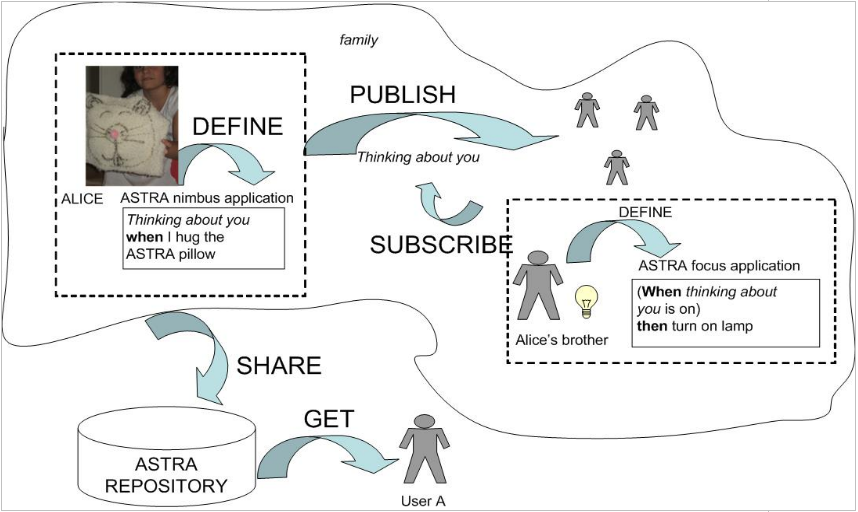
\includegraphics[scale=0.4]{screenshots/astra-applications-schema.png}
  \caption{\label{img:astra-applications-schema}ASTRA applications example}
 \end{center}
\end{figure}

\section{Motivations of the project}

The aim of this project is to create a system to manage the applications we
mentioned in Section \ref{subsec:intro-awareness-applications} and integrate
it into the ASTRA SOA (see Section \ref{subsubsec:tech-astra-soa}).
Managing comprises fuctionalities for sharing, tagging, locating,
appropriating and adapting the applications.
Figure \ref{img:astra-repository} shows the process of sharing and
appropriating applications through a central repository, illustrating the need
of customizing the parameters that are going to be shared (I.e.: for privacy
reasons) by user A, and the need of adapting the application to its
preferences (I.e.: connect it to his physical devices) by user B.
This process is potentially complex, therefore functionalities to help the user
to perform it are needed, as we will see in Section
\ref{subsec:implementation-app-adaptation}.
It is important to remark the difference between ``sharing'' and
``publishing''.  As we can see in Figure
\ref{img:astra-applications-schema}, sharing an application implies to upload a
taylorized set of information about it into the repository, but it does not
imply to send any kind of awareness information as in the case of publishing.
In the same way, ``retrieving"\footnote{We will use the verbs ``get'',
``appropriate'' or ``retrieve'' as synonyms when referring to an application in
this document.} an application from the repository implies to get it and taylorized
it, but not to subscribe to it.
On the other hand, once an user has appropriated and adapted the application, he
will be able to publish it as one made from the scratch.

\begin{figure}[h!]
 \begin{center}
 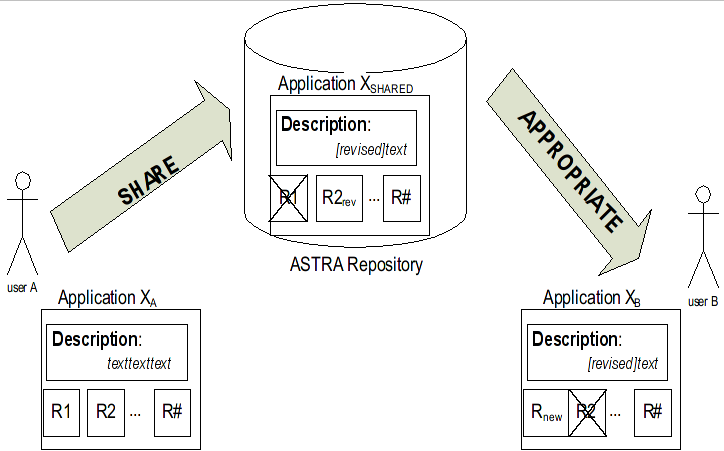
\includegraphics[scale=0.4]{screenshots/repository-appropiation.png}
  \caption{\label{img:astra-repository}Sharing and retrieving
  applications through the repository}
 \end{center}
\end{figure}

The rest of this document describes the process carried on to develop the
previously mentioned system, including a goals statement in Chapter
\ref{chap:objectives}, a explanation of the employed methodology and the
involved technologies in Chapter \ref{chap:methodology}, a detailed description
of the project in Chapter \ref{chap:description}, and a discussion of the
fulfillment of the goals and the personal contribution in Chapter
\ref{chap:conclusions}. 

%%Objectives
\chapter{Objectives}
\label{chap:objectives}

In this section we will state briefly the main goals of the project. The way in
which these objectives were achieved will be discussed in Chapter
\ref{chap:description}.
\par

The main objectives of this project are:

\begin{itemize}
  \item Create a main repository for applications, where the users can browse,
  share and retrieve them. This should be accomplished taking into account:
  \begin{itemize}
    \item The sharing process has to be flexible enough to allow the user
    choosing in which communities the application is going to be shared, and
    which rules are going to be shared.
    \item The retrieving process has to be flexible enough to allow the user a
    customization of the retrieved application. 
    \item The changes needed to adapt the application have to be as transparent
    to the user as possible.
    \item It is necessary to implement a mechanism which allows the user to
    search for applications:
      \begin{itemize}
        \item By different criteria: tags, description, type, etc.
        \item Using a system recommendation process, where the user just has to
        select an application and some similar applications will be suggested.
      \end{itemize}
  \end{itemize}
  
  \item Create a system which allows the users to tag the applications. This
  should be accomplished taking into account the need of different scopes for
  the tags:
  \begin{itemize}
    \item Private tags, which are only for personal purposes and should not be
    stored in the Backend.
    \item Community tags, which are only visible for members of that community.
    \item Public tags, which are visible for all the members.
  \end{itemize}
  
  
  \item Create a GUI which allows the user to carry out the operations defined
  previously. This should be performed taking into account:
  \begin{itemize}
    \item The GUI has to be connected with the rest of systems in a loose
    coupling way.
    \item It has to be intuitive.
    \item It has to be extensible, so other systems can be connected to it in
    the future.
  \end{itemize}
\end{itemize}


%%Methodology and technologies
\chapter{Methodology and involved technologies}
\label{chap:methodology}

\section{Methodology}
\label{section:methodology-spiral}

Due to the researching nature of the main project, it was quite difficult to
establish a fixed set of requirements in the beginning. Therefore, we used
the following system to carry on the process:

\begin{itemize}
  \item Establish a set of main objectives which can be expanded afterwards. The
  final result is the set of objectives which was discussed in Chapter
  \ref{chap:objectives}.
  \item Create a set of use cases based on these discussions.
  \item Create a design which has to be flexible enough to allow the
  introduction of new changes in the future.
  \item Implement a prototype and perform tests.
  \item Do a demonstration.
  \item New elicitation requirements process if necessary.
\end{itemize}

This model follows a spiral model (see Figure \ref{img:spiral}), a software
development process combining elements of both design and prototyping-in-stages, in an effort to combine 
advantages of top-down and bottom-up concepts.

\begin{figure}
 \begin{center}
 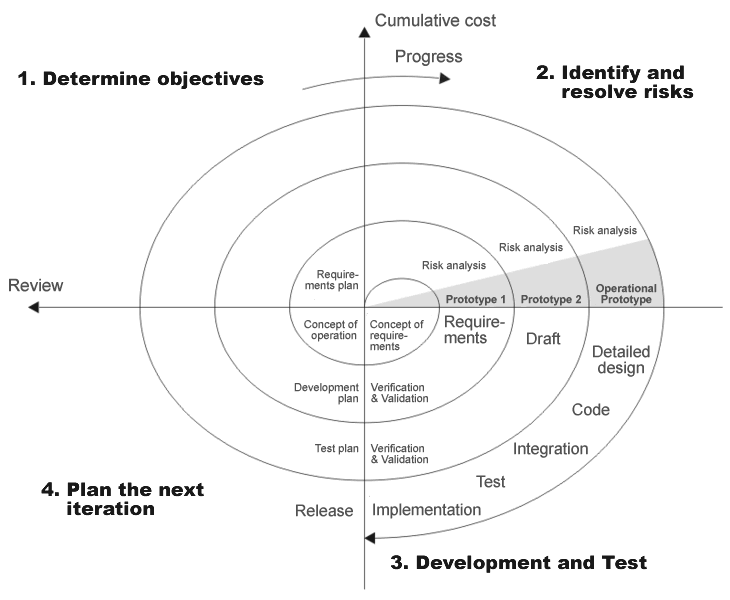
\includegraphics[scale=0.33]{img/spiral_model.png}
 \end{center}
 \caption{\label{img:spiral}Spiral model (Boehm, 1988)}
\end{figure}

Due to the limited extension of this document, it is not possible to explain in
the deserved detail the dynamic followed during the process. But it is
important to stand out at least that the whole process took four iterations
which are briefly explain in the Table \ref{table:iterations}.

%%\begin{center}
\begin{table}[h]
	\small
	\centering
	\begin{tabular}{||r|c|c||}
	\hline \hline
	Iteration & Requirements & Affected components
	\\
	\hline
	\hline 
	1 & Share and retrieve applications & \texttt{RepositoryManager} \& \texttt{PHP
	EUT tools}\\
	\hline
	2 & Tagging & \texttt{TagManagerNode} \& \texttt{TagManagerBackEnd} \\
	\hline
	3 & Searching capabilities & \texttt{RepositoryManager},\\
	  &	\& tagging extensions &\texttt{TagManagerNode} \& \texttt{TagManagerBackEnd}\\
	\hline
	4 & GUI & \texttt{ApplicationManager} \\
	\hline \hline
	\end{tabular}
	\caption{\label{table:iterations}Iterations during the project}
\end{table}
%%\end{center}

We have followed a methodology which can be seen as an Agile software
development methodology \cite{agile-paper}. The concept refers to a group of
software development methodologies based on iterative development, where requirements and  solutions
evolve through collaboration between self-organizing cross-functional teams. 
The term was coined in the year 2001 when the Agile Manifesto
\cite{agile-manifesto} was formulated.

Agile methods generally promote a disciplined project management  process that
encourages frequent inspection and adaptation, a leadership philosophy  that
encourages teamwork, self-organization and accountability, a set of 
engineering best practices that allow for rapid delivery of high-quality 
software, and a business approach that aligns development with customer needs
and company goals. Conceptual foundations of this framework are found in 
modern approaches to operations management and analysis, such as lean 
manufacturing, soft systems methodology, speech act theory (network of 
conversations approach), and Six Sigma.

This methodology fits properly with the researching
nature of the project and the fact that new requirements arise continuously.

%%The documentation which is discussed in the next sections refers to the
%%the final documentation produced as a consequence of all the iterations.

\section{Involved paradigms and technologies}

In this section we will explain briefly the main paradigms and technologies
involved during the achievement of this project.

%%SOA
\subsection{SOA}

Service Oriented Architecture is a paradigm for organizing and utilizing distributed capabilities 
that may be under the control of different ownership domains \cite{soa-principles}.
It provides a uniform means to offer, discover, interact with and use capabilities to produce 
desired effects consistent with measurable preconditions and expectations.
\par
In computing, the term Service-Oriented Architecture expresses a perspective
of software architecture that defines the use of services to support the requirements of software 
users. In an SOA environment, resources on a network are made available as independent services 
that can be accessed without knowledge of their underlying platform implementation.
SOA can also be regarded as a style of Information Systems architecture that
enables the creation of applications that are built by combining loosely coupled and 
inter-operable services.

The main principles behind the SOA paradigm can be summarized as follows:

\begin{itemize}
	\item Reuse
	\item Granularity
	\item Modularity
	\item Composability
	\item Componentization
	\item Interoperability
	\item Compliance to standards (both common and industry-specific) (e.g. Web
Services) 
	\item Services identification and categorization, provisioning and delivery,
and monitoring and tracking
\end{itemize}

\subsubsection{SOAP and Apache Axis}
\label{subsubsec:tech-soap-axis}
SOAP is a lightweight protocol for exchanging structured information in a 
decentralized, distributed environment \cite{w3c-soap-spec}. It is an XML (see
Section \ref{subsec:tech-xml}) based protocol that consists of three parts: an 
envelope that defines a framework for describing what is in a message and how 
to process it, a set of encoding rules for expressing instances of 
application-defined datatypes, and a convention for representing remote 
procedure calls and responses.

The implementation we have used is Apache Axis, it consists of an open source 
Java and C++ implementation of the SOAP server, and various utilities and APIs
for generating and deploying Web service applications. Using Apache Axis, 
it is possible to create interoperable and distributed computing applications.
Axis is developed under the auspices of the Apache Software Foundation.


\subsubsection{ASTRA SOA}
\label{subsubsec:tech-astra-soa}
The ASTRA Service-Oriented Architecture is the backbone of ASTRA 
\cite{astra-soa-white-paper}. It includes the platform for awareness services, 
the ontology, ontology management, context management, service discovery, and 
other necessary modules like the ones developed for this project.

These services are offered by a set of bundles (see Section \ref{subsec:tech-osgi})
that can be grouped into two subsystems from a high level point of view: ASTRA
Node and ASTRA Backend, following a Client-Server model\footnote{There has
been some discussion about the possibility of following a P2P model in ASTRA,
but this is out of the scope of the current implementation.}. Therefore it is
important to distinguish between the local and remote nature connection when 
consuming other bundles services, to take into account the limitations in the
type of objects we can use for our web services interfaces in the case of remote
connections, and to threat properly possible problems in the network.

Below are listed the bundles whose services have been used by the bundles
developed for this project. The dependencies with them are explained in Sections
\ref{subsubsec:connections-rm}, \ref{subsubsec:connections-tmbe},
\ref{subsubsec:connections-tmn} and \ref{subsubsec:connections-am}.

\begin{itemize}
  \item \verb|UserManager|: It is the responsible for managing users and their
  profiles, as well as the management of the user identities. It is executed in
  the Backend.
  \item \verb|CommunityManager|: It is the responsible for providing the
  possibility to define, share and connect virtual community representations in within which
  users can share awareness information. It is executed in the Backend.
  \item \verb|AwarenessManager|: It is the responsible for the connection
  between low level user-system interaction and the high level concepts related to
  them. It is connected with the Rules engine kernel. It is executed in the
  Nodes.
  \item \verb|AwarenessApplicationManager|: It is the responsible for storing
  and managing the local awareness applications. It is executed
  in the Nodes.
  \item \verb|OntologyManager|: It is the responsible for managing, looking-up
  and extending the ontologies. It is executed in the Nodes.
  \item \verb|PersistencyManager|: It is the responsible for providing storage
  functionalities. It is executed in the Backend and the Nodes.
  \item \verb|RemoteFrameworkManager|: It is the responsible for providing
  facilities to consume remote bundles services. It is executed in both subsystems.
  \item \verb|EventsManager|: It is the responsible for providing facilities to
  communicate events between the bundles. It is executed in both subsystems.
\end{itemize}



%Java
\subsection{Java}
Most of the development tasks during the project were coded using Java.
Java is a programming language originally developed by James Gosling at Sun 
Microsystems and released in 1995 as a core component of Sun Microsystems' Java
platform. The language derives much of its syntax from C and C++ but has a
simpler  object model and fewer low-level facilities. Java applications are 
typically compiled to bytecode (class file) that can run on any Java virtual 
machine (JVM) regardless of computer architecture.

The original and reference implementation Java compilers, virtual machines, 
and class libraries were developed by Sun from 1995. As of May 2007, in
compliance  with the specifications of the Java Community Process, Sun made 
available most of their Java technologies as free software under the GNU
General  Public License. Others have also developed alternative implementations
of these Sun technologies, such as the GNU Compiler for Java and GNU Classpath.

Java has significant advantages over other languages and environments  that
make it suitable for just about any programming task.

The advantages of Java are as follows:
\begin{itemize}
  \item Java is easy to learn: Java was designed to be easy to use and is
  therefore easier to write, compile, debug, and learn than other programming
  languages.
  \item Java is object-oriented: This allows us to create modular programs and
  reusable code.
  \item Java is platform-independent: One of the most significant
  advantages of Java is its ability to move easily from one computer system  to
  another. The ability to run the same program on many different systems is 
  crucial to World Wide Web software, and Java succeeds at this by being 
  platform-independent at both the source and binary levels.
\end{itemize}

Because of Java's robustness, ease of use, cross-platform  capabilities and
security features, it has become a language of choice for providing  worldwide
Internet solutions.


%%OSGi
\subsection{OSGi}
\label{subsec:tech-osgi}
%%\subsubsection{What is OSGi?}
OSGi (Open Services Gateway initiative) is a flexible framework, which provides
a standardized environment for service deployment and operation. 
The Framework implements an elegant, complete, and dynamic component
model; something that is missing in standalone Java/VM environments. The
platform is java-based and can be remotely managed.
In Figure \ref{img:osgi} we can see the OSGi layered model.

Applications or components (coming in the form of bundles for deployment) can
be remotely installed, started, stopped, updated and uninstalled without requiring a reboot. 
Bundles are deployed on an OSGi framework, the bundle runtime environment. 
This is not a container like Java Application Servers. It is a collaborative environment. 
Bundles run in the same VM and can actually share code. 
The framework uses the explicit imports and exports to wire up the bundles so they do not have 
to concern themselves with class loading.

\begin{figure}
 \begin{center}
 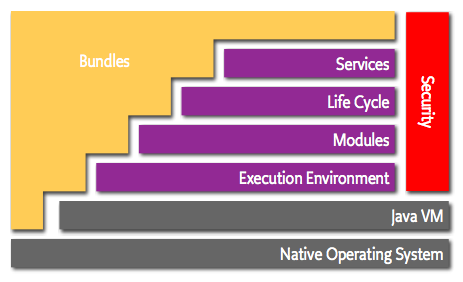
\includegraphics[scale=0.5]{img/layering-osgi.png}
 \end{center}
 \caption{\label{img:osgi}OSGi layered model}
\end{figure}

The original focus was on service gateways but the applicability turned out to be much wider. 
Implementations of the OSGi framework specification are available for a range of different 
environments and device classes, from backend systems via desktops to mobile devices. 
A well-known and popular usage for its flexibility is the Eclipse development framework, 
which is completely based on OSGi. The longest history can OSGi claim on embedded systems, 
where it originally was designed for. Currently Nokia is integrating OSGi technologies into 
their latest phones. 
But also big application servers like IBM WebSphere 6.1 start adapting this technology.

\subsubsection{OSGi-Knopflerfish}
\label{subsubsec:tech-osgi-knopflerfish}

Knopflerfish is a non-profit organization, developing OSGi related material. 
The project provides easy to use open source certified implementation of the OSGi R4 core 
framework specification, as well as related build tools and applications. 
Knopflerfish is available under a BSD style license.

\subsubsection{Why using OSGi in ASTRA?}
OSGi enforces a clean service oriented design approach, with a clear
distinction between interfaces and implementation. 
Services are deployed in bundles, which can be installed, updated and removed
during the runtime of the framework. OSGi is thus ideally suited to realizing
the principles of the SOA paradigm. OSGi also provides an Apache Axis (see
Section \ref{subsubsec:tech-soap-axis}) bundle that allows for automatic 
generation of web service interfaces.

The decision of using the OSGi framework has several severe impacts on the
design  of the functional components.
The most important implications for the component design are summarized here:
\begin{itemize}
	\item Services are de-coupled. A service must not take any assumptions about
the existence and life-cycle of any other service it might want to use (concept
of ``minimal assumptions'').
	\item Services communicate only through their exposed interfaces.
	\item A service must not take any assumptions about the implementation details
	of any other service. 
	The smallest unit for code deployment is a bundle, which might simply contain 
	API's or one or more service implementations.
\end{itemize}

It is worth stressing that OSGi is chosen as a platform, but it is
in no way a requirement by ASTRA to use OSGi. It is used because it offers a
flexible and convenient way of deploying the ASTRA SOA functional components. 
Any ASTRA component can be developed outside OSGi, and made available through a
Web Service interface.

%%Swing
\subsection{Swing}
Swing is a widget toolkit for Java. It is part of Sun Microsystems Java
Foundation Classes (JFC), an API for providing a graphical user interface (GUI)
for Java programs.

Swing was developed to provide a more sophisticated set of GUI components than
the earlier Abstract Window Toolkit. 
It provides a native look and feel that emulates the look and feel of several
platforms, and also supports a pluggable look and feel that allows applications
to have a look and feel unrelated to the underlying platform.

Swing has been used to develop a bundle which implements a GUI to allow the
user to perform all the operations related to the applications and tags
management process. The reason why Swing was chosen is the set of features that
its architecture provides:

\begin{itemize}
	\item Platform independence: Swing is platform independent both in terms of
its expression (Java) and its implementation (non-native universal rendering of
widgets).

	\item Extensibility: Swing is a highly partitioned architecture, which allows
  for the ``plugging'' of various custom implementations of specified framework
  interfaces: Users can provide their own custom implementation(s) of these 
  components to override the default implementations. In general, Swing users 
  can extend the framework by extending existing (framework) classes and/or 
  providing alternative implementations of core components.

	\item Component-oriented:  Swing is a component-based framework. The
	distinction between objects and components is a fairly subtle point: 
	concisely, a component is a well-behaved object with a known/specified 
	characteristic pattern of behaviour. Swing objects asynchronously fire 
	events, have ``bound'' properties, and respond to a well-known set of 
	commands (specific to the component). Specifically, Swing components are  Java
	Beans components, compliant with the Java Beans Component Architecture 
	specifications.

	\item Customizable: Given the programmatic rendering model of the Swing
	framework, fine control over the details of rendering of a component is 
	possible in Swing. As a general pattern, the visual representation of a Swing 
	component is a composition of a standard set of elements, such as a
	``border'', ``inset'', decorations, etc. Typically, users will
	programmatically customize a standard Swing component (such as a
	\verb|JTable|) by assigning specific Borders, Colors, Backgrounds, opacities,
	etc., as the properties of that component. The core component  will then use
	these property (settings) to determine the appropriate renderers to use in
	painting its various aspects. However, it is also completely possible to
	create unique GUI controls with highly customized visual representation.

	\item Configurable: Swing's heavy reliance on runtime mechanisms and indirect 
	composition patterns allows it to respond at runtime to fundamental changes 
	in its settings. For example, a Swing-based application can change its look 
	and feel at runtime. Further, users can provide their own look and feel 
	implementation, which allows for uniform changes in the look and feel of 
	existing Swing applications without any programmatic change to the application
	code.
\end{itemize}

These traits allowed us to fulfill successfully the requirements for the
above-mentioned bundle, which will be explained deeply in Sections
\ref{subsec:am-design} and \ref{subsec:implementation-mvc-swing}.

%XML
\subsection{XML}
\label{subsec:tech-xml}
XML (eXtensible Markup Language) is a general-purpose specification for
creating  custom markup languages. It is classified as an extensible
language,  because it allows the user to define the mark-up elements.

XML's purpose is to aid information systems in sharing structured data, 
especially via the Internet, to encode documents, and to serialize data;  in
the last context, it compares with text-based serialization languages such as 
JSON, YAML, and S-Expressions.

XML's set of tools helps developers in creating web pages but its usefulness
goes well beyond that. XML, in combination with other standards, makes  it
possible to define the content of a document separately from its formatting, 
making it easy to reuse that content in other applications or for other 
presentation environments. Most importantly, XML provides a basic syntax  that
can be used to share information between different kinds of computers, 
applications and organizations without needing to  pass
through many layers of conversion.

XML began as a simplified subset of the Standard Generalized Markup Language 
(SGML), meant to be readable by people via semantic constraints.
Application languages can be implemented in XML. These include XHTML, RSS,
MathML, GraphML, Scalable Vector Graphics, MusicXML, and others. Moreover, XML
is sometimes used as the specification language for such application languages.

XML is recommended by the World Wide Web Consortium (W3C). It is a fee-free 
open standard. The recommendation specifies lexical grammar and parsing 
requirements.

As we will explain in detail in Section
\ref{subsec:implementation-app-adaptation}, XML is the language used to
represent the rules in ASTRA.

%DOM
\subsection{DOM}
\label{subsec:tech-dom}
The Document Object Model (DOM) is a cross-platform and language-independent 
convention for representing and interacting with objects in HTML, XHTML and 
XML documents. Objects under the DOM (also sometimes called ``Elements'') may be
specified and addressed according to the syntax and rules of the programming 
language used to manipulate them. The rules for programming and interacting
with the DOM are specified in the DOM Application Programming Interface (API).


As we will explain in detail in Section
\ref{subsec:implementation-app-adaptation}, DOM was used to access and modify
the rules in ASTRA.


%%Lucene
\subsection{Lucene}
\label{sec:tech-lucene}
Apache Lucene is an open source information retrieval library, originally
created in Java by Doug Cutting. 
It is supported by the Apache Software Foundation and is released under the Apache 
Software License.
Lucene itself is just an indexing and search library and does not contain 
crawling and HTML parsing functionality: it is not an application. 
It allowed us to create a search engine integrated in one of the bundles
(see Sections \ref{subsec:repository-design} and
\ref{subsec:implementation-search-engine}) to offer searching capabilities in
it. The main reasons why Lucene was proposed (and accepted) were:

\begin{itemize}
	\item It is open-source.
	\item It has a great performance.
	\item It is quite flexible and easy to extend if more functionalities are 
	needed in the future.
	\item It is cross-platform.
\end{itemize}


%MySQL
\subsection{MySQL}
\label{subsec:tech-mysql}
MySQL is a relational database management system (RDBMS) very popular in the
free and open source software communities. The program runs as a server
providing multi-user access to a number of databases.

The project's source code is available under terms of the GNU General Public 
License, as well as under a variety of proprietary agreements. MySQL is owned 
and sponsored by a single for-profit firm, the Swedish company MySQL AB, now  a
subsidiary of Sun Microsystems, which holds the copyright of most of the code.

MySQL is commonly used by free software projects which require a full-featured
database management system, such as WordPress, phpBB and other software built 
on the LAMP software stack. It is also used in very high-scale World Wide Web 
products including Google and Facebook.

MySQL is the RDBMS system which is used for taking care of the persistence
in ASTRA.


%%Description
\chapter{Description}
\label{chap:description}

In this chapter we will detail the process carried on to transform the
initial objectives into requirements, and the design and development of the
application based on them.

%%intro
%%%%%%%%%%%%%%% Requirements %%%%%%%%%%%%%%%%%%%%%%%%%
\section{Requirements}
\label{sec:requirements}

In this section we will describe shortly the requirements that we gathered
during the several requirements elicitation processes performed during all the
iterations (see Table \ref{table:iterations}). 
It is interesting to remark that this process becomes even more important (and
challenging) in projects of a researching nature like ASTRA, due to the
continuous rise of requirements implicit in its kind.

Tables \ref{table:functional-requirements} and
\ref{table:non-functional-requirements} summarize the most important functional
and non functional requirements that we gathered respectively.
%%Functional requirements
\begin{table}[h!]
	\small
    \begin{center}
		\begin{tabular}{||r|l||}
		\hline \hline
		\multicolumn{2}{||c||}{\bfseries{Functional requirements}} \\
		\hline \hline
			1. & Create a repository to store awareness applications. \\
			\hline
			2. & The information to share can be customized by the user before being
			stored.\\
			\hline
			3. & The repository has to take into account the visibility of the
			applications\\
			   & in terms of communities.\\
			\hline
			4. & It is necessary to offer functionalities to browse the repository
			by communities.\\
			\hline
		 	5. & It is necessary to create a mechanism to search applications by
		 	different \\
		 	  & criteria (tags, description, type or any).	\\
			\hline
		 	6. & It is necessary to create a mechanism to recommend applications 
		 	based \\
		 	 & on the similarity with respect to another application.\\
			\hline
		 	7. & During the appropriation of an application, it is necessary to
		 	offer \\
		 	& the user the possibility of customizing the application (i.e.:
		 	choosing the rules).\\
		 	\hline
		 	8. & Create a mechanism to obtain a ``human readable'' description of a
		 	rule.\\
		 	\hline
		 	9. & Create a system which allows us to tag applications choosing the
		 	visibility:\\
		 	& public, communities or private.\\
			\hline
		 	10. & Create a GUI which allows the interaction with the repository 
		 	and perform \\
		 	& common operations (logging in, showing help, etc.).\\
		 	
		
		\hline \hline
		\end{tabular}
		\caption{\label{table:functional-requirements}Functional requirements}
	\end{center}
\end{table}


%%Non-Functional requirements
\begin{table}[h!]
	\small
    \begin{center}
		\begin{tabular}{||r|l||}
		\hline \hline
		\multicolumn{2}{||c||}{\bfseries{Non functional requirements}} \\
		\hline \hline
			1. & The functionalities have to be offered by OSGi bundles through
			their  \\
			& web services interfaces. \\
			\hline
			2. & The system has to perform the retrieving process as transparent
			 as possible \\
			& for the user. \\
			\hline
			3. & All the components have to be multiplatform. \\
			\hline
			4. & The GUI has to be intuitive.\\
			\hline
			5. & The GUI has to be easy to connect to other bundles in the future.\\
			\hline
		 	6. & It is necessary to study the possibility of using ontology services
		 	provided\\
		 	& by \verb|OntologyManager| in order to improve the performance of some\\
		 	& of the functionalities (i.e.: application adaptation).\\
		
		\hline \hline
		\end{tabular}
		\caption{\label{table:non-functional-requirements}Non functional requirements}
	\end{center}
\end{table}
\clearpage

%%use cases
%%%%%%%%%%%%%%% Use cases %%%%%%%%%%%%%%%%%%%%%%%%%

\section{Use cases}
\label{sec:use-cases}

In this section we will state the main use cases identified and we detail the
interactions of the main scenarios for each of them.

%%%%%%%%%%%%%%% Repository Management %%%%%%%%%%%%%%%%%%%%%%%%%

\subsection{Repository management}
\label{subsec:rm-use-cases}
The Figure \ref{img:uc-repository} shows the main use cases related with the
repository management process, which are detailed in Tables
\ref{table:browse-app}, \ref{table:share-app} and \ref{table:retrieve-app}.

\begin{figure}[h!]
 \begin{center}
 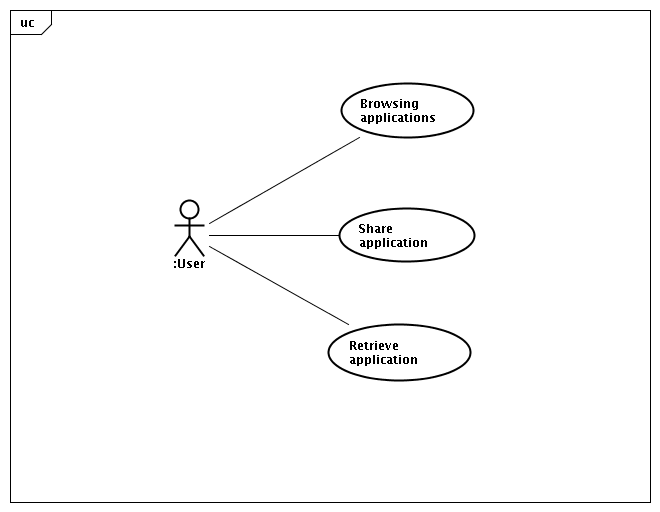
\includegraphics[scale=0.5]{diagrams/UseCasesDiagram-sharing.png}
  \caption{\label{img:uc-repository}Repository management use cases}
 \end{center}
\end{figure}


%%Browse applications
\begin{table}[h!]
	\small
    \begin{center}
		\begin{tabular}{||r|l||}
		\hline \hline
		\multicolumn{2}{||c||}{\bfseries{Browse applications}} \\
		\hline
		\hline 
		Brief description: & Actor browses repository applications. \\
		\hline
		Actors: & Authenticated ASTRA user. \\
		\hline
		Preconditions: &  There are applications visible for that user. \\
		\hline \hline
		\multicolumn{2}{||l||}{Basic flow of events:} \\
		\hline \hline
			1. & User expands the applications tree. \\
			2. & User selects an application. \\
			3. & System retrieves all the information related to it.	\\ 
			4. & System displays the information. \\ \hline \hline
		Postconditions: &  - \\
		\hline \hline
		\end{tabular}
		\caption{\label{table:browse-app} Browse applications - general scenario
		description}
	\end{center}
\end{table}

%%Share application
\begin{table}[h!]
	\small
    \begin{center}
		\begin{tabular}{||r|l||}
		\hline \hline
		\multicolumn{2}{||c||}{\bfseries{Share application}} \\
		\hline
		\hline 
		Brief description: & Actor shares an application in the repository. \\
		\hline
		Actors: & Authenticated ASTRA user. \\
		\hline
		Preconditions: &  A local application has been selected. \\
		\hline \hline
		\multicolumn{2}{||l||}{Basic flow of events:} \\
		\hline \hline
			1. & User selects share application. \\
			2. & System displays all the information related to it. \\
			3. & User customizes the parameters to be shared: \\ 
			   & visibility in terms of communities, rules, description, etc.	\\ 
			4. & User confirms the sharing process. \\ 
			5. & System validates the parameters. \\
			6. & System confirms the application was shared properly. \\\hline \hline
		Postconditions: &  A new application is available in the repository. \\
		\hline \hline
		\end{tabular}
		\caption{\label{table:share-app} Share application - general scenario
		description}
	\end{center}
\end{table}

%%Retrieve application
\begin{table}[h!]
	\small
    \begin{center}
		\begin{tabular}{||r|l||}
		\hline \hline
		\multicolumn{2}{||c||}{\bfseries{Retrieve application}} \\
		\hline
		\hline 
		Brief description: & Actor retrieves an application from the repository. \\
		\hline
		Actors: & Authenticated ASTRA user. \\
		\hline
		Preconditions: &  An application from the repository has been selected. \\
		\hline \hline
		\multicolumn{2}{||l||}{Basic flow of events:} \\
		\hline \hline
			1. & User selects retrieve application. \\
			2. & System displays all the information related to it. \\
			3. & User customizes the parameters to be retrieved: rules and description.	\\ 
			4. & User confirms the retrieving process. \\ 
			5. & System validates the parameters. \\
			6. & System confirms the application was retrieved properly. \\\hline \hline
		Postconditions: &  A new application is available in the user local space. \\
		\hline \hline
		\end{tabular}
		\caption{\label{table:retrieve-app} Retrieve application - general scenario
		description}
	\end{center}
\end{table}


%%%%%%%%%%%%%%% Searching %%%%%%%%%%%%%%%%%%%%%%%%%
\clearpage

\subsection{Searching}
\label{subsec:searching-use-cases}
The Figure \ref{img:uc-searching} shows the main use cases related with the
searching requirements, which are detailed in Tables
\ref{table:search-criteria} and \ref{table:search-similarity}.

\begin{figure}[h!]
 \begin{center}
 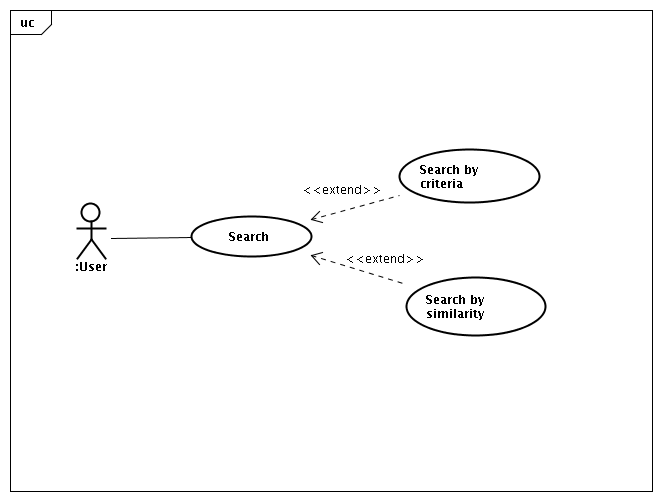
\includegraphics[scale=0.5]{diagrams/UseCasesDiagram-searching.png}
 \end{center}
 \caption{\label{img:uc-searching}Searching use cases}
\end{figure}

%%Search by criteria
\begin{table}[h!]
	\small
    \begin{center}
		\begin{tabular}{||r|l||}
		\hline \hline
		\multicolumn{2}{||c||}{\bfseries{Searching by criteria}} \\
		\hline
		\hline 
		Brief description: & Actor searches for an application typing some keywords
		and a criterion.\\
		\hline
		Actors: & Authenticated ASTRA user. \\
		\hline
		Preconditions: &  - \\
		\hline \hline
		\multicolumn{2}{||l||}{Basic flow of events:} \\
		\hline \hline
			1. & User enters one or more keywords. \\
			2. & User selects a criterion (by tags, by description, by type or any). \\
			3. & System performs a search based on the given parameters. \\
			4. & System displays matching applications.\\ 
		\hline \hline
		Postconditions: &  - \\
		\hline \hline
		\end{tabular}
		\caption{\label{table:search-criteria}Search by criteria - general scenario
		description}
	\end{center}
\end{table}

%%Search by similarity
\begin{table}[h!]
	\small
    \begin{center}
		\begin{tabular}{||r|l||}
		\hline \hline
		\multicolumn{2}{||c||}{\bfseries{Searching by similarity}} \\
		\hline
		\hline 
		Brief description: & Actor searches for applications that are similar to a
		given application.\\
		\hline
		Actors: & Authenticated ASTRA user. \\
		\hline
		Preconditions: &  - \\
		\hline \hline
		\multicolumn{2}{||l||}{Basic flow of events:} \\
		\hline \hline
			1. & User selects an application. \\
			2. & System compares the selected application with \\ 
			  & applications in the repository using different measures. \\ 
			3. & System displays matching applications.\\ 
		\hline \hline
		Postconditions: &  - \\
		\hline \hline
		\end{tabular}
		\caption{\label{table:search-similarity}Search by similarity - general
		scenario description}
	\end{center}
\end{table}



%%%%%%%%%%%%%%% Tags management %%%%%%%%%%%%%%%%%%%%%%%%%
\clearpage

\subsection{Tags management}
\label{subsec:tags-use-cases}

The Figure \ref{img:uc-tagging} shows the main use cases related with the
tags management process, which are detailed in Tables \ref{table:add-tag}
and \ref{table:remove-tag}.

\begin{figure}[h!]
 \begin{center}
 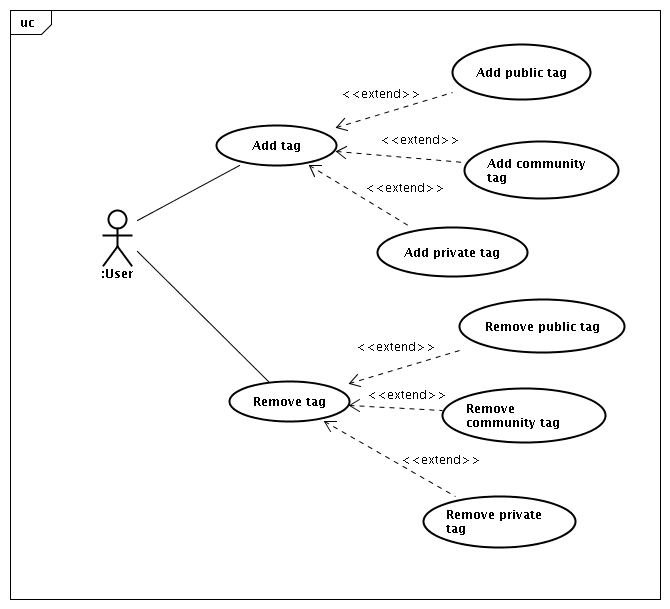
\includegraphics[scale=0.5]{diagrams/UseCasesDiagram-tagging.png}
 \end{center}
 \caption{\label{img:uc-tagging}Tagging use cases}
\end{figure}


%%Add tag
\begin{table}[h!]
	\small
    \begin{center}
		\begin{tabular}{||r|l||}
		\hline \hline
		\multicolumn{2}{||c||}{\bfseries{Add tag}} \\
		\hline
		\hline 
		Brief description: & Actor adds a tag to an application specifying the level\\
		& of visibility of the tag. \\
		\hline
		Actors: & Authenticated ASTRA user. \\
		\hline
		Preconditions: & An application has been selected. \\
		\hline \hline
		\multicolumn{2}{||l||}{Basic flow of events:} \\
		\hline \hline
			1. & User enters a tag name. \\
			2. & User specifies tag visibility. \\
			3. & System validates tag. \\
			4. & System stores the tag. \\ 
			5. & System confirms that tag has been added. \\
		\hline \hline
		Postconditions: & A new tag is associated to the application \\
		&  and is made available within the proper scope. \\
		\hline \hline
		\end{tabular}
		\caption{\label{table:add-tag} Add tag - general scenario description}
	\end{center}
\end{table}

%%Remove tag
\begin{table}[h!]
	\small
    \begin{center}
		\begin{tabular}{||r|l||}
		\hline \hline
		\multicolumn{2}{||c||}{\bfseries{Remove tag}} \\
		\hline
		\hline 
		Brief description: & Actor removes a tag from an application. \\
		\hline
		Actors: & Authenticated ASTRA user. \\
		\hline
		Preconditions: & User has previously tagged the selected application. \\
		\hline \hline
		\multicolumn{2}{||l||}{Basic flow of events:} \\
		\hline \hline
			1. & User selects a tag. \\
			2. & System displays option to remove the tag. \\
			3. & User chooses to remove the tag. \\
			4. & System deletes the tag.\\ 
			5. & System confirms that tag has been deleted. \\
		\hline \hline
		Postconditions: & The specified tag is no longer associated with the
		specified application. \\ \hline \hline
		\end{tabular}
		\caption{\label{table:remove-tag}Remove tag - general scenario description}
	\end{center}
\end{table}

%%%%%%%%%%%%%%% Others %%%%%%%%%%%%%%%%%%%%%%%%%
\clearpage

\subsection{Other general functionalities}
\label{subsec:others-use-cases}
The Figure \ref{img:uc-others} shows use cases that capture other general
functionalities, which are detailed in Tables \ref{table:login}, 
\ref{table:logout} and \ref{table:help}.

\begin{figure}[h!]
 \begin{center}
 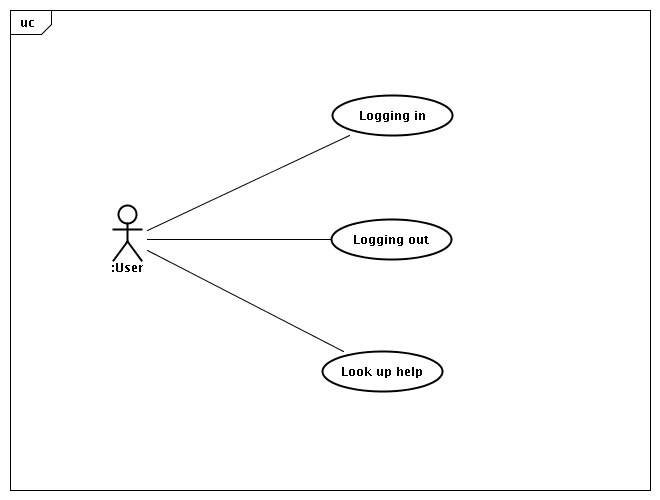
\includegraphics[scale=0.5]{diagrams/UseCasesOthers.png}
 \end{center}
 \caption{\label{img:uc-others}Other general functionalities}
\end{figure}

%%Logging in
\begin{table}[h!]
	\small
    \begin{center}
		\begin{tabular}{||r|l||}
		\hline \hline
		\multicolumn{2}{||c||}{\bfseries{Logging in}} \\
		\hline
		\hline 
		Brief description: & Actor logs in the system.\\
		\hline
		Actors: & Non-authenticated ASTRA user. \\
		\hline
		Preconditions: &  Login window is displayed. \\
		\hline \hline
		\multicolumn{2}{||l||}{Basic flow of events:} \\
		\hline \hline
			1. & User types username and password. \\
			2. & System validates them. \\
			3. & System loads user's profile. \\ 
			4. & System displays the main menu and disposes the login window. \\
			\hline \hline Postconditions: &  - \\
		\hline \hline
		\end{tabular}
		\caption{\label{table:login}Logging in - general scenario  description}
	\end{center}
\end{table}

%%Logging out
\begin{table}[h!]
	\small
    \begin{center}
		\begin{tabular}{||r|l||}
		\hline \hline
		\multicolumn{2}{||c||}{\bfseries{Logging out}} \\
		\hline
		\hline 
		Brief description: & Actor logs out of the system. \\
		\hline
		Actors: & Authenticated ASTRA user. \\
		\hline
		Preconditions: &  Main window is displayed. \\
		\hline \hline
		\multicolumn{2}{||l||}{Basic flow of events:} \\
		\hline \hline
			1. & User selects logout option. \\
			2. & System asks for confirmation. \\
			3. & User confirms. \\ 
			4. & System closes user's session, disposes the main window and \\
			   & displays the login window \\ 
		\hline \hline Postconditions: &  - \\
		\hline \hline
		\end{tabular}
		\caption{\label{table:logout}Logging out - general scenario description}
	\end{center}
\end{table}

%%Lookup help
\begin{table}[h!]
	\small
    \begin{center}
		\begin{tabular}{||r|l||}
		\hline \hline
		\multicolumn{2}{||c||}{\bfseries{Look up help}} \\
		\hline
		\hline 
		Brief description: & Actor looks up the online help. \\
		\hline
		Actors: & Authenticated ASTRA user. \\
		\hline
		Preconditions: &  -  \\
		\hline \hline
		\multicolumn{2}{||l||}{Basic flow of events:} \\
		\hline \hline
			1. & User selects online help option. \\
			2. & System retrieves the remote help. \\
			3. & System displays the help contents in an intuitive way. \\ 
			\hline \hline
		Postconditions: &  - \\
		\hline \hline
		\end{tabular}
		\caption{\label{table:help}Look up help - general scenario description}
	\end{center}
\end{table}
\clearpage

%%design
%%%%%%%%%%%%%%%%%%%%%%%%% Design %%%%%%%%%%%%%%%%%%%%%%%

\section{Design}

In this section we will explain the most important design decisions and the
reasons why they were taken. We will also go into detail in the most
remarkable characteristics.


%% Intro
\subsection{Bundles design}
\label{subsec:bundles-design}
One of the first and most important decisions is how to divide the
functionality into components. Having the requirement of using OSGi, it seems
natural to use a bundle as the notion of component.
The final design consists of four bundles:

\begin{itemize}
	\item \verb|RepositoryManager|, which has the following responsibilities:
	  	\begin{itemize}
	        \item Offer services to share applications.
	        \item Offer services to retrieve applications.
	        \item Storage of shared applications.
	        \item Offer services to search applications by criteria.
	        \item Offer services to search applications by similarity.
          \end{itemize} 
          
	\item \verb|TagManagerBackEnd|, which has the following responsibilities:
	  	\begin{itemize}
	        \item Offer services to add and delete public and community tags.
	        \item Offer services to retrieve those tags in different and flexible
	        ways.
          \end{itemize} 
          
	\item \verb|TagManagerNode|, which has the following responsibilities:
	  	\begin{itemize}
	        \item Offer services to add and delete private tags.
	        \item Offer services to retrieve those tags in different and flexible
	        ways.
        \end{itemize} 
          
	\item \verb|ApplicationManager|, which is responsible of the interaction with
	the user, and connects with the proper bundles to satisfy his requests.
      
\end{itemize}

The components diagram in Figure \ref{img:bundles-components-main} shows the
connection between all of them through its interfaces\footnote{The connection
with the rest of ASTRA bundles is omitted for simplicity reasons, but it will 
be discussed in the section where every bundle is explained.}:

\begin{figure}[h!]
 \begin{center}
 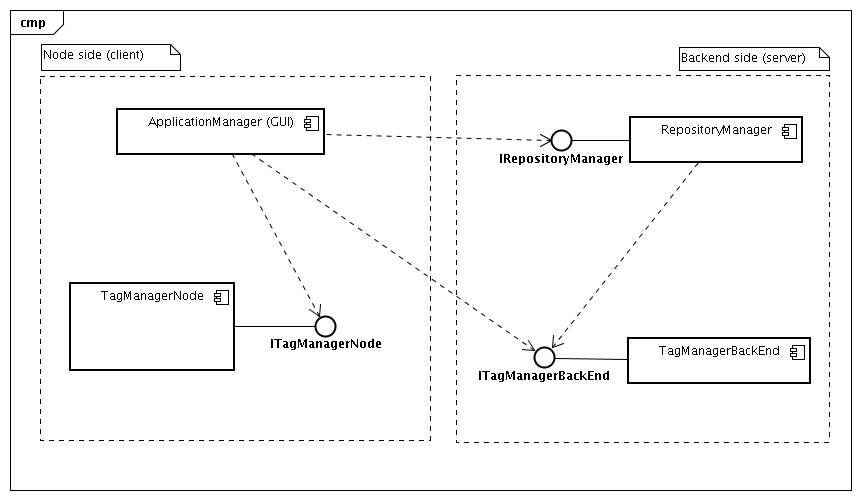
\includegraphics[scale=0.4]{diagrams/BundlesComponentsDiagram.png}
  \caption{\label{img:bundles-components-main}Relationships between the bundles
  developed for this project (components diagram)}
 \end{center}
\end{figure}

Sections \ref{subsec:repository-design}, \ref{subsec:tmbe-design},
\ref{subsec:tmn-design} and \ref{subsec:am-design} explain the most important
features of each of them.

%%%%%%%%%%%%%%% RepositoryManager %%%%%%%%%%%%%%%%%%%%%%%%%

\subsection{RepositoryManager}
\label{subsec:repository-design}

Since one of the most important goals of the project is the need of allowing
the users to share and retrieve applications, \verb|RepositoryManager| is one of
the key pieces of the project.
This bundle is executed in the Backend (server-side), and it offers a clear
interface to make its services available for the rest of the bundles
in ASTRA.

In this section we will explain the process we followed to perform its design.
Some of the trickiest implementation details about this bundle are explained
in Section \ref{sec:implementation}.

\subsubsection{Connection with other bundles}
\label{subsubsec:connections-rm}
The first step consists of analyzing the relationship between this bundle and
the rest of bundles in ASTRA.
Taking into account the requirements stated in Section \ref{sec:requirements}
and the analysis performed in Sections \ref{subsec:rm-use-cases} and
\ref{subsec:searching-use-cases}, we needed to make use of the services of  the
following bundles:

\begin{itemize}
  \item \verb|CommunityManager|: Necessary to retrieve information about the
  relationship between users, their communities and the applications. I.e.: to
  assure the visibility of certain application taking into account the
  communities joined for an user who is going to retrieve applications.
  \item \verb|TagManagerBackEnd|\footnote{The design of this bundle is explained
  in Section \ref{subsec:tmbe-design}}: Necessary to analyze the tags in order to
  construct the index of the search engine.
  \item \verb|EventsManager|: Necessary to keep track of the events produced
  in\\ \verb|TagManagerBackEnd|, in order to keep the index of the search engine updated.
  I.e: new tags or tags that have been deleted.
  \item \verb|PersistencyManager|: Necessary to store permanently all the data
  into the database. Using its services, we assure the robustness of the system.
\end{itemize}

The Figure \ref{img:rm-components} shows graphically the relationship between
\verb|RepositoryManager| and the rest of components through its interfaces.

\begin{figure}[h!]
 \begin{center}
 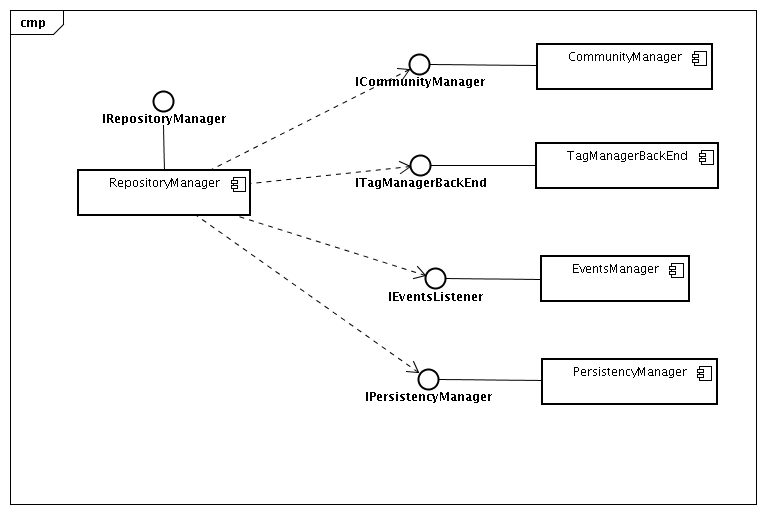
\includegraphics[scale=0.4]{diagrams/RepositoryManagerComponentsDiagram.png}
  \caption{\label{img:rm-components}RepositoryManager (components diagram)}
 \end{center}
\end{figure}

\subsubsection{Interface definition}

The next step carried on was defining an interface. The Tables
\ref{table:rm-interface-1}, \ref{table:rm-interface-2},
\ref{table:rm-interface-3} and \ref{table:rm-interface-4} summarize the
methods offered by the final version of \verb|RepositoryManager|.

%%tables with repository inteface
%%% Tables for repository interface %%%%
\begin{table}[h!]
	\small
    \begin{center}
		\begin{tabular}{||r|l|l||}
        
        %%%%%%%% Begin method %%%%%%%%%%%%%%%%%%
		\hline \hline
		\multicolumn{3}{||c||}{\bfseries{createSharedApplication}} \\
		\hline
		\hline 
		\multicolumn{3}{||l||}{Description: Create a new shared application in the
		repository.} \\
		\hline \hline
			Parameter & Type & Description \\
		\hline \hline
			appId & String & Application identifier in the standard ASTRA format. \\
			userId & String & Identifier of the user who uploads the application. \\
			appType & String & Type of application. \\
			appDescription & String & Application description. \\
		\hline \hline
		\multicolumn{3}{||l||}{Returns: Boolean, true if everything is ok, false if
		there was a failure.} \\
		\hline \hline
		%%%%%%%%%%%% End method %%%%%%%%%%%%%%%%%%%%%%
		
		%%%%%%%% Begin method %%%%%%%%%%%%%%%%%%
		\hline \hline
		\multicolumn{3}{||c||}{\bfseries{deleteSharedApplication}} \\
		\hline
		\hline 
		\multicolumn{3}{||l||}{Description: Delete a SharedApplication in the
		repository.} \\ \hline \hline
			Parameter & Type & Description \\
		\hline \hline
			appId & String & Application identifier in the standard ASTRA format \\
		\hline \hline
		\multicolumn{3}{||l||}{Returns: Boolean, true if the application was deleted
		properly, false otherwise.} \\
		\hline \hline
		%%%%%%%%%%%% End method %%%%%%%%%%%%%%%%%%%%%%
		
		%%%%%%%% Begin method %%%%%%%%%%%%%%%%%%
		\hline \hline
		\multicolumn{3}{||c||}{\bfseries{shareInCommunity}} \\
		\hline
		\hline 
		\multicolumn{3}{||l||}{Description: Store relationship between a shared 
		application and a community.} \\ \hline \hline
			Parameter & Type & Description \\
		\hline \hline
			userId & String & User identifier in the standard format. \\
			appId & String & Application identifier in the standard ASTRA format. \\
			communityId & String & Community identifier in the standard format. \\
		\hline \hline
		\multicolumn{3}{||l||}{Returns: Boolean, true if the operation was successful,
		false otherwise.} \\ \hline \hline
		%%%%%%%%%%%% End method %%%%%%%%%%%%%%%%%%%%%%
		
		%%%%%%%% Begin method %%%%%%%%%%%%%%%%%%
		\hline \hline
		\multicolumn{3}{||c||}{\bfseries{createSharedRule}} \\
		\hline
		\hline 
		\multicolumn{3}{||l||}{Description: Create a new shared rule associated to
		the application.} \\ \hline \hline Parameter & Type & Description \\
		\hline \hline
			userId & String & User identifier in the standard format. \\
			appId & String & Application identifier in the standard ASTRA format. \\
			ruleId & String & Rule identifier in the standard format. \\
			xmlData & String & XML file which contains the rule. \\
		\hline \hline
		\multicolumn{3}{||l||}{Returns: Boolean, true if the operation was successful,
		false otherwise.} \\ \hline \hline
		%%%%%%%%%%%% End method %%%%%%%%%%%%%%%%%%%%%%
		
		\end{tabular}
		\caption{\label{table:rm-interface-1} RepositoryManager interface}
	\end{center}
\end{table}


\begin{table}[h!]
	\small
    \begin{center}
		\begin{tabular}{||r|l|l||}

        %%%%%%%% Begin method %%%%%%%%%%%%%%%%%%
		\hline \hline
		\multicolumn{3}{||c||}{\bfseries{listSharedApplications}} \\
		\hline
		\hline 
		\multicolumn{3}{||l||}{Description: Returns the list of applications in the
		repository visible for that user.} \\ 
		\hline \hline 
		Parameter & Type & Description \\ 
		\hline \hline
			userId & String & User identifier in the standard format. \\
		\hline \hline
		\multicolumn{3}{||l||}{Returns: String array, list of applications.} \\
		\hline \hline
		%%%%%%%%%%%% End method %%%%%%%%%%%%%%%%%%%%%%
        
		%%%%%%%% Begin method %%%%%%%%%%%%%%%%%%
		\hline \hline
		\multicolumn{3}{||c||}{\bfseries{listSharedRules}} \\
		\hline
		\hline 
		\multicolumn{3}{||l||}{Description: Returns the list of rules in the
		repository associated to appID} \\ 
		\hline \hline 
		Parameter & Type & Description \\ 
		\hline \hline
			appId & String & Application identifier in the standard ASTRA format. \\
		\hline \hline
		\multicolumn{3}{||l||}{Returns: String array, list of rule identifiers.} \\
		\hline \hline
		%%%%%%%%%%%% End method %%%%%%%%%%%%%%%%%%%%%%
		
		%%%%%%%% Begin method %%%%%%%%%%%%%%%%%%
		\hline \hline
		\multicolumn{3}{||c||}{\bfseries{getXmlData}} \\
		\hline
		\hline 
		\multicolumn{3}{||l||}{Description: Returns the XML file which describes the
		rule.} \\ \hline \hline 
		Parameter & Type & Description \\ 
		\hline \hline
			appId & String & Application identifier in the standard ASTRA format. \\
			ruleId & String & Rule identifier in the standard format. \\
		\hline \hline
		\multicolumn{3}{||l||}{Returns: String, XML file describing the rule.} \\
		\hline \hline
		%%%%%%%%%%%% End method %%%%%%%%%%%%%%%%%%%%%%
		
		%%%%%%%% Begin method %%%%%%%%%%%%%%%%%%
		\hline \hline
		\multicolumn{3}{||c||}{\bfseries{getSharedApplicationName}} \\
		\hline
		\hline 
		\multicolumn{3}{||l||}{Description: Returns the name of the application.} \\
		\hline \hline Parameter & Type & Description \\ 
		\hline \hline
			appId & String & Application identifier in the standard ASTRA format. \\
		\hline \hline
		\multicolumn{3}{||l||}{Returns: String, application name.} \\
		\hline \hline
		%%%%%%%%%%%% End method %%%%%%%%%%%%%%%%%%%%%%
	
		%%%%%%%% Begin method %%%%%%%%%%%%%%%%%%
		\hline \hline
		\multicolumn{3}{||c||}{\bfseries{getSharedApplicationOwner}} \\
		\hline
		\hline 
		\multicolumn{3}{||l||}{Description: Returns the owner of the application.} \\
		\hline \hline Parameter & Type & Description \\ 
		\hline \hline
			appId & String & Application identifier in the standard ASTRA format. \\
		\hline \hline
		\multicolumn{3}{||l||}{Returns: String, application owner.} \\
		\hline \hline
		%%%%%%%%%%%% End method %%%%%%%%%%%%%%%%%%%%%%		
		
		%%%%%%%% Begin method %%%%%%%%%%%%%%%%%%
		\hline \hline
		\multicolumn{3}{||c||}{\bfseries{getSharedApplicationDescription}} \\
		\hline
		\hline 
		\multicolumn{3}{||l||}{Description: Returns the description of the
		application.} \\ \hline \hline Parameter & Type & Description \\ 
		\hline \hline
			appId & String & Application identifier in the standard ASTRA format. \\
		\hline \hline
		\multicolumn{3}{||l||}{Returns: String, application description.} \\
		\hline \hline
		%%%%%%%%%%%% End method %%%%%%%%%%%%%%%%%%%%%%		
		
		
		\end{tabular}
		\caption{\label{table:rm-interface-2} RepositoryManager interface (II)}
	\end{center}
\end{table}

\begin{table}[h!]
	\small
    \begin{center}
		\begin{tabular}{||r|l|l||}
        

        
        %%%%%%%% Begin method %%%%%%%%%%%%%%%%%%
		\hline \hline
		\multicolumn{3}{||c||}{\bfseries{getSharedApplicationDate}} \\
		\hline
		\hline 
		\multicolumn{3}{||l||}{Description: Returns the date of the
		application.} \\ \hline \hline Parameter & Type & Description \\ 
		\hline \hline
			appId & String & Application identifier in the standard ASTRA format. \\
		\hline \hline
		\multicolumn{3}{||l||}{Returns: String, application date.} \\
		\hline \hline
		%%%%%%%%%%%% End method %%%%%%%%%%%%%%%%%%%%%%			
        
	
		%%%%%%%% Begin method %%%%%%%%%%%%%%%%%%
		\hline \hline
		\multicolumn{3}{||c||}{\bfseries{getSharedApplicationType}} \\
		\hline
		\hline 
		\multicolumn{3}{||l||}{Description: Returns the type of the
		application.} \\ \hline \hline Parameter & Type & Description \\ 
		\hline \hline
			appId & String & Application identifier in the standard ASTRA format. \\
		\hline \hline
		\multicolumn{3}{||l||}{Returns: String, application type.} \\
		\hline \hline
		%%%%%%%%%%%% End method %%%%%%%%%%%%%%%%%%%%%%	
		
				%%%%%%%% Begin method %%%%%%%%%%%%%%%%%%
		\hline \hline
		\multicolumn{3}{||c||}{\bfseries{isAlreadyShared}} \\
		\hline
		\hline 
		\multicolumn{3}{||l||}{Description: Checks if an application has already been
		shared.} \\ \hline \hline Parameter & Type & Description \\ \hline \hline
			appId & String & Application identifier in the standard ASTRA format. \\
		\hline \hline
		\multicolumn{3}{||l||}{Returns: Boolean, true if already exists, false
		otherwise.} \\ \hline \hline
		%%%%%%%%%%%% End method %%%%%%%%%%%%%%%%%%%%%%	
		
		%%%%%%%% Begin method %%%%%%%%%%%%%%%%%%
		\hline \hline
		\multicolumn{3}{||c||}{\bfseries{getXmlRuleDescription}} \\
		\hline
		\hline 
		\multicolumn{3}{||l||}{Description: Returns a description of the rule in a
		readable} \\ 
		\multicolumn{3}{||l||}{way using the XML file information.} \\ 
		
		\hline \hline 
		Parameter & Type & Description \\ 
		\hline \hline
			appId & String & Application identifier in the standard ASTRA format. \\
			ruleId & String & Rule identifier in the standard format. \\
		\hline \hline
		\multicolumn{3}{||l||}{Returns: String, description of the rule.} \\
		\hline \hline
		%%%%%%%%%%%% End method %%%%%%%%%%%%%%%%%%%%%%
		
		%%%%%%%% Begin method %%%%%%%%%%%%%%%%%%
		\hline \hline
		\multicolumn{3}{||c||}{\bfseries{getXmlRule}} \\
		\hline
		\hline 
		\multicolumn{3}{||l||}{Description: Returns the XML file which describes the
		rule with} \\ 
		\multicolumn{3}{||l||}{the ownership already modified.} \\ 
		
		\hline \hline 
		Parameter & Type & Description \\ 
		\hline \hline
			appId & String & Application identifier in the standard ASTRA format. \\
			ruleId & String & Rule identifier in the standard format. \\
			newUserId & String & New user identifier in the standard format. \\
		\hline \hline
		\multicolumn{3}{||l||}{Returns: String, XML file associated to the rule.} \\
		\hline \hline
		%%%%%%%%%%%% End method %%%%%%%%%%%%%%%%%%%%%%
		

		

		
		\end{tabular}
		\caption{\label{table:rm-interface-3} RepositoryManager interface (III)}
	\end{center}
\end{table}

% \begin{table}[h!]
% 	\small
%     \begin{center}
% 		\begin{tabular}{||r|l|l||}
% 		
% 
% 	
% 		\end{tabular}
% 		\caption{\label{table:rm-interface-4} Repository Manager interface (IV)}
% 	\end{center}
% \end{table}


\begin{table}[h!]
	\small
    \begin{center}
		\begin{tabular}{||r|l|l||}
		
				%%%%%%%% Begin method %%%%%%%%%%%%%%%%%%
		\hline \hline
		\multicolumn{3}{||c||}{\bfseries{search (overloaded)}} \\
		\hline
		\hline 
		\multicolumn{3}{||l||}{Description: It performs a search according to one
		criterion.} \\ \hline \hline Parameter & Type & Description \\ 
		\hline \hline
			userId & String & Identifier of the user who is performing the search.\\
			q & String & Query. \\
			criterion & String & Criterion to use. \\
		\hline \hline
		\multicolumn{3}{||l||}{Returns: String array, with the identifiers of the
		matching applications.} \\ \hline \hline
		%%%%%%%%%%%% End method %%%%%%%%%%%%%%%%%%%%%%
	
		%%%%%%%% Begin method %%%%%%%%%%%%%%%%%%
		\hline \hline
		\multicolumn{3}{||c||}{\bfseries{search (overloaded)}} \\
		\hline
		\hline 
		\multicolumn{3}{||l||}{Description: It performs a search according to a set
		of criteria.} \\ \hline \hline Parameter & Type & Description \\ 
		\hline \hline
			userId & String & Identifier of the user who is performing the search.\\
			q & String & Query. \\
			criteria & String array & Criteria to use. \\
		\hline \hline
		\multicolumn{3}{||l||}{Returns: String array, with the identifiers of the
		matching applications.} \\ \hline \hline
		%%%%%%%%%%%% End method %%%%%%%%%%%%%%%%%%%%%%
		
		%%%TO-DO: THIS ONE MAY CHANGE AFTER THE TESTS!!!
		%%%%%%%% Begin method %%%%%%%%%%%%%%%%%%
		\hline \hline
		\multicolumn{3}{||c||}{\bfseries{searchBySimilarity}} \\
		\hline
		\hline 
		\multicolumn{3}{||l||}{Description: It performs a search of similar
		applications.} \\ \hline \hline Parameter & Type & Description \\ \hline
		\hline userId & String & Identifier of the user who is performing the
		search.\\ 
		appId & String & Application identifier in the standard ASTRA format. \\
			appDescription & String & Application description. \\
		\hline \hline
		\multicolumn{3}{||l||}{Returns: String array, with the identifiers of the
		matching applications.} \\ \hline \hline
		%%%%%%%%%%%% End method %%%%%%%%%%%%%%%%%%%%%%
		
		\end{tabular}
		\caption{\label{table:rm-interface-4} RepositoryManager interface (IV)}
	\end{center}
\end{table}

\clearpage


\subsubsection{Classes definition}
\label{subsec:rm-classes-definition}

The functionalities of this bundle are structured in a set of classes from
which we will remark:

\begin{itemize}
  \item \verb|RepositoryManagerImpl|:
	\begin{itemize}
      \item It implements all the methods of \verb|IRepositoryManager|. 
      \item It manages the connection with the rest of the bundles.
      \item It takes care of the integration with the search engine. 
    \end{itemize}
  \item \verb|SharedApplication|: It represents an application in the
  repository. It is composed by \verb|SharedRules|.
  \item \verb|SharedRule|: It represents a shared rule in the repository.
  \item \verb|SearchEngine|: It implements a search engine to perform queries
  about the applications in the repository.
   \item \verb|XMLFunctionalities|: Class which provides auxiliar abstract
   methods related to the XML functionalities (i.e. method to create a rule
   description receiving the XML file).
\end{itemize}

The Figure \ref{img:rm-cd} shows the most important classes with its main
methods, and the relationship between them. \newline


\begin{figure}[h!]
 \begin{center}
 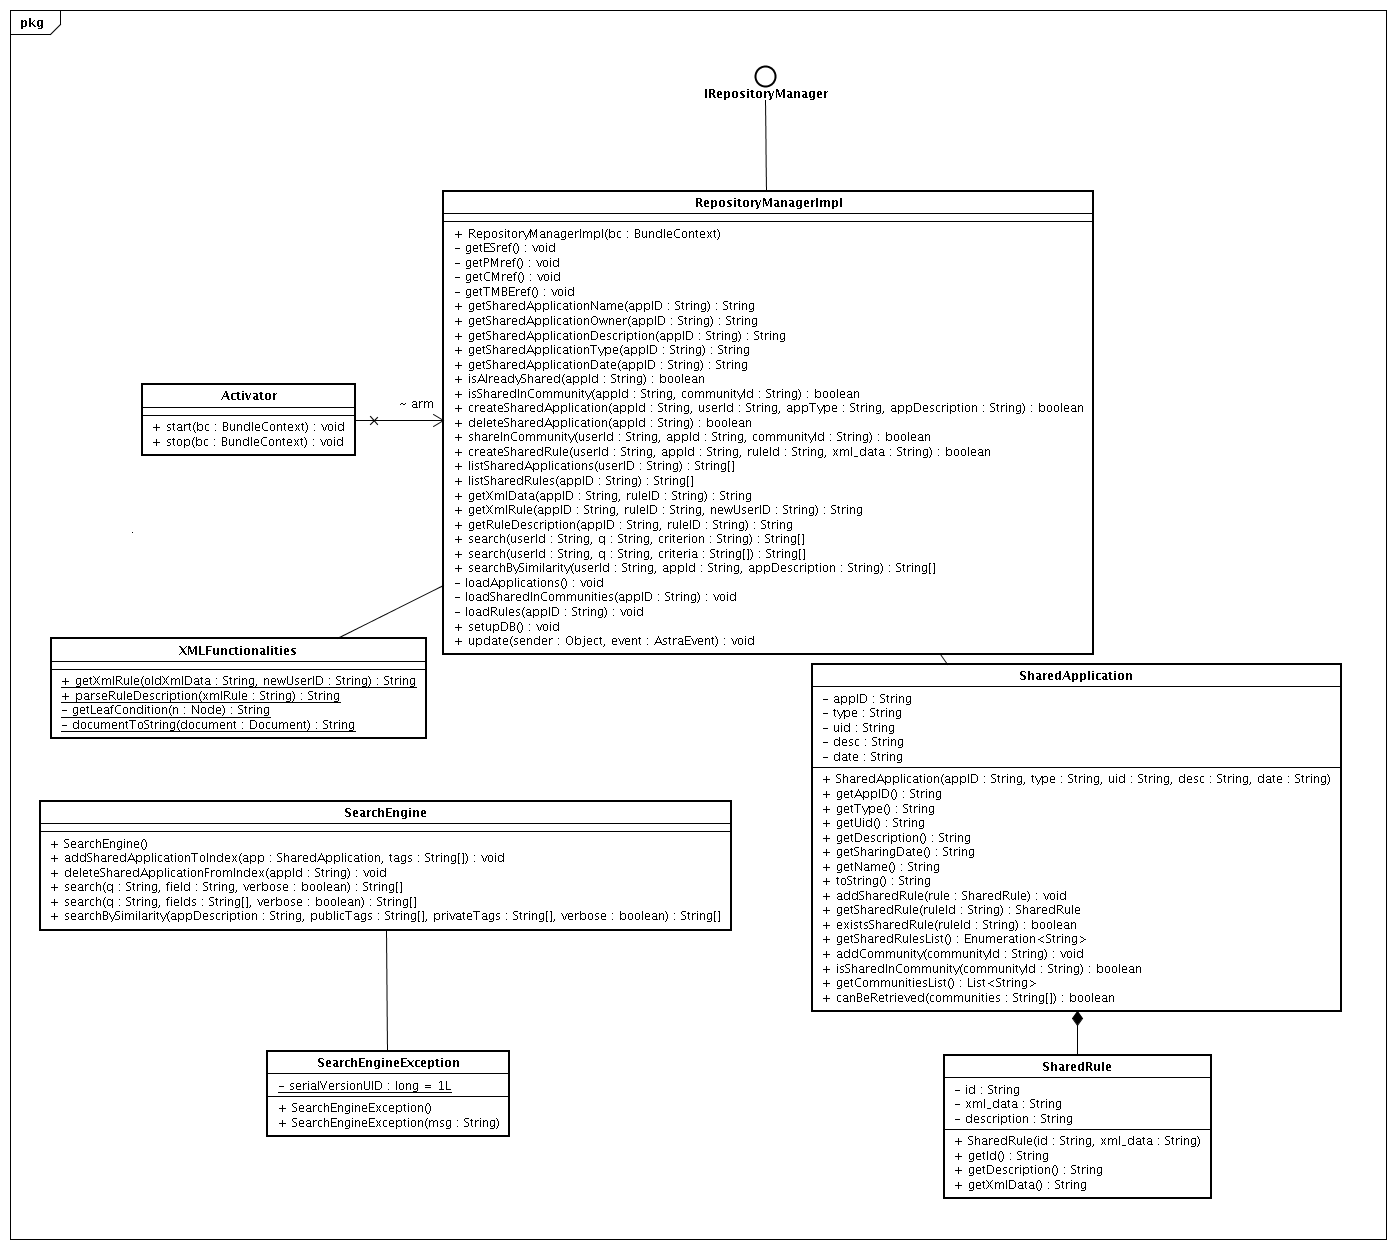
\includegraphics[scale=0.31]{diagrams/RepositoryManagerClassDiagram.png}
  \caption{\label{img:rm-cd}RepositoryManager (class diagram)}
 \end{center}
\end{figure}

\subsubsection{Storage system}

Finally, we needed to design a database model for \verb|RepositoryManager|. We
designed it taking into account the following relationships:

\begin{itemize}
  \item An user owns (has shared) \verb|0..n| applications in the repository.
  \item A shared application has \verb|1..n| shared rules.
  \item A shared application is visible for \verb|1..n| communities.
  \item A community has \verb|0..n| shared applications.
  \item A shared application has \verb|0..n| tags.
\end{itemize}

The Figure \ref{img:rm-db-model} shows a database diagram with all the
necessary tables and the relationships between them which were previously
enumerated.


\begin{figure}[h!]
 \begin{center}
 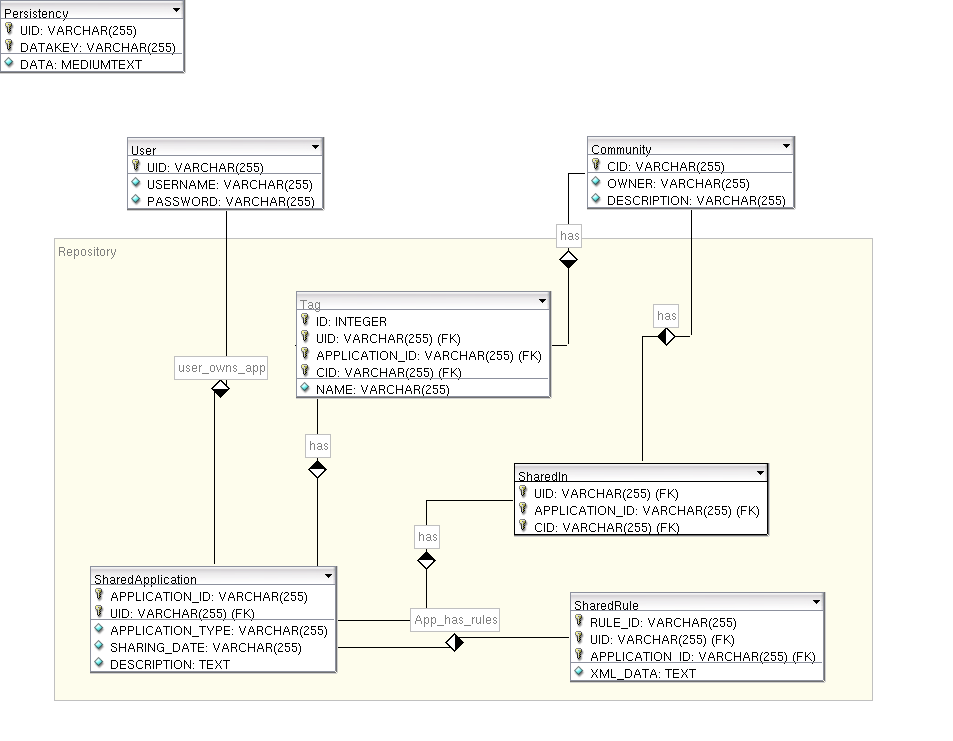
\includegraphics[scale=0.4]{diagrams/RepositoryManagerDBModel.png}
  \caption{\label{img:rm-db-model}RepositoryManager (database model)}
 \end{center}
\end{figure}

It is also important to remark that in order to increase the performance in
querying, the repository keeps also a copy in memory of all the
information about the applications and the rules stored. This
information is stored in hash tables that are synchronized with the data in the
database.
\newline
This decision introduces as a drawback the need of duplicating the number of
create and delete operations (which have to be executed in memory and in the
database) and arises the need of establishing synchronization mechanisms to have
consistent copies in both sides. But considering that most of the operations are
to retrieve information (i.e.: all the needed operations for searching or
getting an application) the global performance also increases.


%%%%%%%%%%%%%%% TagManagerBackEnd %%%%%%%%%%%%%%%%%%%%%%%%%

\subsection{TagManagerBackEnd}
\label{subsec:tmbe-design}

As it was explained in Section \ref{subsec:bundles-design} we decided to divide
the tags management into two components: \verb|TagManagerBackEnd| and
\verb|TagManagerNode| (which will be explained in Section
\ref{subsec:tmn-design}).
\newline
\verb|TagManagerBackEnd| is the bundle that manages the public and community
tags. It is executed in the Backend, and it possess an interface to make its
services available to the rest of the bundles in ASTRA. 
The initial version of the code was based on the code for a tagging system under
the project Ubicollab\footnote{Ubiquitous Collaboration: is an open source
project aiming at implementing a platform for mobile communities developed at
NTNU (http://ubicollab.idi.ntnu.no).} by Christian Laverton, which is licensed
under an Apache License (version 2.0). It was first adapted for ASTRA, and 
extended afterwards.
\newline
In this section we will explain the process we followed to carry on its design, 
taking a similar approach to the one we took to design \verb|RepositoryManager|
(Section \ref{subsec:repository-design}).


\subsubsection{Connection with other bundles}
\label{subsubsec:connections-tmbe}

The first step consisted of defining the relationship between
\verb|TagManagerBackEnd| and the rest of the bundles in ASTRA.

Taking into account the requirements stated in Section \ref{sec:requirements}
and the analysis performed in Section \ref{subsec:tags-use-cases}, we needed to
make use of the services of the following bundles:

\begin{itemize}
  \item \verb|CommunityManager|: Necessary to retrieve information about the
  relationship between users, their communities and the tags. I.e.: to
  make available certain tag taking into account the scope in terms of 
  visibility of the user.
  \item \verb|EventsManager|: Necessary to give feedback of the events produced
  in it. I.e: to inform other bundles that a tag has been added.
  \item \verb|PersistencyManager|: Necessary to store permanently all the data
  into the database. Using its services, we assure the robustness of the system.
\end{itemize}

The Figure \ref{img:tmbe-components} shows graphically the relationship between
\verb|TagManagerBackEnd| and the rest of components through its interfaces.

\begin{figure}[h!]
 \begin{center}
 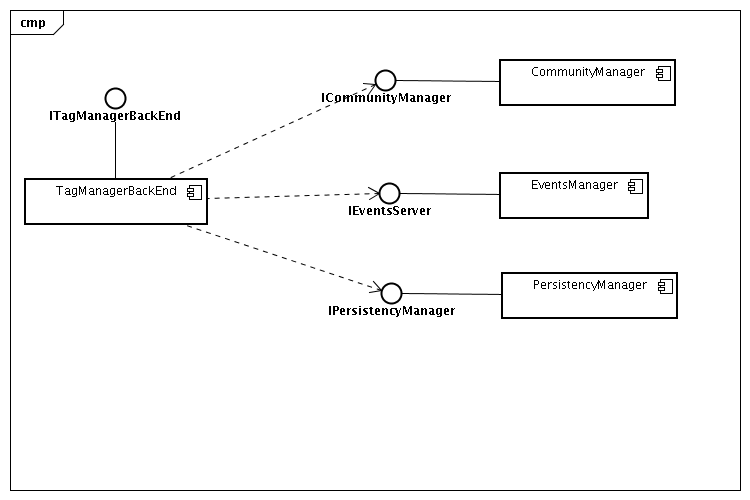
\includegraphics[scale=0.4]{diagrams/TagManagerBackEndComponentsDiagram.png}
  \caption{\label{img:tmbe-components}TagManagerBackEnd (components diagram)}
 \end{center}
\end{figure}

\subsubsection{Interface definition}
\label{subsubsec:tmbe-interface-definition}

The next step consisted of defining its interface. The Tables
\ref{table:tmbe-interface-1} and \ref{table:tmbe-interface-2} summarize the
methods offered by the final version of \verb|TagManagerBackEnd|.

%%tables with repository inteface
%%% Tables for tmbe interface %%%%
\begin{table}[h!]
	\small
    \begin{center}
		\begin{tabular}{||r|l|l||}
        
        %%%%%%%% Begin method %%%%%%%%%%%%%%%%%%
		\hline \hline
		\multicolumn{3}{||c||}{\bfseries{addTag (overloaded)}} \\
		\hline
		\hline 
		\multicolumn{3}{||l||}{Description: Creates a public tag.} \\
		\hline \hline
			Parameter & Type & Description \\
		\hline \hline
			name & String & Tag name. \\
			appId & String & Application identifier in the standard ASTRA format. \\
			userId & String & Identifier of the user who tags the application. \\
		\hline \hline
		\multicolumn{3}{||l||}{Returns: Boolean, true if the operation was successful,
		false otherwise.} \\ \hline \hline
		%%%%%%%%%%%% End method %%%%%%%%%%%%%%%%%%%%%%
		
		%%%%%%%% Begin method %%%%%%%%%%%%%%%%%%
		\hline \hline
		\multicolumn{3}{||c||}{\bfseries{addTag (overloaded)}} \\
		\hline
		\hline 
		\multicolumn{3}{||l||}{Description: Creates a tag only visible for that
		community.} \\ \hline \hline
			Parameter & Type & Description \\
		\hline \hline
			name & String & Tag name. \\
			appId & String & Application identifier in the standard ASTRA format. \\
			userId & String & Identifier of the user who tags the application. \\
			communityId & String & Community identifier. \\
		\hline \hline
		\multicolumn{3}{||l||}{Returns: Boolean, true if the operation was successful,
		false otherwise.} \\ \hline \hline
		%%%%%%%%%%%% End method %%%%%%%%%%%%%%%%%%%%%%


		%%%%%%%% Begin method %%%%%%%%%%%%%%%%%%
		\hline \hline
		\multicolumn{3}{||c||}{\bfseries{getTags}} \\
		\hline
		\hline 
		\multicolumn{3}{||l||}{Description: Returns a list of public tags for the
		given application.} \\ 
		\hline \hline 
			Parameter & Type & Description \\
		\hline \hline
			appId & String & Application identifier in the standard ASTRA format. \\
			limit & Integer & Limit on number of results returned. \\ \hline \hline
		\multicolumn{3}{||l||}{Returns: String array, list of public tags for the
		given application.} \\
		\hline
		\hline
		%%%%%%%%%%%% End method %%%%%%%%%%%%%%%%%%%%%%	
		
		
				%%%%%%%% Begin method %%%%%%%%%%%%%%%%%%
		\hline \hline
		\multicolumn{3}{||c||}{\bfseries{getTagsByCommunity}} \\
		\hline
		\hline 
		\multicolumn{3}{||l||}{Description: Returns a list of public tags for the
		given application and community.} \\ 
		\hline \hline 
			Parameter & Type & Description \\
		\hline \hline
			appId & String & Application identifier in the standard ASTRA format. \\
			limit & Integer & Limit on number of results returned. \\
			communityId & String & Community identifier. \\
		\hline \hline
		\multicolumn{3}{||l||}{Returns: String array, list of public tags for the
		given application and community.} \\
		\hline
		\hline
		%%%%%%%%%%%% End method %%%%%%%%%%%%%%%%%%%%%%	
		
		\end{tabular}
		\caption{\label{table:tmbe-interface-1} TagManagerBackEnd interface}
	\end{center}
\end{table}

\begin{table}[h!]
	\small
    \begin{center}
		\begin{tabular}{||r|l|l||}
        
       
		%%%%%%%% Begin method %%%%%%%%%%%%%%%%%%
		\hline \hline
		\multicolumn{3}{||c||}{\bfseries{getTagsByApplication}} \\
		\hline
		\hline 
		\multicolumn{3}{||l||}{Description: Returns a list of tags associated to 
		the application	which are public} \\ 
		\multicolumn{3}{||l||}{or visible for that user (because he belongs to
		that community).} \\ \hline \hline 
			Parameter & Type & Description \\
		\hline \hline
			appId & String & Application identifier in the standard ASTRA format. \\
			userId & String & User identifier. \\
			limit & Integer & Limit on number of results returned. \\
		\hline \hline
		\multicolumn{3}{||l||}{Returns: String array, list of visible tags for this
		user associated to the given application.}
		\\
		\hline
		\hline
		%%%%%%%%%%%% End method %%%%%%%%%%%%%%%%%%%%%%	
		
		
				%%%%%%%% Begin method %%%%%%%%%%%%%%%%%%
		\hline \hline
		\multicolumn{3}{||c||}{\bfseries{deleteTag (overloaded)}} \\
		\hline
		\hline 
		\multicolumn{3}{||l||}{Description: Deletes a public tag.} \\
		\hline \hline
			Parameter & Type & Description \\
		\hline \hline
			name & String & Tag name. \\
			appId & String & Application identifier in the standard ASTRA format. \\
			userId & String & Identifier of the user who tagged the application. \\
		\hline \hline
		\multicolumn{3}{||l||}{Returns: Boolean, true if the operation was successful,
		false otherwise.} \\ \hline \hline
		%%%%%%%%%%%% End method %%%%%%%%%%%%%%%%%%%%%%
		
		%%%%%%%% Begin method %%%%%%%%%%%%%%%%%%
		\hline \hline
		\multicolumn{3}{||c||}{\bfseries{deleteTag (overloaded)}} \\
		\hline
		\hline 
		\multicolumn{3}{||l||}{Description: Deletes a tag for a given community.} \\
		\hline \hline
			Parameter & Type & Description \\
		\hline \hline
			name & String & Tag name. \\
			appId & String & Application identifier in the standard ASTRA format. \\
			userId & String & Identifier of the user who tagged the application. \\
			communityId & String & Community identifier. \\
		\hline \hline
		\multicolumn{3}{||l||}{Returns: Boolean, true if the operation was successful,
		false otherwise.} \\ \hline \hline
		%%%%%%%%%%%% End method %%%%%%%%%%%%%%%%%%%%%%
		
	
		\end{tabular}
		\caption{\label{table:tmbe-interface-2} TagManagerBackEnd interface (II)}
	\end{center}
\end{table}


% 
% \begin{table}[h!]
% 	\small
%     \begin{center}
% 		\begin{tabular}{||r|l|l||}
%         
% 
% 		
% 		\end{tabular}
% 		\caption{\label{table:tmbe-interface-3} Tag Manager Backend interface (III)}
% 	\end{center}
% \end{table}


\clearpage

\subsubsection{Classes definition}
The definition of the classes in this case is simpler than the one explained in
Section \ref{subsec:rm-classes-definition}: the main functionalities are
provided by the class \verb|TagManagerBackEnd|, which implements the methods of
the interface \verb|ITagManagerBackEnd| explained before in
Section \ref{subsubsec:tmbe-interface-definition} and is responsible for the
communication with the bundles.
\newline
The Figure \ref{img:tmbe-cd} shows the class diagram for this bundle.

\begin{figure}[h!]
 \begin{center}
 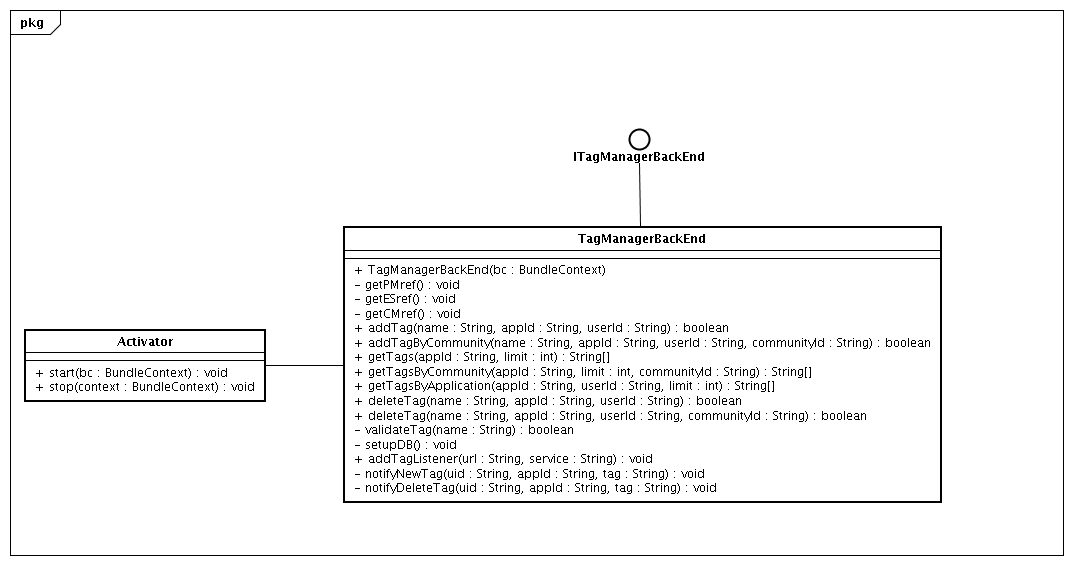
\includegraphics[scale=0.4]{diagrams/TagManagerBackEndClassDiagram.png}
  \caption{\label{img:tmbe-cd}TagManagerBackEnd (class diagram)}
 \end{center}
\end{figure}

\subsubsection{Storage system}
\label{subsubsec:tmbe-storage-system}
The storage system in this case is also simpler: it consists only of one
table as in the code in which was based, allowing back compatibility. 
\newline
The relationships between this table and the repository tables are shown in the
previously explained Figure \ref{img:rm-db-model}.

%%%%%%%%%%%%%%% TagManagerNode %%%%%%%%%%%%%%%%%%%%%%%%%
%\clearpage

\subsection{TagManagerNode}
\label{subsec:tmn-design}

As it was introduced in Section \ref{subsec:tmbe-design}, \verb|TagManagerNode|
is the bundle responsible for the private tags. It is executed in the nodes 
(client side), and it has an interface to offer its services to the rest of 
the bundles in ASTRA.
\newline

In this section we will explain the process we followed to carry on its design, 
taking a similar approach to the one we took previously. \verb|TagManagerNode|
is similar to \verb|TagManagerBackEnd| and, since it has to take care only of
private tags, its design is simpler. Therefore the explanation in this case
will not be so detailed and the reader will be forwarded to previous
subsections when a similar concept arises.

\subsubsection{Connection with other bundles}
\label{subsubsec:connections-tmn}
As is shown in Figure \ref{img:tmn-components}, \verb|TagManagerNode| needs only
the services of \verb|PersistencyManager|, which allow it to store its data
permanently.

\begin{figure}[h!]
 \begin{center}
 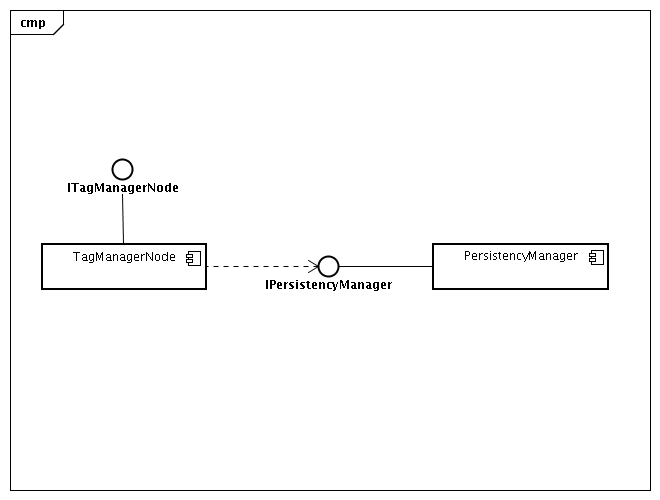
\includegraphics[scale=0.4]{diagrams/TagManagerNodeComponentsDiagram.png}
  \caption{\label{img:tmn-components}TagManagerNode (components diagram)}
 \end{center}
\end{figure}

\subsubsection{Interface definition}
\label{subsubsec:tmn-interface-definition}

\verb|TagManagerNode|`s interface is summarize in Table
\ref{table:tmn-interface}.

%%tables with repository inteface
%%% Tables for tmbe interface %%%%
\begin{table}[h!]
	\small
    \begin{center}
		\begin{tabular}{||r|l|l||}
        
        %%%%%%%% Begin method %%%%%%%%%%%%%%%%%%
		\hline \hline
		\multicolumn{3}{||c||}{\bfseries{addTag}} \\
		\hline
		\hline 
		\multicolumn{3}{||l||}{Description: Creates a new private tag.} \\
		\hline \hline
			Parameter & Type & Description \\
		\hline \hline
			name & String & Tag name. \\
			appId & String & Application identifier in the standard ASTRA format. \\
			userId & String & Identifier of the user who tags the application. \\
		\hline \hline
		\multicolumn{3}{||l||}{Returns: Boolean, true if the operation was successful,
		false otherwise.} \\ \hline \hline
		%%%%%%%%%%%% End method %%%%%%%%%%%%%%%%%%%%%%


		%%%%%%%% Begin method %%%%%%%%%%%%%%%%%%
		\hline \hline
		\multicolumn{3}{||c||}{\bfseries{getTags}} \\
		\hline
		\hline 
		\multicolumn{3}{||l||}{Description: Returns a list of private tags for the
		given application.} \\ 
		\hline \hline 
			Parameter & Type & Description \\
		\hline \hline
			appId & String & Application identifier in the standard ASTRA format. \\
			userId & String & Identifier of the user. \\
			limit & Integer & Limit on number of results returned. \\
		\hline \hline
		\multicolumn{3}{||l||}{Returns: String array, list of private tags for the
		given application.} \\
		\hline
		\hline
		%%%%%%%%%%%% End method %%%%%%%%%%%%%%%%%%%%%%	
		
		%%%%%%%% Begin method %%%%%%%%%%%%%%%%%%
		\hline \hline
		\multicolumn{3}{||c||}{\bfseries{deleteTag}} \\
		\hline
		\hline 
		\multicolumn{3}{||l||}{Description: Deletes a private tag.} \\
		\hline \hline
			Parameter & Type & Description \\
		\hline \hline
			name & String & Tag name. \\
			appId & String & Application identifier in the standard ASTRA format. \\
			userId & String & Identifier of the user who tagged the application. \\
		\hline \hline
		\multicolumn{3}{||l||}{Returns: Boolean, true if the operation was successful,
		false otherwise.} \\ \hline \hline
		%%%%%%%%%%%% End method %%%%%%%%%%%%%%%%%%%%%%

		
		\end{tabular}
		\caption{\label{table:tmn-interface} TagManagerNode interface}
	\end{center}
\end{table}


\clearpage

\subsubsection{Classes definition}
The main functionalities are provided by the class \verb|TagManagerNode| as is
shown in the Figure \ref{img:tmn-cd}.

\begin{figure}[h!]
 \begin{center}
 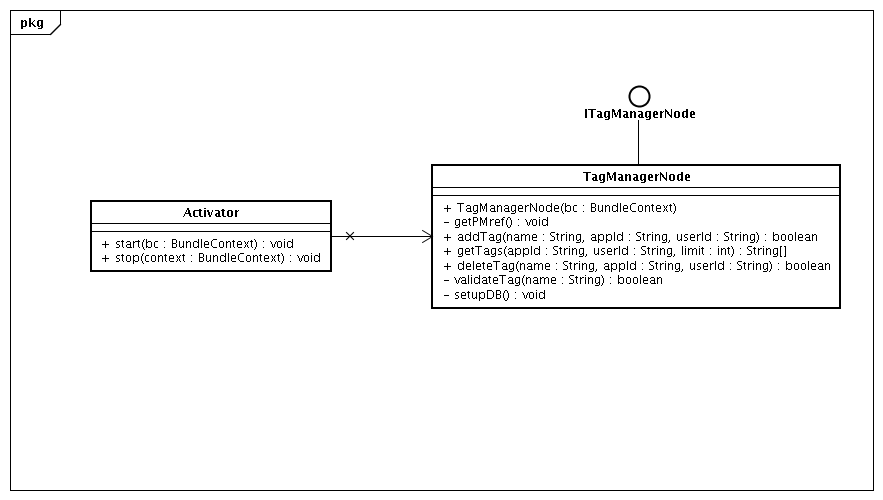
\includegraphics[scale=0.4]{diagrams/TagManagerNodeClassDiagram.png}
  \caption{\label{img:tmn-cd}TagManagerNode (class diagram)}
 \end{center}
\end{figure}

\subsubsection{Storage system}
It consists only of one table, following an schema similar to the one
explained in Section \ref{subsubsec:tmbe-storage-system}.

%%%%%%%%%%%%%%% ApplicationManager %%%%%%%%%%%%%%%%%%%%%%%%%
%\clearpage

\subsection{ApplicationManager}
\label{subsec:am-design}

The last bundle is \verb|ApplicationManager|, which is in charge of the
interaction with the user by offering an intuitive GUI, and the connection with
other ASTRA bundles services based on that interaction. It is executed in the
Node side, and it makes uses of the services offered by the bundles in both
edges: Node (client side) and Backend (server side).
\newline

In this section we will explain the process we followed to carry on its design.
The most important implementation details about this bundle are explained
in Section \ref{sec:implementation}.

\subsubsection{Connection with other bundles}
\label{subsubsec:connections-am}
First we need to analyze the relationship between this bundle and
the rest of bundles in ASTRA.
Taking into account the requirements stated in Section \ref{sec:requirements}
and the analysis performed in Section \ref{sec:use-cases}, it was necessary to
use the services of the following bundles:

\begin{itemize}
  \item Local bundles:
	\begin{itemize}
	  \item \verb|AwarenessApplicationManager|: Necessary to send and receive
	  information about the local applications.
	  \item \verb|AwarenessManager|: Necessary to send and receive information
	  about the local rules.
	  \item \verb|TagManagerNode|: Necessary to manage the private tags.
	  \item \verb|OntologyManager|: Necessary to assist the user in the application
	  adaptation process using ontologies\footnote{This feature is not available
	  in the current version of ASTRA, but \texttt{ApplicationManager} has been
	  prepared to be easily extended. A detailed explanation can be found in Section
	  \ref{subsec:implementation-app-adaptation}.}.
    \end{itemize}
   
   \item Remote bundles:
	\begin{itemize}
	  \item \verb|UserManager|: Necessary to authenticate the users during the
	  logging in process.
	  \item \verb|CommunityManager|: Necessary to retrieve information about the
	  communities joined by the user.
	  \item \verb|TagManagerBackend|: Necessary to manage the public and community
	  tags.
	  \item \verb|RepositoryManager|: Necessary to share and retrieve applications
	  with the rest of the users.
    \end{itemize}
    
\end{itemize}

The Figure \ref{img:am-components} shows graphically the relationship between
\verb|ApplicationManager| and the rest of bundles.

\begin{figure}[h!]
 \begin{center}
 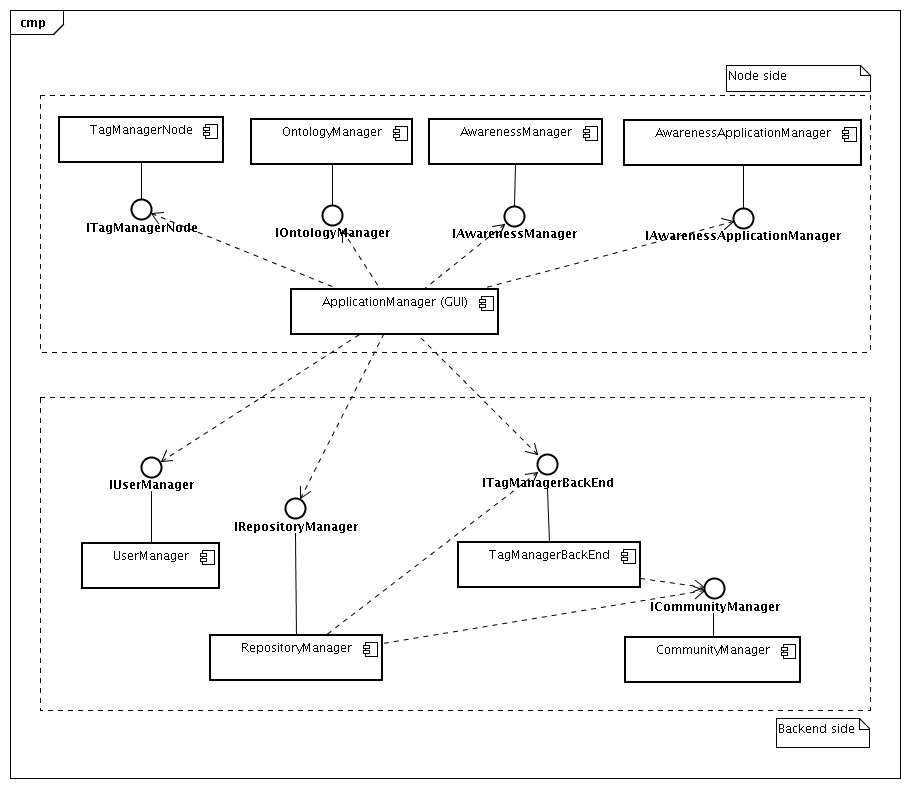
\includegraphics[scale=0.4]{diagrams/ApplicationManagerComponentsDiagram.png}
  \caption{\label{img:am-components}ApplicationManager (components diagram)}
 \end{center}
\end{figure}

\subsubsection{Bundle architecture}
\label{subsub:am-bundle-arch}
In this subsection we will explain briefly the architectural and design
patterns which are implemented by this bundle\footnote{The implementation
details will be stated in Section \ref{sec:implementation}.}, and we will
discuss the reasons why they were chosen.

%%\subsubsubsection{Singleton (design pattern)}

\paragraph{}

\textbf{Singleton (design pattern):}\newline

A design pattern is a description for a commonly recurring structure of communicating
components that solves a general design problem within a
particular context. It provides a scheme for refining the 
components of a software system and the relationships between them.
\newline
In order to implement the MVC architectural pattern, we made use of the
singleton design pattern in the controller. The singleton pattern makes the
class itself responsible for keeping track of its sole instance, ensuring that
no other instance can be created.
\newline
The Figure \ref{img:singleton} shows a singleton general class diagram.


\begin{figure}[h!]
 \begin{center}
 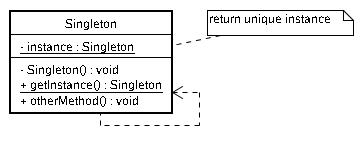
\includegraphics[scale=0.7]{img/singleton.jpg}
  \caption{\label{img:singleton}Singleton design pattern}
 \end{center}
\end{figure}

\paragraph{}

\textbf{MVC (architectural pattern):}\newline

An architectural pattern expresses a fundamental structural organisation or
schema for software systems. It provides a set of predefined subsystems,
specifies their responsibilities, and includes rules and
guidelines for organising the relationships between them.
\newline
\verb|ApplicationManager| implements a MVC (Model-View-Controller) pattern,
which allows us to isolate the business logic from the user interface, permitting one
to be freely modified without affecting the other. The controller collects
user input, the model manipulates application data, and the view presents
results to the user.
\newline
The details about how MVC was implemented in the bundle can be found in Section
\ref{sec:implementation}, and the design of the classes is explained in
Section \ref{subsub:am-classes-definition}.


\subsubsection{Classes definition}
\label{subsub:am-classes-definition}
As we stated in Section \ref{subsub:am-bundle-arch}, \verb|ApplicationManager|
implements a MVC pattern. Therefore the class definition is based on the structural
organization defined for this pattern which we can summarize as follows:

\begin{itemize}
	\item Controller: It is represented by the class
 	 \verb|ApplicationManagerController|, whose job is to contain the interactions
 	 of the user interface components and to interact with other ``business logic''
  	classes. It implements a singleton design pattern.
  	It needs basically to perform two functions:
	\begin{itemize}
  		\item To keep track of the references to the user interface components.
  		\item To provide a set of methods that other components can directly call in
  		their event handler.
    \end{itemize}
    
 	\item Model: It is represented by the class \verb|ApplicationManagerModel|,
 	which contains the ``business logic''. Taking into account the bundle nature
 	of\\ \verb|ApplicationManager|, the ``business logic'' in this case is
 	simpler, summarizing its functions in: 
	\begin{itemize}
  		\item To manage the references to the rest of the bundles.
  		\item To work as an ``stub container'' to make use of the services provided
  		by those.
  		\item To take care of the session data, i.e.: the user identifier.
    \end{itemize}
    Considering we are only go to need a single instance of the model, it also
    implements a singleton pattern\footnote{This is an specific decission for 
   this bundle, and it is not established by the MVC architectural pattern,
   actually in most of the cases the model does not implement it. }.
    
    \item View: It is represented by several classes whose task consist of
    presenting the information to the user. This includes all the classes which
    represent the windows (i.e.: \verb|MainWindow|, \verb|LoginWindow|, etc.)
    and all the necessary classes that extend some of the graphical components (i.e.:
    \verb|TreeRenderer|, \verb|TagListCellRenderer|, etc.)\footnote{These
    classes are ommited in Figure \ref{img:am-cd} in order to make it simpler.}.
\end{itemize}

The Figure \ref{img:am-cd} shows the most important classes that made up this
bundle and the relationships between them.

\begin{figure}[h!]
 \begin{center}
 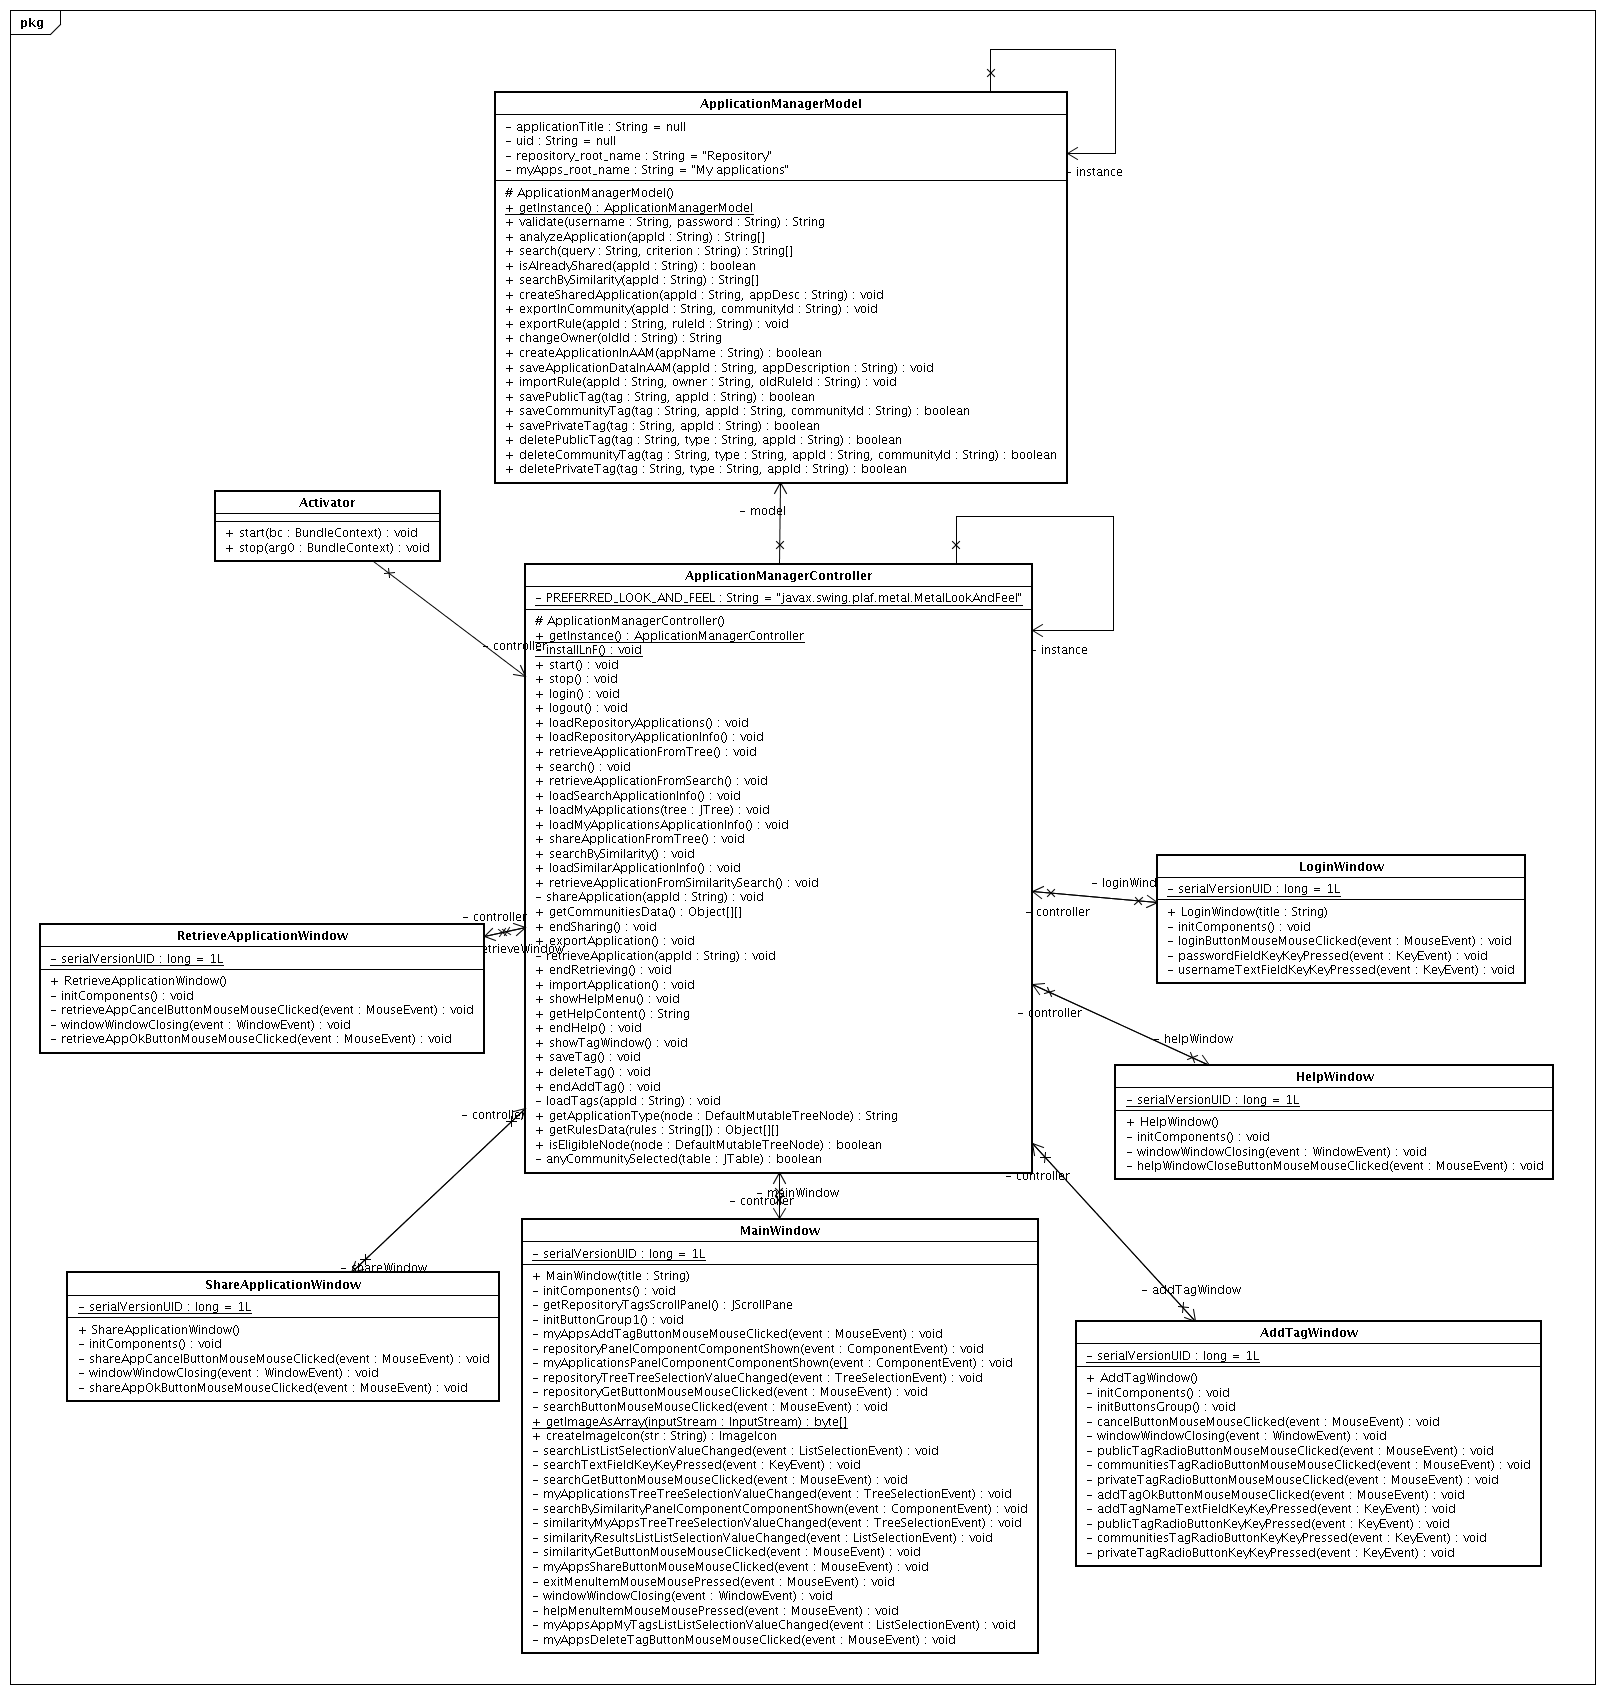
\includegraphics[scale=0.3]{diagrams/ApplicationManagerClassDiagramSmall.png}
  \caption{\label{img:am-cd}ApplicationManager (class diagram)}
 \end{center}
\end{figure}

\subsubsection{GUI design}

Finally, we need to decide the composition of the graphical user interface. It
was divided into the following windows:
\begin{itemize}
  	\item \verb|LoginWindow|: Displays a window where the user can introduce his
  	user name and password.
  	\item \verb|MainWindow|: Displays a window where the user can manage the
  	local and remote applications. It is divided into the following tabs:
	\begin{itemize}
  		\item ``My applications'': 
  			\begin{itemize}
		  		\item It allows the user to browse his applications, see the 
		  		information about them and share them in the repository.
		  		\item It allows the user to manage tags associated to certain 
		  		application.
              \end{itemize}
  		\item ``Repository'': It allows the user to browse the repository, to see
  		information about the applications and to retrieve them.
  		\item ``Search'': It allows the user to perform queries 
  		to look for applications in the repository by different criteria:
  		description, tags, type or any.
  		\item ``Search by similarity'': It allows the user to search
  		applications by choosing one he has in his local space.
    \end{itemize}
    It will also offer a menu tab with options to look up for remote help and
    to log out of the system.
    
    \item \verb|ShareApplicationWindow|: Displays a window where the user can
    customize the parameters of the sharing process: select the communities, 
    select the rules, visualize their description, etc.
    \item \verb|RetrieveApplicationWindow|: Displays a window where the user can
    customize the parameters of the retrieving process: select the rules,
    visualize their description, change the application description, etc.
    \item \verb|AddTagWindow|: Displays a window where the user can tag an
    application and define its visibility.
    \item \verb|HelpWindow|: Displays a window with the help information.
    

\end{itemize}

The user interaction through this GUI is detailed in Section
\ref{sec:user-interaction}.


\clearpage

%%implementation
%%%%%%%%%%%%%%% Implementation %%%%%%%%%%%%%%%%%%%%%%%%%
\section{Implementation}
\label{sec:implementation}

In this section we will describe some of the most important implementation
details that were undertaken during the development phase.

\subsection{Creating and deploying a bundle}
\label{subsec:creating-bundles}

In this section we will enumerate the necessary steps to create
an OSGi bundle and deploy it in the Knopflerfish framework, assuming we have 
already set up the necessary tools (Eclipse, Knopflerfish eclipse plugin, etc)
\footnote{Details about the tools can be found in Section \ref{sec:tools}.}.
It is based on the tutorials in \cite{osgi-tutorial} and \cite{osgi09}.


\subsubsection{Creating the project and the manifest}
First of all, we need to create an OSGi project and ensure that the
\verb|framework.jar| file is imported in the Java Build Path, otherwise we will
not be able to access the OSGi classes and interfaces provided by Knopflerfish.
\newline
One of the differences with respect to a common Java project is the need of
defining a manifest file which contains the description of the bundle. This
manifest is used by the framework to get information about it and to deploy it
successfully. 
As an example we show a simplified version of \verb|RepositoryManager|`s
manifest:

\verbatiminput{code/repository_manifest}

From which we can remark the following attributes:
\begin{itemize}
  \item Export-Packages: It informs the framework which are the classes and
  interfaces offered by this bundle.
  \item Bundle-Classpath: It is necessary to establish all the external
  libraries used by this bundle.
  \item Bundle-Activator: It tells the framework which class is the
  \verb|Activator| class, it is a similar concept to the ``main" class in a
  normal Java application.
  \item Import-Package: It informs the framework about the bundles it needs to
  have access to (only locals). 
\end{itemize}

Appendix \ref{appendix:manifests} contains all the manifests from all the
bundles developed for this project.
\newline
It is also necessary to create an Ant Build file to build the project, but
assuming we are using OSGi Knopflefish plugin for Eclipse, it is created
automatically.

\subsubsection{Creating an activator}

The next step consists of defining the \verb|Activator| class, a class that
implements the \verb|BundleActivator| interface. This interface requires the
implementation of two methods, \verb|start()| and \verb|stop()|, which are used
by the framework to manage the bundle.
The \verb|start()| and \verb|stop()| methods receive a \verb|BundleContext|
object. We have to store this object once we get it and set the reference back
to \verb|null| when the bundle is stopped. That way, the Garbage Collector can
do its work and free unused resources.
\newline
We have also to register the services by calling the \verb|registerService()|
method of the \verb|BundleContext|. It receives three parameters: the first
parameter is the name of the service interface. The second is the service 
implementation. The third parameter can be used to supply additional 
information about the service as key/value pairs.

As an example, Figure \ref{img:repository-activator} shows
\verb|RepositoryManager|'s activator code.

\begin{figure}[h!]
 \begin{center}

 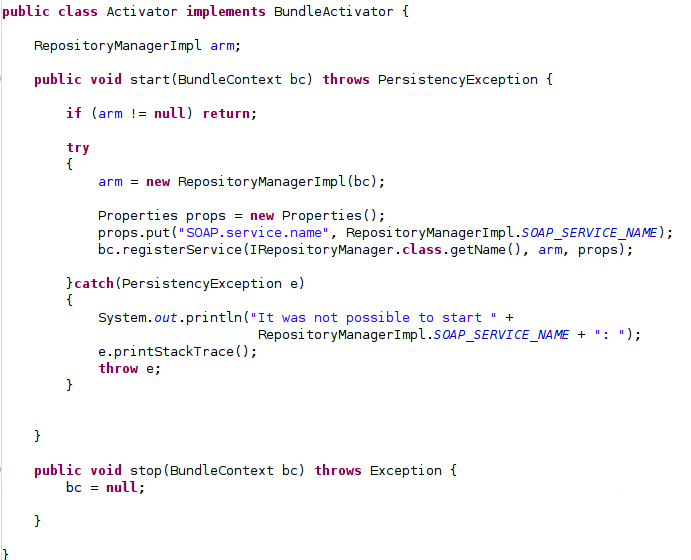
\includegraphics[scale=0.65]{screenshots/repository-activator.png}
  \caption{\label{img:repository-activator}RepositoryManager's activator}
 \end{center}
\end{figure}


\subsubsection{Running the bundles}
Finally, we just need to configure the running configuration. An easy way to
do it is by creating a OSGi run configuration, where we can set the framework,
configure the system properties, etc.
The most delicate part consists of defining the priorities to run the bundles.
This can be problematic for those bundles that make use of other bundles
services when they are run for the first time\footnote{An alternative consists
of creating a \texttt{ServiceTracker} object, but this is out of the scope of
this explanation.}, i.e: the need of \verb|RepositoryManager| to access the
database using \verb|PersistencyManager|'s services when is started for the first time.
\newline
The Figure \ref{img:screenshot-bundles-priorities} shows a screenshot where
the bundles priorities are configured using the OSGi Eclipse plugin.
The configurations for running an ASTRA Node and the ASTRA Backend are
explained in Appendix \ref{appendix:osgi-bundles-config}.

\begin{figure}[h!]
 \begin{center}
 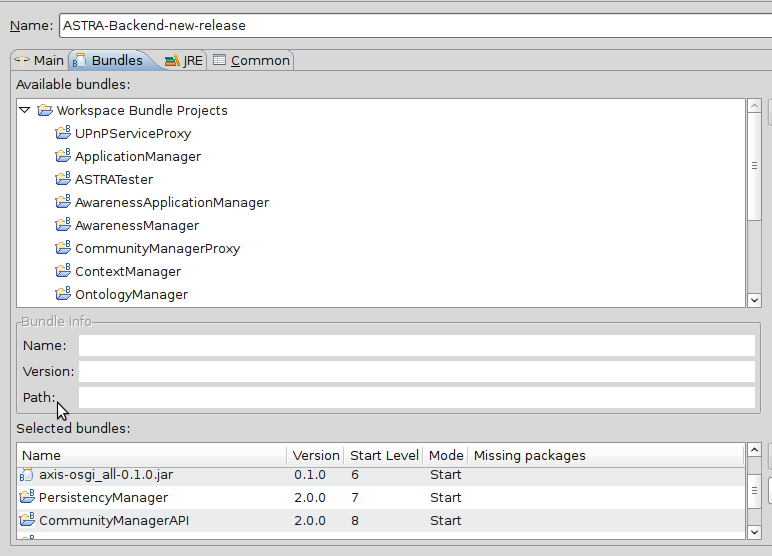
\includegraphics[scale=0.4]{screenshots/back-end-config.png}
  \caption{\label{img:screenshot-bundles-priorities}Bundles priorities
  configuration}
 \end{center}
\end{figure}

After all these steps our bundle can be successfully run and debugged.

\subsection{Implementing MVC in a SWING application}
\label{subsec:implementation-mvc-swing}
In this section we will explain the process carried on to develop the
\verb|ApplicationManager| GUI (whose design was discussed in Section
\ref{subsec:am-design}) following a MVC architectural pattern.
\newline
It is based in some of the ideas explained in \cite{mvc-java} and
\cite{interfaces05}.
\newline
We will summarize it describing the responsibilities of each sub-component:
\begin{itemize}
  \item Controller: It is implemented in a singleton class, which
  	\begin{itemize}
	  \item Keeps track of the user interface components.
	  \item Provides a set of methods that can be called by the events handlers. 
	\end{itemize}
  \item View: All the windows were designed graphically, using a free software
	  plugin for Eclipse called ``Visual Swing 4 Eclipse"\footnote{More details can
	  be found in Section \ref{sec:tools}.}. It offers also facilities to create ``empty"
	  methods that handle the events. This makes the development faster since we
	  only have to:
  	\begin{itemize}
        \item Set the references to the components in the controller.
        \item Establish a relationship between the proper event and the method
        to be called in the controller.
     \end{itemize}
  \item Model: Implements the ``business logic'' that, taking into account the
  SOA nature of the whole project, consists of:
  	\begin{itemize}
        \item Store the user session information and the references to the rest
        of the bundles.
        \item Provides a set of methods with the proper information to be
        consumed by the controller, and make use of the services offered by
        other bundles when necessary.
     \end{itemize}

\end{itemize}

As it was briefly discussed in Section \ref{subsec:am-design}, we assure a
loose coupling relationship between the subcomponents thanks to it.

It is also interesting to remark that the GUI creates background threads to
perform time-consuming tasks, by extending the \verb|SwingWorker| class in
order to keep the GUI responsive \cite{swing-concurrency}. Concretely, threads 
are created for loading the tree hierarchy for remote and local applications.

\subsection{Search engine development}
\label{subsec:implementation-search-engine}
In order to accomplish the requirements related to searching capabilities
(see Section \ref{sec:requirements}) which are captured in Section 
\ref{subsec:searching-use-cases}, we decided to use the open source library
Lucene (see \ref{sec:tech-lucene}).
\newline
Lucene allowed us to provide search capabilities in a really flexible and
powerful way. In this section we will explain the steps we took to create and
integrate the search engine based on this library into \verb|RepositoryManager|
(see Section \ref{subsec:repository-design}).

\subsubsection{Creating the index}
The first step consisted of deciding how the index is going to be created.
\newline
Lucene stores the index in a directory which can be of two different types:
\verb|FSDirectory|, storing the contents in the contents in the file system, or
\verb|RAMDirectory|, storing the contents in memory. Our search engine uses
the latter, since we do not need persistence of this index once 
\verb|RepositoryManager| is stopped, and it offers a better performance.
\newline

Lucene defines a \verb|Document| as the basic unit to be indexed. Every document
is composed of \verb|Fields|, which represent all the information associated to
the \verb|Document|. In our case the notion of what a \verb|Document| is seems
straight: an application, but deciding what information to store about it (the
\verb|Fields|) requires more caution.
\newline
Lucene allows to customize the type of field by configuring how the field is
going to be stored (see Table \ref{table:lucene-storage}) and how is going to
be indexed (see Table \ref{table:lucene-indexation}).

\begin{table}[h!]
	\small
    \begin{center}
		\begin{tabular}{||l|l||}
        
		\hline \hline
		\multicolumn{2}{||c||}{\bfseries{Type of storage}} \\
		\hline
		\hline 
			Type & Description \\
		\hline \hline
			Compress &  Store the original field value in the index in a compressed form.\\
			\hline
			Yes &  Do not store the field value in the index. \\
			\hline
			No & Store the original field value in the index. \\
		\hline \hline

		\end{tabular}
		\caption{\label{table:lucene-storage} Types of field storage options in
		Lucene}
	\end{center}
\end{table}


\begin{table}[h!]
	\small
    \begin{center}
		\begin{tabular}{||l|l|||}
        
		\hline \hline
		\multicolumn{2}{||c||}{\bfseries{Type of indexation}} \\
		\hline
		\hline 
			Type & Description \\
		\hline \hline
			No &  Do not index the field value.\\
			\hline
			Analyzed &  Index the tokens produced by running the field's value through
			an Analyzer.\\
			\hline
			Not Analyzed & Index the field's value without using an Analyzer, so it can
			be searched.\\
			\hline \hline

		\end{tabular}
		\caption{\label{table:lucene-indexation} Types of field indexation in Lucene}
	\end{center}
\end{table}


Taking into account these field types, the Table
\ref{table:lucene-se-fields} summarizes the type of fields we decided to use
and a brief description with the reasons.

\begin{table}[h!]
	\small
    \begin{center}
		\begin{tabular}{||l|l|l|l||}
        
		\hline \hline
		\multicolumn{4}{||c||}{\bfseries{Search engine - fields}} \\
		\hline
		\hline 
			Field & Storage & Indexation & Description\\
		\hline \hline
			App. identifier &  Yes & Not Analyzed & Necessary to return as a result of a
			query.\\
			\hline
			App. description &  Yes & Analyzed & Used for querying.\\
			\hline
			App. type &  Yes & Not Analyzed & Used for querying.\\
			\hline
			App. owner &  Yes & Not Analyzed & Used to filter applications which belong
			to \\
			 & & & the user who is performing the query\\
			\hline
			App. tags &  Yes & Analyzed & Used for querying.\\
			\hline
			\hline

		\end{tabular}
		\caption{\label{table:lucene-se-fields} Fields used by RepositoryManager's
		search engine index}
	\end{center}
\end{table}

The reason why we need to store all the fields is based on the lack of
functionalities to update the document fields in the index. Our search engine
needs to take into account the addition and removal of some fields associated
to a document dynamically (i.e.: the tags which are added or removed), therefore
we need to update that document in the index. The only way to implement this in the
current version of Lucene is by retrieving and deleting the old version of the
document, and creating and indexing the new version of the document (using
information from the old one if it is necessary).

\subsubsection{Querying}
Once we have implemented the index, we have to create a way to perform the
queries.
\newline
Lucene offers us the possibility of querying in one or in many fields
instantiating the classes \verb|QueryParser| or \verb|MultiFieldQueryParser|
respectively. In the case of searching by criteria, the matching is almost
straight as is shown in Table \ref{table:lucene-querying-criteria}.

\begin{table}[h!]
	\small
    \begin{center}
		\begin{tabular}{||l|l|l||}
        
		\hline \hline
		\multicolumn{3}{||c||}{\bfseries{Querying by criteria}} \\
		\hline
		\hline 
			Criterion & Type of query parser & Affected field(s)\\
		\hline \hline
			By description &  \verb|QueryParser| & App. description\\
			\hline
			By tags &  \verb|QueryParser| & App. tags\\
			\hline
			By type &  \verb|QueryParser| & App. type\\
			\hline
			Any &  \verb|MultiFieldQueryParser| & App. description, tags and type\\
			\hline
			\hline

		\end{tabular}
		\caption{\label{table:lucene-querying-criteria} Matching affected fields in
		querying by criteria}
	\end{center}
\end{table}

Thank to this mechanism,  \verb|RepositoryManager| offers a
transparent way to perform the queries easily with the options selected by the
user in the GUI. Therefore we can now transform a sentence in natural language 
into a query in an intuitive way, as is shown in Figure \ref{img:querying}.


\begin{figure}[h!]
 \begin{center}

 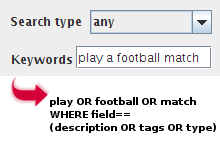
\includegraphics[scale=0.8]{screenshots/query-rich.png}
  \caption{\label{img:querying}Querying the search engine by using the GUI}
 \end{center}
\end{figure}

In the case of the search by similarity a deeper analysis was needed, but after
several tests, which will be detailed in Section \ref{sec:testing}, the queries
are composed by the following data of the application which is going to be
compared:
\begin{itemize}
  \item Application description.
  \item List of public tags.
  \item List of community tags associated to that application (which are visible
  for that user).
\end{itemize}

The query is composed in a similar way as in the one explained in Figure
\ref{img:querying}, and the search is performed on the fields ``description''
and ``tags'' for every application indexed by the search engine.


\subsection{Application adaptation}
\label{subsec:implementation-app-adaptation}
In this section we will explain the details related to the adaptation of an
application retrieved from the repository.
As it will be explained in Section \ref{sec:future-work}, this process aims to
have assistance by inferring using ontologies in the future.
The current state of the implementation performs some automatic changes, but it
still relies on the user's interaction.
\newline
On the other hand, the design and implementation have already taken into account
this possible expansion, so they are already connected with
\verb|OntologyManager| and call its services (which for the moment return a \verb|null| value) through its
interface. Since those methods are not implemented yet, 
\verb|ApplicationManager| offers the possibility of performing this process
manually as is shown in Figure \ref{img:manual-adaptation}.

\begin{figure}[h!]
 \begin{center}

 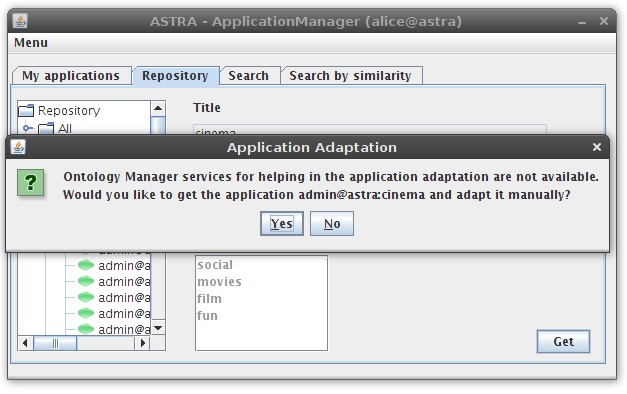
\includegraphics[scale=0.6]{screenshots/manual-adaptation-msg.png}
  \caption{\label{img:manual-adaptation}Offering the alternative of adapting the
  application manually (screenshot)}
 \end{center}
\end{figure}

We can divide the current adaptation functionalities offered in two sets: some
which are performed directly by the user and some that are performed
automatically in a transparent way.
\newline
As is shown in Figure \ref{img:application-adaptation}, the user can currently
modify the description of the application and select the rules before
retrieving the application.

\begin{figure}[h!]
 \begin{center}

 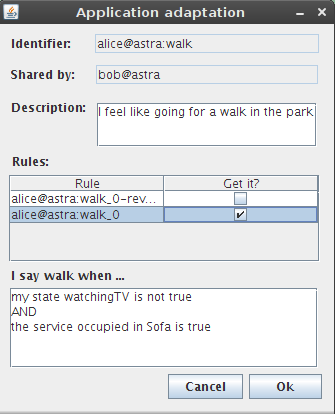
\includegraphics[scale=0.5]{screenshots/application-adaptation-retrieving.png}
  \caption{\label{img:application-adaptation}Application adaptation through the
  GUI (screenshot)}
 \end{center}
\end{figure}

The current automatic changes consist of changing the application and rules
identifiers (see Figure \ref{img:application-adaptation}) and changing
the rules ownership internally. The first one is almost straight, since it is
only necessary to reconstruct the Strings which identify the application or the
rule; but the internal changes in the rules require a deeper analysis.
\newline
The way in that we can access a rule is through an XML file which describes
it\footnote{This XML file is transformed to perform inference by
a subcomponent called \texttt{XMLToClipsParser}, but this is out of the scope of this
explanation.}.

An ASTRA XML rule has the following elements:
\begin{itemize}
  \item \verb|RULES|: The main rule tag that contains the rules. Each
  \verb|RULES| can contain more than one \verb|RULE|.
  \item \verb|RULE|: The tag that contains a single rule. Each rule needs a
  \verb|CONDITION| part and a \verb|RESULT| part.
   \item \verb|RULE_NAME|: The name of the rule.
   \item \verb|CONDITION|: The ``if part'' of the rule.
   \item \verb|TYPE|: The type of condition:
	\begin{itemize}
         \item If \verb|TYPE| is \verb|AND| or \verb|OR| type then it is
         followed by \verb|CONDITION_PART|.
         \item  If the \verb|TYPE| is Service, Awareness or InvokeMessage
         then it is followed by \verb|NAME|, \verb|OPERATOR| and \verb|VALUE|.
    \end{itemize}

   \item \verb|CONDITION_PART|: Defines the parts of a complex condition of an
   \verb|AND| or \verb|OR| type. It always contains two \verb|CONDITION| tags
   that define the two nested conditions.
  \item \verb|NAME|: The name of the variable for the condition.
	\begin{itemize}
      \item  If the \verb|TYPE| is Service, the notation is 
      \verb|<device>@<service>| where the \verb|<device>| is the device that 
      has the \verb|<service>|.
      \item If the \verb|TYPE| is Awareness, it is an intermediate state that 
      is usually described in the Awareness Ontology.
      \item If the \verb|TYPE| is InvokeMessage, it is the name of the
      application that we want to trigger.
    \end{itemize}
  \item \verb|OPERATOR|: The operator that describes the relationship between
	the \verb|NAME| and the \verb|VALUE|. Can be ``eq'', ``neq'', ``gt'', ``ge'',
	``lt'', ``le''. It can be omitted, in which case the default value is ``eq''.
   \item  \verb|VALUE|: The value that is compared with the \verb|NAME| in
   order to validate the condition.
  \item \verb|RESULT|: The ``then part'' of the condition. It is formed in the same
  way as a condition except that no operator is needed.
\end{itemize}


The Figure \ref{img:rule-internal-adaptation} shows an example of a simple XML
rule shared in the repository by user A (Alice), and the same XML rule after
applying the required changes in the ownership once user B (Bob) has retrieved
it. In general, this changes affect:

\begin{figure}[h!]
 \begin{center}

 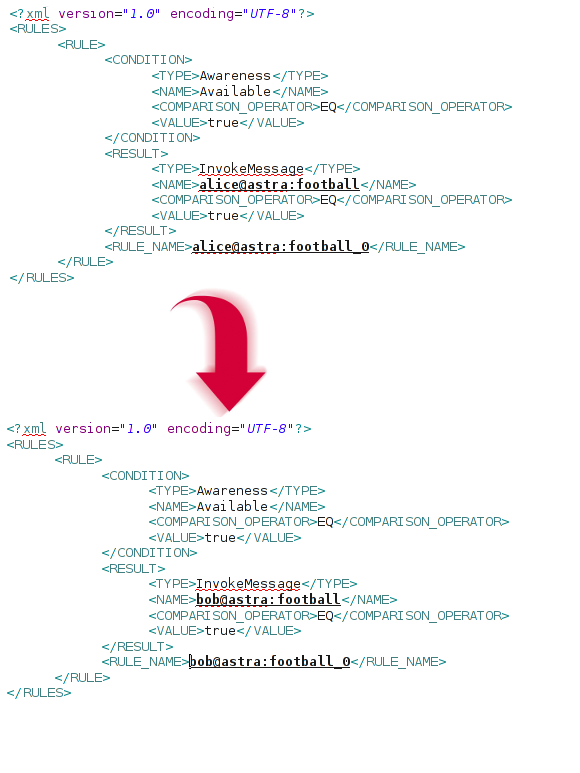
\includegraphics[scale=0.5]{screenshots/rules-transformation.png}
  \caption{\label{img:rule-internal-adaptation}Changes in the internal ownership
  of the rule}
 \end{center}
\end{figure}

\begin{itemize}
  \item All the nodes \verb|NAME| that are children of
  \verb|RESULT|.
  \item The node \verb|RULE_NAME|.
\end{itemize}

A similar approach was taken to create a description  of the rule based on
the XML file (as the one shown in Figure \ref{img:application-adaptation}) in
order to help the user to decide which rules he wants to appropriate. The Figure
\ref{img:rule-tree} shows graphically the way in which we create a human
readable description from a rule while analyzing recursively the
tree which represents the XML rule for an application (i.e.:
\verb|"bob@astra:walk"|).
%\footnote{Some of the nodes that are needed for the construction of the
%description (OPERATOR, VALUE, etc.) are omitted in Figure \ref{img:rule-tree}
%for simplicity reasons.}.

\begin{figure}[h!]
 \begin{center}
 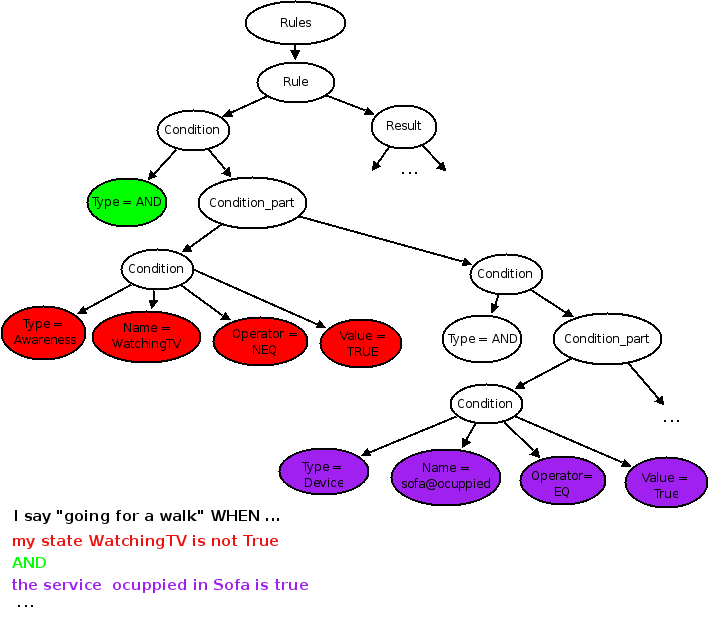
\includegraphics[scale=0.5]{diagrams/rule-tree.png}
  \caption{\label{img:rule-tree} Creating a rule description from an XML
  file}
 \end{center}
\end{figure}

This was implemented using DOM (see Section \ref{subsec:tech-dom}) in the
\verb|RepositoryManager|, and it is accessible for the rest of the bundles by
calling the method \verb|getXMLRule()| and \verb|getRuleDescription()| respectively.






\clearpage

%%user-interaction
%%%%%%%%%%%%%%%%%%%%%%%%% User Interaction %%%%%%%%%%%%%%%%%%%%%%%

\section{User interaction}
\label{sec:user-interaction}

In this section we will explain some of the main functionalities
from the point of view of the user by showing different screenshots.
We will focus on 3 actions: ``tagging and sharing an application'', ``locating an
application'' and ``retrieving and adapting and application from the repository''.

\subsection{Tagging and sharing}
Once the user has successfully logged in the system, he can browse the tree to
see all the information related to his applications in the tab ``My
applications'' as is shown in Figure \ref{img:ui-my-applications}. In order to
distinguish quickly between a focus and a nimbus application (see Section
\ref{subsec:intro-awareness-applications}), the applications are presented with a
different icon (cloud for nimbus, glasses for focus) depending on the type.

\begin{figure}[h!]
 \begin{center}
 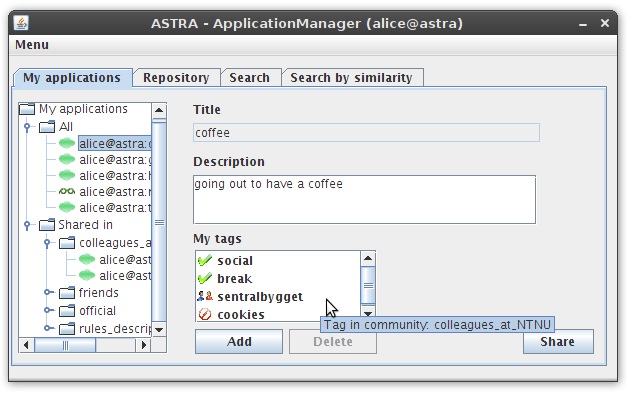
\includegraphics[scale=0.6]{screenshots/ui-my-applications.png}
  \caption{\label{img:ui-my-applications}Interaction with ``My applications''
  (screenshot)}
 \end{center}
\end{figure}

He can manage the tags associated to every application, deleting them or adding
new ones. To make the GUI more intuitive, they are represented with a different
icon depending on the scope as is shown in Figure \ref{img:ui-my-applications}.
There is also a tool tip for every of them, where the user can see the scope
and the community which belongs to in the case of a community tag.
\newline
When the user decides to add a tag, a new window where the user can customize
the scope appears, as is shown in Figure \ref{img:ui-adding-tags}.

\begin{figure}[h!]
 \begin{center}
 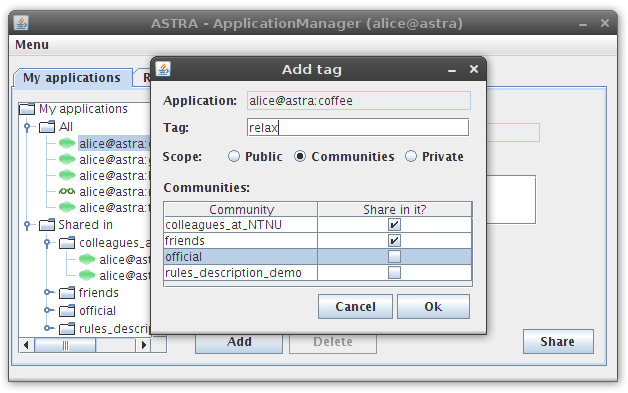
\includegraphics[scale=0.6]{screenshots/ui-adding-tags.png}
  \caption{\label{img:ui-adding-tags}Adding a tag (screenshot)}
 \end{center}
\end{figure}

When the user desires to share an application by pressing the button ``Share'',
another window is displayed. Here he can select the communities where the
application is going to be visible, the rules he wants to share, change the
description, etc. The Figure \ref{img:ui-sharing} shows an screenshot with
that window.

\begin{figure}[h!]
 \begin{center}
 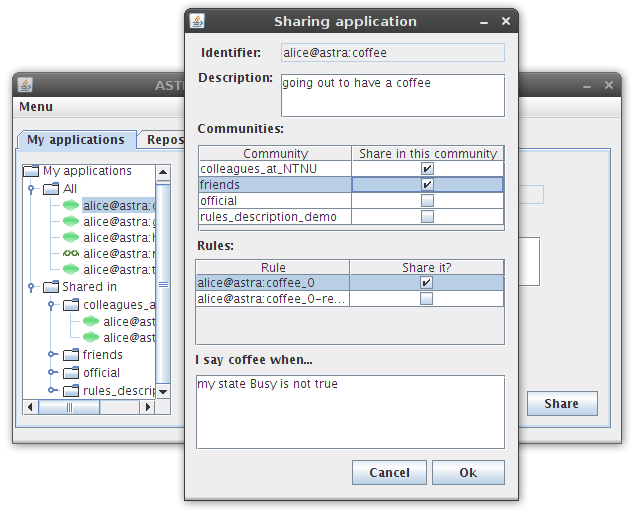
\includegraphics[scale=0.6]{screenshots/ui-sharing.png}
  \caption{\label{img:ui-sharing}Sharing an application (screenshot)}
 \end{center}
\end{figure}


\subsection{Locating an application in the repository}
\label{subsec:ui-locating}
There are three different ways to locate an application in the repository.
The first one is offered in the tab ``Repository'', where the user can browse
the repository and see the main information (description, associated
 visible tags, etc) of the applications which are within his scope. The Figure
 \ref{img:ui-repository} shows the interaction through this tab.
 
\begin{figure}[h!]
 \begin{center}
 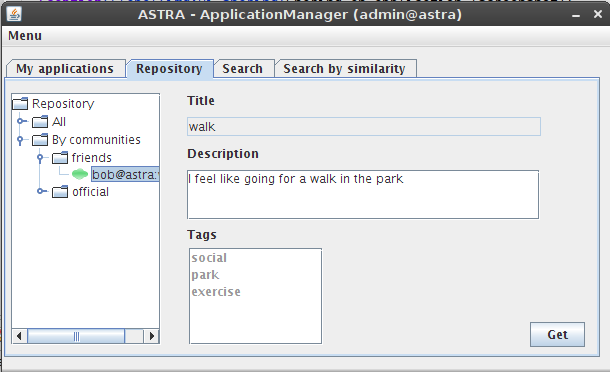
\includegraphics[scale=0.6]{screenshots/ui-repository.png}
  \caption{\label{img:ui-repository}Browsing the repository (screenshot)}
 \end{center}
\end{figure}

The second one is by performing a query, clicking on the tab ``Search''.
Here the user has to select the criteria (any, by description, by tags or by type),
type a query (in natural language, using keywords, etc.) and press the button
``Go!''. Then the results appear in the list below sorted by score, and the
user can see the information related to that results by clicking on them. The
Figure \ref{img:ui-searching-criteria} shows an screenshot of the interaction
through this tab.

\begin{figure}[h!]
 \begin{center}
 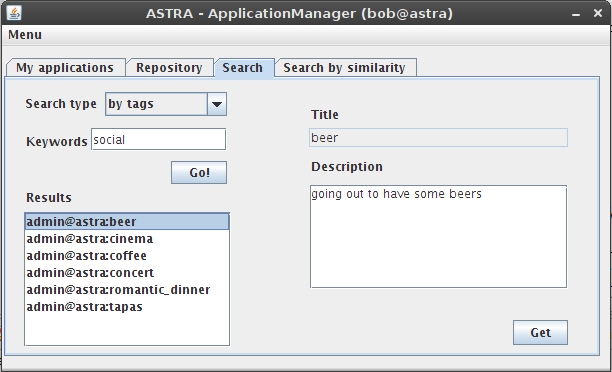
\includegraphics[scale=0.6]{screenshots/ui-searching-criteria.png}
  \caption{\label{img:ui-searching-criteria}Searching an application by  
  criteria (screenshot)}
 \end{center}
\end{figure}

The last option to locate an application is offered in the tab ``Search by
similarity''. Here the user selects one of his applications, and similar
applications sorted by similarity are loaded on the list on the right. Selecting
one of these applications, the user can see the information related to it. The
Figure \ref{img:ui-searching-similarity} shows the interaction through this tab.

\begin{figure}[h!]
 \begin{center}
 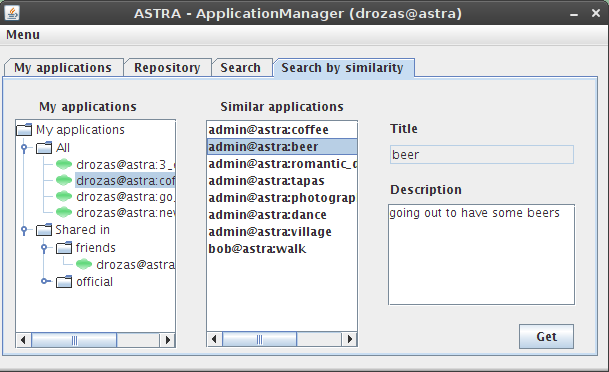
\includegraphics[scale=0.6]{screenshots/ui-searching-similarity.png}
  \caption{\label{img:ui-searching-similarity}Searching an application by 
 similarity (screenshot)}
 \end{center}
\end{figure}

\subsection{Retrieving and adapting an application from the repository}
Once the user has located an application by one of the several ways explained
in Section \ref{subsec:ui-locating} and he decides to get it, a new window
where the user can adapt the application is displayed. He can change the
description and choose the rules he wants to retrieve. The Figure
\ref{img:ui-retrieving} shows an screenshot with the interaction through this
window after having performed a search by similarity.

\begin{figure}[h!]
 \begin{center}
 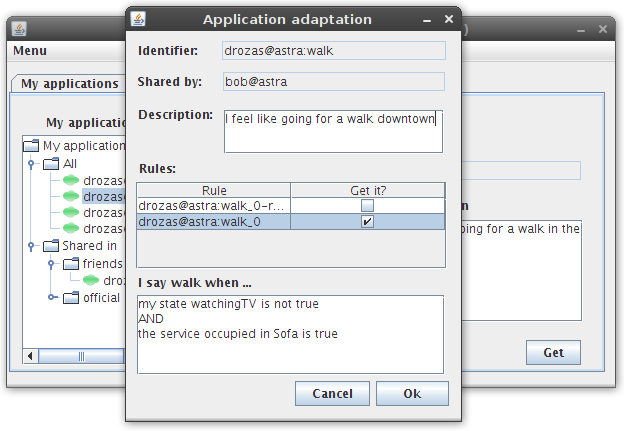
\includegraphics[scale=0.6]{screenshots/ui-retrieving.png}
  \caption{\label{img:ui-retrieving}Retrieving and adapting an application
  from the repository (screenshot)}
 \end{center}
\end{figure}


\clearpage

%%testing
%%%%%%%%%%%%%%% Testing %%%%%%%%%%%%%%%%%%%%%%%%%
\section{Testing}
\label{sec:testing}

In this section we will explain shortly the testing processes we carried on for
this project. As it was explained in Section \ref{section:methodology-spiral}, we have followed a spiral model,
therefore we have performed testing tasks for each iteration (see Table
\ref{table:iterations}).

\subsection{Functionalities verification}

In order to verify the code, we have performed several tests which assure it
works accordingly to its expected behavior. This was performed in a low
level (after finishing every functionality) and in a high level (after every
iteration or before every demonstration). We also stressed on being sure the
application responds correctly in extreme cases like:
\begin{itemize}
  \item Lack of local/remote applications.
  \item No membership in any community.
  \item The network is down.
  \item \ldots
\end{itemize}

There was also a special interest in assuring all the functionalities related
to the visibility of the applications, tags, etc. work properly due to its
straight relationship with privacy protection.

As we will see in Section \ref{subsubsec:testing-users-study}, a preliminary
version (iterations 1 and 2) was successfully tested in an
users evaluation in December 2008, and another users evaluation is scheduled
in October 2009. The current version of the project have passed successfully
all the tests we performed and we can assure it offers all the expected
functionalities described in the previous sections, so it is ready for being
tested in this new users evaluation. The feedback obtained after carrying on
that process will be very valuable to improve it in the future.

\subsection{OS compatibility}

This project has been totally developed under GNU/Linux, concretely under
Ubuntu 8.04 and 8.10.
All the bundles created for this project have been tested successfully under
different versions of GNU/Linux and Windows XP (see Figure
\ref{img:testing-win-linux}) for both subcomponents: ASTRA Node and ASTRA
Backend.

\begin{figure}
 \begin{center}
 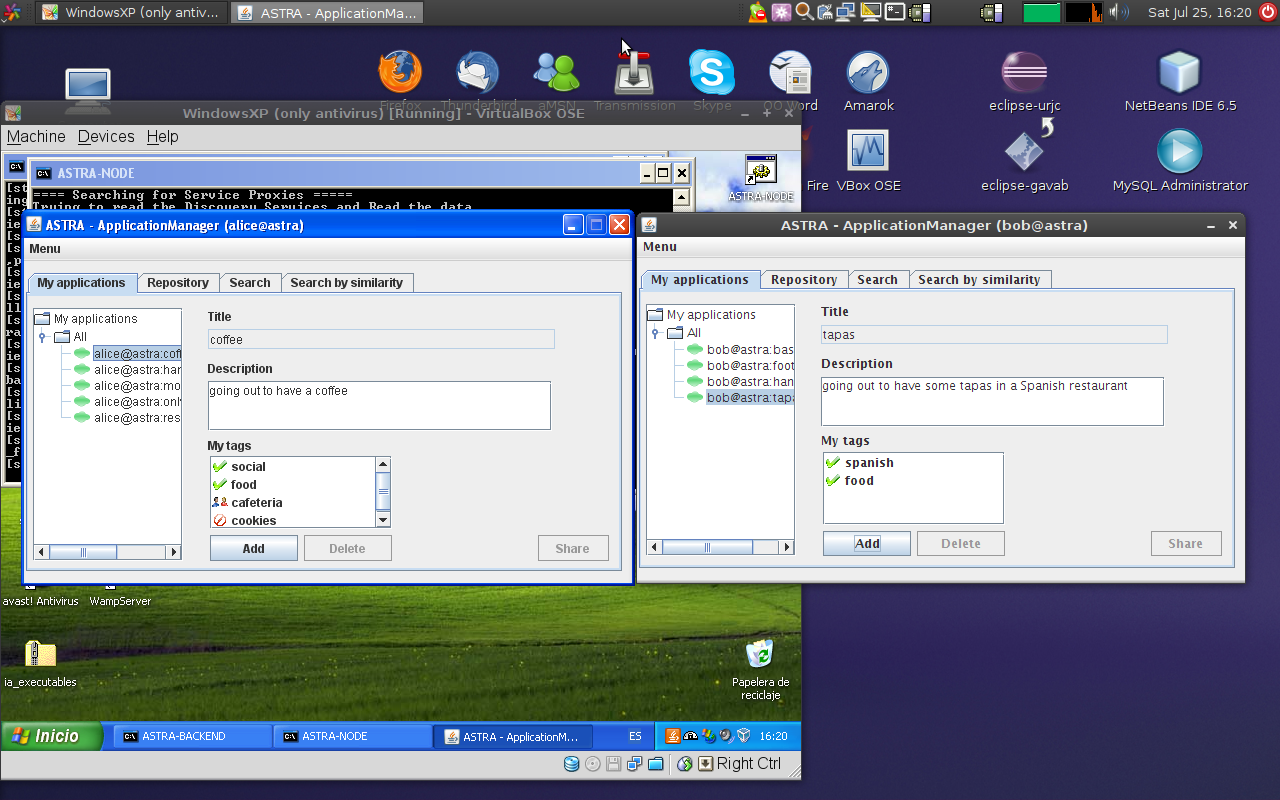
\includegraphics[scale=0.3]{screenshots/am-linux-w32.png}
 \end{center}
 \caption{\label{img:testing-win-linux}ApplicationManager running in GNU/Linux
 and Windows XP simultaneously}
\end{figure}

\subsection{Search engine testing}
\label{subsec:testing-search-engine}

In this section we will explain the process we carried on to evaluate the
search by similarity process. Since the origin of the data is totally
artificial (it was created by only one person) it does not intend to be a real
study, but it explains a possible way to evaluate it once data gathered from a
real set of users will be available.

We created a set of 25 applications, with a description and a set of 4 tags
for each of them. All these applications were under the ownership of an user
called \verb|"admin"| and shared in a community called \verb|"official"|. These
applications were divided into 5 groups: ``Sport'', ``Social'', ``Feelings'',
``Cultural'' and ``Location''. We assumed an application can only belong to one
of this groups to make the measuring process simpler, but this introduces an
error, since the way an application is categorized is subjective and not
exclusive. For example, an application \verb|admin@astra:concert| with
description ``going to a live music concert'' was classified into the group 
``Cultural", but for other people could be in the group ``Social" or even in
both. This will be taken into account when evaluating the results, since we will 
prefer to have a bigger recall even at the expense of loosing precision. The
raw data can be found in the Tables \ref{table:testing-data-sport}, 
\ref{table:testing-data-social}, \ref{table:testing-data-feelings}, 
\ref{table:testing-data-cultural} and \ref{table:testing-data-location} in
Appendix \ref{appendix:testing-search-engine-data}.

We created a new user afterwards that owns 5 applications which are similar (in
description and tags) to one of each of the groups. This will help us to
evaluate if we chose properly the fields to create the query and the fields to
perform the query in (see Section \ref{subsec:implementation-search-engine}).
As we explained in the previously referred section, the results are afterwards
sorted by score (see Appendix \ref{appendix:score-lucene} for more details in
scoring in Lucene).

The measures we took were:

\begin{itemize}
  \item \emph{RD}: Total number of retrieved documents.
  \item \emph{RDR}: Relevant documents retrieved.
  \item \emph{ERD}: Total number of existing relevant documents.
\end{itemize}

With these variables we can calculate the precision and recall percentage:
\[
precision = (RDR/RD)*100
\]

\[
recall = (RDR/ERD)*100
\]
%\\
%${\displaystyle recall = (RDR/ERD)*100}$\




Before taking the measures and perform the calculations, we defined a small set
of testing goals:
\begin{itemize}
  \item The application with the biggest score should be always the one it was
  based on. This acts as a ``control measure'' for the scoring.
  \item We should have a recall of at least 80\%.
  \item We should have a precision of at least 40\%.
\end{itemize}

The reason why we stressed on the recall values at the expense of the
precision is because of the nature of the categorization, as it was explained
before.

The measures and calculations for each application can be found in Tables
\ref{table:testing-results-sport}, \ref{table:testing-results-social},
\ref{table:testing-results-feelings}, \ref{table:testing-results-cultural} and
\ref{table:testing-results-location} in Appendix \ref{appendix:testing-search-engine-data}.

Table \ref{table:testing-summary} summarizes the calculations by groups and on
average.

\begin{table}[h!]
	\small
    \begin{center}
		\begin{tabular}{||c|c|c|c|c|c||}

		\hline \hline
			Group & RD & RDR & ERD & Precision & Recall \\
		\hline \hline
			Sport & 9 & 5 & 5 & 55.56\% & 100\%\\
			\hline
			Social & 10 & 5 & 5 & 50\% & 100\%\\
			\hline
			Feelings & 10 & 5 & 5 & 50\% & 100\%\\
			\hline
			Cultural & 7 & 4 & 5 & 57.14\% & 80\%\\
			\hline
			Location & 10 & 5 & 5 & 50\% & 100\%\\
			\hline
			\hline
			Average & 9.2 & 5 & 5 & 52.54\% & 96\%\\

		\hline \hline

		\end{tabular}
		\caption{\label{table:testing-summary} Summary of the results for search by
		similarity evaluation}
	\end{center}
\end{table}

From this simple evaluation, we can remark:

\begin{itemize}
  \item It satisfies the preliminary testing goals, with a 96\% average in
  recall and 52.54\% average in precision. It also satisfies the ``control
  group'' goal in all the cases.
  \item In most of the cases, the 5 first results belong to the group we were
  expecting (see Appendix \ref{appendix:testing-search-engine-data}). This could
  be useful to establish a threshold in case the precision will decrease too
  much in the future.
  \item When there are false positives, in general all of them belong to
  no more than one or two of the categories (see for instance
  Table \ref{table:testing-results-feelings}). This can be explained because of
  the rigid way we have tagged and categorized the applications in
  contrast with the intrinsic non-exclusive nature of the applications
  categorization.
\end{itemize}

It is important to remark that the data was totally artificial, therefore the
aim of this small evaluation was just assuring the design decisions point to the
right way, and to establish a possible way of measuring in the future.


\subsection{Users evaluation}
\label{subsubsec:testing-users-study}

A preliminary users evaluation after iterations 1 and 2 (see Table
\ref{table:iterations}) was performed at NTNU in Trondheim (Norway) on the 13th
of December 2008. There were 8 participants, all of them exchange students
since those represent one of the main scenarios in ASTRA.
A deep analysis is beyond the scope of this document (detailed information can
be found in \cite{astra-repo}), but we will summarize the most important ideas
and impressions given by the users, and the way we have used this feedback for
developing the current version of the project:

\begin{itemize}
  \item Participants were positive about the idea of sharing and 
 		getting applications.
  \item The notion of community had a good reception, and they evaluated
  positively the visibility in terms of community. This feedback has been taken
  into account in iterations 3 and 4 (i.e.: adding support to browse by
  communities in local and remote applications).
  \item The search functionalities needed to be extended. This is one of the
  main features added in iteration 3 with the integration of a search engine
  into the repository.
  \item Users evaluate very positively the possibility of having public and
  community tags. Users also pointed the necessity of removing them, which is
  supported in the current version.
  \item Users evaluate positively the introduction of ontologies. For instance
  this can be used to support a better categorization. This issue is part
  of the future work (see Section \ref{sec:future-work}), and the bundles
  developed for this project are already integrated with
  \verb|OntologyManager|'s interface, so they will work once that
  functionalities are implemented in that bundle.
  \item Some privacy issues arise, regarding especially the need of removing
  rules. For instance, an application may have a rule which provides
  information about our location that we do not want to share.
  This has been addressed in the current version, in which we provide mechanisms
  to visualize and adapt the application (i.e.: discard a rule after 
  visualizing its auto-generated description), so the users can handle its
  privacy.
  \item Implementing a search by similarity from a recommended application was
  pointed as an interesting option. This is addressed in the current version.
\end{itemize}

A new users evaluation at NTNU including the work performed during iterations 3
and 4 is scheduled in October 2009, once some other ASTRA components will be
developed, so they can also be tested in the same evaluation.

\clearpage

%%coordination
%%%%%%%%%%%%%%%%%%%%%%%%% Coordination %%%%%%%%%%%%%%%%%%%%%%%

\section{Coordination}
\label{sec:coordination}
In this section we will discuss shortly the mechanisms we used in order to
coordinate with the rest of teams during the realization of this project.
This is specially interesting taking into account the big amount of partners
from several countries which are part of the ASTRA project (see Section
\ref{section:what-is-astra}).

The employed coordination mechanisms are listed and described briefly below:
\begin{itemize}
  \item F2F (Face To Face): I have assisted to F2F meetings with members of
  NTNU and Telenor teams during my stay in Trondheim (Norway) (see Section
  \ref{sec:contribution} to see time references). This is obviously the richest
  communication mechanism, and it was specially interesting for the requirements
  elicitation processes. This has also been the main coordination mechanism with
  my supervisor at URJC during my stay in Madrid (Spain).
  \item Teleconferences: I have had weekly teleconference meetings with NTNU,
  Telenor and CTI members. This has been a very useful mechanism to coordinate 
  the work in team, to discuss the state of the project, to share ideas, etc.
  \item Wiki: We have used a wiki website (http://www.astra-project.net/wiki)
  to coordinate the bundles development process. This has been a very useful
  tool to be aware about other teams bundles and to produce a good
  documentation.
  \item Subversion: The project code is hosted in a SVN server at NTNU \\ 
  (http://basar.idi.ntnu.no/svn/astra/). This has been a really useful tool to
  coordinate the development process, since it allows us to avoid and resolve 
  possible code conflicts, and to have revisions for every code updating.
  \item E-mail: This supposes the main asynchronous communication mechanism,
  and it has been very useful to coordinate with all the members of the team.
  For instance, it has been used to report bugs.
\end{itemize}


\clearpage

%%tools
%%%%%%%%%%%%%%%%%%%%%%%%% Tools %%%%%%%%%%%%%%%%%%%%%%%

\section{Tools}
\label{sec:tools}
In this section we will describe briefly the main tools employed for the
achievement of this project. 
There have been a personal interest in the use of free or open-source software
due to all the advantages that it offers to us. Therefore, all the tools we 
have employed (except Jude, which was used under a freeware license) have a
license of these characteristics.

The list below, summarizes the most important tools employed for this project:

\begin{itemize}
  %\item Ubuntu GNU/Linux, versions 8.04 and 8.10. Free software operating
  %system.
  \item Eclipse 3.4.1 as IDE, including the following plugins (all of them free
  or open source software):
  		\begin{itemize}
            \item Knopflerfish OSGi IDE, version 1.0.16. Plugin to help in OSGi
            bundles development (see Section
            \ref{subsubsec:tech-osgi-knopflerfish}).
            \item Subclipse, version 1.4.8. Provides support for Subversion.
            \item Visual Swing, version 0.9. Provides visual GUI design tools.
            \item Textlipse, version 1.3.0. Provides \LaTeX{} support.
          \end{itemize}
   \item Knopflerfish, version 2.3. Open source OSGi service platform.
   \item MySQL, version 5.1. Open source RDBMS (see Section
   \ref{subsec:tech-mysql}).
   \item PHPMyAdmin, version 3.2. Open source tool to handle MySQL
   administration through a web interface.
   \item Apache, version 2.2. Free software HTTP server.
   \item Dia, version 0.96. Free software program to draw diagrams.
   \item Jude Community, version 5.4.1. Freeware program for UML modeling.
   \item VirtualBox, version 3.0.2. Open source virtualizer for x86 hardware.
   \item GIMP, version 2.6. Free software for image manipulation.
          
\end{itemize}

\clearpage


%%Conclusions
\chapter{Conclusions}
\label{chap:conclusions}
This chapter concludes the report discussing briefly the fulfillment of the
objectives and discussing my personal contribution to ASTRA. Some
suggestions about future work are also included, as well as a personal evaluation.


\section{Achieved goals}
\label{sec:goals}

In this report we have detailed the process carried on to develop and integrate
a set of bundles to manage awareness applications into ASTRA, including
functionalities for sharing, tagging, locating, appropriating and adapting the
applications. A new GUI to access this functionalities has also been
developed, demonstrating the flexibility of the ASTRA SOA (see Section 
\ref{subsubsec:tech-astra-soa}). All the work has been carried on stressing its
extensibility, so new functionalities can be easily added in the future as we
will see in Section \ref{sec:future-work}. Therefore, we can conclude we have 
successfully fulfilled all the goals stated in Chapter \ref{chap:objectives}.

\section{Contribution}
\label{sec:contribution}
In this section we will discuss briefly my contribution to ASTRA, including
also time references.

I started my contribution to ASTRA as part of my summer job for the IDI
(Institutt for Datateknikk og Informasjonsvitenskap) at NTNU during
the summer of 2008 (July-September). In this period I participated in the
analysis, design, implementation and testing of the first version of 
\verb|RepositoryManager|, \verb|TagManagerBackend| and \verb|TagManagerNode|.
During this term, I was working in close cooperation with another member of the
NTNU ASTRA team, and we followed a extreme-programming model (see Section 
\ref{section:methodology-spiral}). The work performed during this period made 
up iterations 1 and 2 (see Table \ref{table:iterations}).

I resumed my collaboration with ASTRA project in February 2009. During this
period I worked in the analysis, design, implementation and testing of\\
\verb|ApplicationManager| and in the extension of the functionalities of
other bundles: including search capabilities in \verb|RepositoryManager| and
the addition of new functionalities in \verb|TagManagerBackend| and
\verb|TagManagerNode|, etc. This made up iterations 3 and 4 (see Table
\ref{table:iterations}). Most of the work was developed during my stay in
Madrid, and I coordinated using the mechanisms explained in Section
\ref{sec:coordination}. I also had the opportunity to come back to Norway to
work in ASTRA during one month and a half during the summer, which was
extremely useful to elicit and implement the last requirements and conclude 
successfully the project.


\section{Future work}
\label{sec:future-work}
In this section we present a set of possible enhancements for this project:

\begin{itemize}
  \item The parameters for the searching by similarity process can be adjusted
  to increase its recall and precision once an evaluation process similar to
  the one explained in Section \ref{subsec:testing-search-engine} with real
  user data is carried on.
  \item The use of ontologies for helping in the application adaptation process
  can be included once the implementation of the necessary methods in the\\
  \verb|OntologyManager| is finished. \verb|ApplicationManager| is already
  prepared to make use of its services.
  \item An extension of the GUI could be performed, adding the possibility of
  publishing applications, join communities, rules edition, etc.
  \item New browsing methods (by owner, by tags, etc.) could be developed, to
  allow the user localize applications in new ways.
\end{itemize} 


\section{Personal evaluation}
My work for ASTRA has been one of the most enriching experiences of my
career. I have had the opportunity to work in a real researching project and
to collaborate with teams from several countries. It has also been really
enriching in technological terms, since I have increased my knowledge about all
the technologies discussed in Chapter \ref{chap:methodology}.
It has been really important in personal terms as well, since this experience
allowed me to discover my passion for researching.
Therefore, I will always be grateful for having had the opportunity to 
be part of this project.



%%Appendixes

\appendix
\chapter{Document scoring in Lucene}
\label{appendix:score-lucene}
\phantomsection 

In this section we will explain the scoring process employed in our search
engine. We use the class \verb|org.apache.lucene.search.DefaultSimilarity|
provided by the Lucene library. 
This explanation is based on \cite{lucene-scoring-explanation} and
\cite{lucene-scoring-formula}.

Lucene scoring uses a combination of the Vector Space Model (VSM) of
Information Retrieval and the Boolean model to determine how relevant a given 
Document is to a User's query. In general, the idea behind the VSM is the more 
times a query term appears in a document relative to the number of times the
term  appears in all the documents in the collection, the more relevant that 
document is to the query. It uses the Boolean model to first narrow down the 
documents that need to be scored based on the use of boolean logic in the Query
specification. Lucene also adds some capabilities and refinements onto this
model to support boolean and fuzzy searching, but it essentially remains a VSM 
based system at the heart.

The score for a query \emph{q} in a document \emph{d} is computed as follows:

\[
score(q,d) =  coord(q,d) * queryNorm(q)  * \sum_{t\phantom{i}in\phantom{i}
q}(tf(t\phantom{i}in\phantom{i}d) * idf(t)^2 * t.getBoost() * norm(t,d))
\]

where
\begin{itemize}
  \item \emph{tf(t in d)} correlates to the term's frequency, defined as the
  number of times term \emph{t} appears in the currently scored document
  \emph{d}. Documents that have more occurrences of a given term receive a
  higher score. The default computation for \emph{tf(t in d)} in
  \verb|DefaultSimilarity| is: \[ tf(t\phantom{i}in\phantom{i}d) =
  frequency^{1/2}\]
  \item \emph{idf(t)} stands for Inverse Document Frequency. This value
  correlates to the inverse of \emph{docFreq} (the number of documents in which
  the term \emph{t} appears). This means rarer terms give higher contribution to
  the total score. The default computation for \emph{idf(t}) in
  \verb|DefaultSimilarity| is: \[ idf(t)= 1 + \log (numdocs/(docFreq + 1)) \]
  \item \emph{coord(q,d)} is a score factor based on how many of the query  
  terms are found in the specified document. Typically, a document that
  contains more of the query's terms will receive a higher score than another 
  document with fewer query terms. This is a search time factor computed
  at search time.
  \item \emph{queryNorm(q)} is a normalizing factor used to make scores between
  queries comparable. This factor does not affect document ranking (since all 
  ranked documents are multiplied by the same factor), but rather just attempts
  to make scores from different queries (or even different indexes) comparable.
  This is a search time factor computed at search time. The default computation
  in \verb|DefaultSimilarity| is: \[ queryNorm(q)= 1 /sumOfSquareWeights^{1/2}\]
  \\ The sum of squared weights (of the query terms) is computed by the query
  \verb|Weight object|. For example, a boolean query  computes this value as: \[
  sumOfSquareWeights= q.getBoost()^2 *  \sum_{t\phantom{i}in\phantom{i}
q}((idf(t) * t.getBoost())^2)\]
  \item \emph{t.getBoost()} is a search time boost of term \emph{t} in the query
   \emph{q} as specified in the query text.
  \item \emph{norm(t,d)} encapsulates a few (indexing time) boost and length
  factors:
  		\begin{itemize}
            \item \emph{Document boost}, set by calling \verb|doc.setBoost()| 
            before adding the document to the index. 
            \item \emph{Field boost}, set by calling \verb|field.setBoost()|
            before adding the field to a document. 
            \item \emph{lengthNorm(field)}, computed when the document is added
            to the index in accordance with the number of tokens of this field
            in the document, so that shorter fields contribute more to the score. 
            \emph{LengthNorm} is computed by the \verb|Similarity| class in
            effect at indexing.
          \end{itemize}
   When a document is added to the index, all the above factors are
   multiplied. If the document has multiple fields with the same name, all
   their boosts are multiplied together: \[
  norm(t,d)= doc.getBoost() * 
  lengthNorm(field) * \prod_{field\phantom{i}in\phantom{i}
  d\phantom{i}named\phantom{i}as\phantom{i}t}(f.getBoost()) \]
\end{itemize}




\chapter{Search engine - Testing data}
\label{appendix:testing-search-engine-data}
\phantomsection 

In this appendix we detail the data we gathered to perform the evaluation of
the search by similarity offered by the search engine. The analysis of this
data can be found in Section \ref{subsec:testing-search-engine}.

Tables \ref{table:testing-data-sport}, \ref{table:testing-data-social},
\ref{table:testing-data-feelings}, \ref{table:testing-data-cultural} and
\ref{table:testing-data-location} shows the initial set of raw data from which
we began our analysis for each group.

%Sport
\begin{table}[h!]
	\tiny
    \begin{center}
		\begin{tabular}{||l|l|l||}

		\hline \hline
		\multicolumn{3}{||c||}{\bfseries{Sport}} \\
		\hline \hline
			Application identifier & Application description & Tags \\
			\hline \hline
			admin@astra:go\_jogging	& go jogging to the forest & sport, exercise, run,
			fit\\
			\hline
			admin@astra:go\_to\_the\_gym & go to the gym to train & fit, health, sport,
			muscle\\
			\hline
			admin@astra:play\_basketball\_match & play an amateur basketball match &
			health, ball, sport, amateur\\
			\hline
			admin@astra:play\_football & play a football match & ball, sport, goalkeeper,
			offside\\
			\hline
			admin@astra:play\_handball & play a handball match & sport, fun, ball,
			amateur\\
		\hline \hline

		\end{tabular}
		\caption{\label{table:testing-data-sport}Search by similarity evaluation - raw
		data (sport)}
	\end{center}
\end{table} 

%Social
\begin{table}[h!]
	\tiny
    \begin{center}
		\begin{tabular}{||l|l|l||}

		\hline \hline
		\multicolumn{3}{||c||}{\bfseries{Social}} \\
		\hline \hline
			Application identifier & Application description & Tags \\
			\hline \hline
			admin@astra:beer & going out to have some beers & beer, fun, social,
			friends\\
			\hline
			admin@astra:tapas & go to a Spanish restaurant to have some tapas
			& restaurant, food, spain, social\\
			\hline
			admin@astra:coffee & going to have a coffee & break, social, relax, talk\\
			\hline
			admin@astra:romantic\_dinner & going to an Italian restaurant to have a
			romantic dinner & restaurant, meal, food, social\\
			\hline
			admin@astra:dance & going out to dance in some disco & party, friends, beer,
			fun\\
		\hline \hline

		\end{tabular}
		\caption{\label{table:testing-data-social}Search by similarity evaluation -
		raw data (social)}
	\end{center}
\end{table} 

%Feelings
\begin{table}[h!]
	\tiny
    \begin{center}
		\begin{tabular}{||l|l|l||}

		\hline \hline
		\multicolumn{3}{||c||}{\bfseries{Feelings}} \\
		\hline \hline
			Application identifier & Application description & Tags \\
			\hline \hline
			admin@astra:happy & I am really happy & feeling, nice, love, great\\
			\hline
			admin@astra:hating\_you & I think of you, and I am really angry & angry,
			hate, feelings, furious\\
			\hline
			admin@astra:missing\_you & I am missing you so much & love, nostalgy,
			feeling, lovely\\
			\hline
			admin@astra:sad	& I feel sad & lonely, feeling, terrible, nostalgy\\
			\hline
			admin@astra:thinking\_of\_you &	I miss you and I am thinking of you & love,
			nostalgy, feeling, hug\\
		\hline \hline

		\end{tabular}
		\caption{\label{table:testing-data-feelings}Search by similarity evaluation -
		raw data (feelings)}
	\end{center}
\end{table} 


%Cultural
\begin{table}[h!]
	\tiny
    \begin{center}
		\begin{tabular}{||l|l|l||}

		\hline \hline
		\multicolumn{3}{||c||}{\bfseries{Cultural}} \\
		\hline \hline
			Application identifier & Application description & Tags \\
			\hline \hline
			admin@astra:go\_sightseeing & go sightseeing in our city & tourism, cultural,
			guide, museum\\
			\hline
			admin@astra:museum & go to a museum & paintings, history, cultural, tourism\\
			\hline
			admin@astra:photography\_exposition & going to that new photography
			exposition & pics, cultural, sightseeing, camera\\
			\hline
			admin@astra:concert & go to a live music concert & music, fun, social, rock\\
			\hline
			admin@astra:cinema & watch a movie in the cinema & movies, social, film,
			fun\\

		\hline \hline

		\end{tabular}
		\caption{\label{table:testing-data-cultural}Search by similarity evaluation -
		raw data (cultural)}
	\end{center}
\end{table} 

%Location
\begin{table}[h!]
	\tiny
    \begin{center}
		\begin{tabular}{||l|l|l||}

		\hline \hline
		\multicolumn{3}{||c||}{\bfseries{Location}} \\
		\hline \hline
			Application identifier & Application description & Tags \\
			\hline \hline
			admin@astra:girlfriend\_home & I am at my girlfriend home & busy, home,
			place, gf\\
			\hline
			admin@astra:home & I am at home	& place, home, location, safe\\
			\hline
			admin@astra:my\_parents & I am at my parents home & family, mother, father,
			place\\
			\hline
			admin@astra:office & I am at work, in my office & work, job, place, office\\
			\hline
			admin@astra:village & I am going to be in my mother village & parents,
			mother, place, rustic\\
		\hline \hline

		\end{tabular}
		\caption{\label{table:testing-data-location}Search by similarity evaluation -
		raw data (location)}
	\end{center}
\end{table} 

Tables \ref{table:testing-results-sport}, \ref{table:testing-results-social},
\ref{table:testing-results-feelings}, \ref{table:testing-results-cultural} and
\ref{table:testing-results-location} shows the results returned by the search
engine ordered by scored (as they are presented to the user).
The application we compare to was based on similar information
to the one indicated in \textbf{bold} (``control measure'', see Section 
\ref{subsec:testing-search-engine}). Applications in \textit{italic} are the
ones which belong to the same group we are testing (true positives).
An analysis of these results can be found in Table \ref{table:testing-summary}.

%Sports
\begin{table}[h!]
	\tiny
    \begin{center}
		\begin{tabular}{||l|l|l||}

		\hline \hline
		\multicolumn{3}{||c||}{\bfseries{Sports}} \\
		\hline \hline
			Application returned & Field & Score \\
			\hline \hline
			\textit{\textbf{admin@astra:play\_handball}} & Sport & 2.18\\
			\hline
			\textit{admin@astra:play\_basketball\_match}&	Sport	&	1.4	\\	
			\hline
			\textit{admin@astra:play\_football}	&	Sport	&	0.64	\\
			\hline
			admin@astra:beer	&	Social	&	0.03	\\
			\hline
			admin@astra:cinema	&	Cultural	&	0.03	\\
			\hline
			admin@astra:concert	&	Cultural	&	0.03	\\
			\hline
			admin@astra:dance	&	Social	&	0.03	\\
			\hline
			\textit{admin@astra:go\_jogging} &	Sport	&	0.03	\\
			\hline
			\textit{admin@astra:go\_to\_the\_gym}	&	Sport	&	0.03	\\
		\hline \hline

		\end{tabular}
		\caption{\label{table:testing-results-sport}Search by similarity evaluation
		- results for group ``Sport''}
	\end{center}
\end{table} 

%Social
\begin{table}[h!]
	\tiny
    \begin{center}
		\begin{tabular}{||l|l|l||}

		\hline \hline
		\multicolumn{3}{||c||}{\bfseries{Social}} \\
		\hline \hline
			Application returned & Field & Score \\
			\hline \hline
			\textit{\textbf{admin@astra:beer}}	&	Social	&	2.21	\\
			\hline
			\textit{admin@astra:dance}	&	Social	&	0.99	\\
			\hline
			\textit{admin@astra:coffee}	&	Social	&	0.19	\\
			\hline
			\textit{admin@astra:tapas}	&	Social	&	0.18	\\
			\hline
			\textit{admin@astra:romantic\_dinner}	&	Social	&	0.15	\\
			\hline
			admin@astra:cinema	&	Cultural	&	0.08	\\
			\hline
			admin@astra:concert	&	Cultural	&	0.08	\\
			\hline			
			admin@astra:play\_handball	&	Sport	&	0.02	\\
			\hline
			admin@astra:photography\_exposition	&	Cultural	&	0.02	\\
			\hline
			admin@astra:village	&	Location	&	0.01	\\

		\hline \hline

		\end{tabular}
		\caption{\label{table:testing-results-social}Search by similarity evaluation
		- results for group ``Social''}
	\end{center}
\end{table} 


%Feelings
\begin{table}[h!]
	\tiny
    \begin{center}
		\begin{tabular}{||l|l|l||}

		\hline \hline
		\multicolumn{3}{||c||}{\bfseries{Feelings}} \\
		\hline \hline
			Application returned & Field & Score \\
			\hline \hline
			
			\textit{\textbf{admin@astra:thinking\_of\_you}}	&	Feelings	&	2.4	\\
			\hline
			\textit{admin@astra:missing\_you}	&	Feelings	&	0.92	\\
			\hline
			\textit{admin@astra:happy}	&	Feelings	&	0.34	\\
			\hline
			\textit{admin@astra:hating\_you}	&	Feelings	&	0.3	\\
			\hline
			\textit{admin@astra:sad}	&	Feelings	&	0.23	\\
			\hline
			admin@astra:home	&	Location	&	0.08	\\
			\hline
			admin@astra:girlfriend\_home	&	Location	&	0.07	\\
			\hline
			admin@astra:my\_parents	&	Location	&	0.07	\\
			\hline
			admin@astra:office	&	Location	&	0.07	\\
			\hline
			admin@astra:village	&	Location	&	0.06	\\


		\hline \hline

		\end{tabular}
		\caption{\label{table:testing-results-feelings}Search by similarity evaluation
		- results for group ``Feelings''}
	\end{center}
\end{table} 

%Cultural
\begin{table}[h!]
	\tiny
    \begin{center}
		\begin{tabular}{||l|l|l||}

		\hline \hline
		\multicolumn{3}{||c||}{\bfseries{Cultural}} \\
		\hline \hline
			Application returned & Field & Score \\
			\hline \hline

			\textit{\textbf{admin@astra:museum}}	&	Cultural	&	1.68	\\
			\hline
			\textit{admin@astra:go\_sightseeing}	&	Cultural	&	0.91	\\
			\hline
			\textit{admin@astra:photography\_exposition}	&	Cultural	&	0.05	\\
			\hline
			\textit{admin@astra:concert}	&	Cultural	&	0.03	\\
			\hline
			admin@astra:go\_jogging	&	Sport	&	0.03	\\
			\hline
			admin@astra:go\_to\_the\_gym	&	Sport	&	0.03	\\
			\hline
			admin@astra:tapas	&	Social	&	0.02	\\


		\hline \hline

		\end{tabular}
		\caption{\label{table:testing-results-cultural}Search by similarity evaluation
		- results for group ``Cultural''}
	\end{center}
\end{table} 

%Location
\begin{table}[h!]
	\tiny
    \begin{center}
		\begin{tabular}{||l|l|l||}

		\hline \hline
		\multicolumn{3}{||c||}{\bfseries{Location}} \\
		\hline \hline
			Application returned & Field & Score \\
			\hline \hline
			
			\textit{\textbf{admin@astra:home}}	&	Location	&	2.88	\\
			\hline
			\textit{admin@astra:girlfriend\_home}	&	Location	&	1.28	\\
			\hline
			\textit{admin@astra:my\_parents}	&	Location	&	0.73	\\
			\hline
			\textit{admin@astra:office}	&	Location	&	0.2	\\
			\hline
			\textit{admin@astra:village}	&	Location	&	0.19	\\
			\hline
			admin@astra:happy	&	Feelings	&	0.08	\\
			\hline
			admin@astra:hating\_you	&	Feelings	&	0.07	\\
			\hline
			admin@astra:thinking\_of\_you	&	Feelings	&	0.07	\\
			\hline
			admin@astra:missing\_you	&	Feelings	&	0.06	\\
			\hline
			admin@astra:sad	&	Feelings	&	0.02	\\

		\hline \hline

		\end{tabular}
		\caption{\label{table:testing-results-location}Search by similarity evaluation
		- results for group ``Location''}
	\end{center}
\end{table} 




\chapter{Bundles manifests}
\label{appendix:manifests}
\phantomsection 

In this appendix we list the manifests of the bundles developed for this
project. The meaning of the most relevant attributes is explained in Section
\ref{subsec:creating-bundles}.

\section{RepositoryManager's manifest}

\begin{verbatim}

Manifest-Version: 1.0
Export-Package: eu.ist.astra.rm,eu.ist.astra.rm.impl
Bundle-Vendor: IST ASTRA
Bundle-ClassPath: ., lib/lucene-2_4_1_svn.jar
Bundle-Version: 2.0.0
Bundle-Name: RepositoryManager
Bundle-Activator: eu.ist.astra.rm.impl.Activator
Bundle-Description: Repository Manager bundle which manages the sharing
process in the back-end
Import-Package: 
	org.osgi.framework, 
	eu.ist.astra.persistency, 
	eu.ist.astra.cm, eu.ist.astra.tmbe, 
	eu.ist.astra.em, eu.ist.astra.em.events, 
	javax.xml.parsers;resolution:=optional, 
	javax.xml.transform;resolution:=optional, 
	javax.xml.transform.dom;resolution:=optional, 
	javax.xml.transform.stream;resolution:=optional, 
	org.w3c.dom;resolution:=optional
Bundle-SymbolicName: RepositoryManager

\end{verbatim}

\section{TagManagerBackEnd's manifest}

\begin{verbatim}

Manifest-Version: 1.0
Export-Package: eu.ist.astra.tmbe
Bundle-Vendor: Astra
Bundle-ClassPath: .
Bundle-Version: 2.0.0
Bundle-Name: TagManagerBackEnd
Bundle-Activator: eu.ist.astra.tmbe.impl.Activator
Bundle-SymbolicName: TagManagerBackEnd
Import-Package: 
	org.osgi.framework, 
	eu.ist.astra.persistency, 
	eu.ist.astra.cm, eu.ist.astra.em, 
	eu.ist.astra.em.events
Bundle-ManifestVersion: 2



\end{verbatim}

\section{TagManagerNode's manifest}

\begin{verbatim}

Manifest-Version: 1.0
Export-Package: eu.ist.astra.tmn
Bundle-Vendor: Astra
Bundle-ClassPath: .
Bundle-Version: 2.0.0
Bundle-Name: TagManagerNode
Bundle-Activator: eu.ist.astra.tmn.impl.Activator
Bundle-SymbolicName: TagManagerNode
Import-Package: 
	org.osgi.framework, 
	eu.ist.astra.persistency

\end{verbatim}

\section{ApplicationManager's manifest}

\begin{verbatim}

Manifest-Version: 1.0
Bundle-Vendor: ASTRA
Bundle-ClassPath: ., lib/grouplayout.jar
Bundle-Version: 2.0.0
Bundle-Name: ApplicationManager
Bundle-Activator: eu.ist.astra.am.Activator
Bundle-SymbolicName: ApplicationManager
Import-Package: 
	org.osgi.framework, 
	eu.ist.astra.aam, eu.ist.astra.rfm,
	eu.ist.astra.rfm.proxies, eu.ist.astra.ontologymanager.api, 
	eu.ist.astra.tmn,
	eu.ist.astra.awarenessmanager, 
	javax.swing;resolution:=optional,
	javax.swing.event;resolution:=optional, 
	javax.swing.table;resolution:=optional,
	javax.swing.text;resolution:=optional, 
	javax.swing.text.html;resolution:=optional, 
	javax.swing.tree;resolution:=optional

\end{verbatim}
\chapter{OSGi bundles configuration}
\label{appendix:osgi-bundles-config}
\phantomsection 


In this appendix we present the configuration files (\verb|xinit.args|)
necessary to run the bundles in the proper order for the Backend and the Nodes.
These configuration files are read by the framework on the startup process, so
it can decides which bundles to start and in which order.

\section{OSGi - Backend configuration}

\begin{verbatim}
#
# Generated from template.xargs Knopflerfish release 2.0.1
# drozas: the latest information about the configuration can
# be found at: http://www.astra-project.net/wiki/ConfigurationForBackEnd
#
# load common properties
-xargs props.xargs

# Prefix for searching for bundle URLs from console or command line
-Dorg.knopflerfish.gosg.jars=file:ASTRA/
#-Deu.ist.astra.cm.proxy.endpoint=
http://localhost:8080/axis/services/CommunityManager

-init

#extra Initializations for ASTRA
-istart jsdk/jsdk-2.2.jar
-istart log/log_all-2.0.1.jar
-istart cm/cm_all-2.0.0.jar
-istart commons-logging/commons-logging_all-2.0.0.jar
-istart http/http_all-2.0.0.jar
-istart axis-osgi/axis-osgi_all-0.1.0.jar

-istart RemoteFrameworkManager-2.0.0.jar
-istart EventsManager-2.0.0.jar
-istart PersistencyManager-2.0.0.jar
-istart CommunityManagerAPI-2.0.0.jar
-istart UserManager-2.0.0.jar
-istart CommunityManager-2.0.0.jar
-istart AwarenessApplicationManagerBackend-2.0.0.jar
-istart TagManagerBackEnd-2.0.0.jar
-istart RepositoryManager-2.0.0.jar
-launch
\end{verbatim}

\section{OSGi - Node configuration}

\begin{verbatim}
#
# Generated from template.xargs
# Knopflerfish release 2.0.1
#
# drozas: the latest information about the configuration can 
#be found at: http://www.astra-project.net/wiki/ConfigurationForNode
# load common properties
-xargs props.xargs

# Prefix for searching for bundle URLs from console or command line
-Dorg.knopflerfish.gosg.jars=file:ASTRA/
#You may want to change this parameter to refer to another server
-Deu.ist.astra.cm.proxy.endpoint=
http://localhost:8080/axis/services/CommunityManager
-Deu.ist.astra.BackEndAddress=http://localhost:8080/
-Deu.ist.astra.default.user=john@astra

-init

#extra Initializations for ASTRA
-istart jsdk/jsdk-2.2.jar
-istart cm/cm_all-2.0.0.jar
-istart commons-logging/commons-logging_all-2.0.0.jar
-istart http/http_all-2.0.0.jar
-istart axis-osgi/axis-osgi_all-0.1.0.jar
-istart jena_bundle.jar

-istart RemoteFrameworkManager-2.0.0.jar
-istart EventsManager-2.0.0.jar
-istart OntologyManager-2.0.0.jar
-istart PersistencyManager-2.0.0.jar
-istart CommunityManagerAPI-2.0.0.jar
-istart CommunityManagerProxy-2.0.0.jar
-istart UserManagerProxy-2.0.0.jar
-istart UserManagerAPI-2.0.0.jar
-istart AwarenessManager-2.0.0.jar
-istart AwarenessApplicationManager-2.0.0.jar
-istart ServiceProxyManager-2.0.0.jar
-istart UPnPServiceProxy-2.0.0.jar
-istart ContextManager-2.0.0.jar
-istart TagManagerNode-2.0.0.jar
#-istart ASTRATester-2.0.0.jar
-istart ApplicationManager-2.0.0.jar

-launch
\end{verbatim}
%---------------------------------------------------------------------
%\appendix{\rlap{GNU Free Documentation License}}
\chapter{GNU Free Documentation License}
\label{appendix:gfdl}
\phantomsection  % so hyperref creates bookmarks
%%\addcontentsline{toc}{chapter}{GNU Free Documentation License}
%\label{label_fdl}

 \begin{center}

       Version 1.3, 3 November 2008


 Copyright \copyright{} 2000, 2001, 2002, 2007, 2008  Free Software Foundation, Inc.
 
 \bigskip
 
     http://fsf.org/
  
 \bigskip
 
 Everyone is permitted to copy and distribute verbatim copies
 of this license document, but changing it is not allowed.
\end{center}


\begin{center}
{\bf\large Preamble}
\end{center}

The purpose of this License is to make a manual, textbook, or other
functional and useful document ``free'' in the sense of freedom: to
assure everyone the effective freedom to copy and redistribute it,
with or without modifying it, either commercially or noncommercially.
Secondarily, this License preserves for the author and publisher a way
to get credit for their work, while not being considered responsible
for modifications made by others.

This License is a kind of ``copyleft'', which means that derivative
works of the document must themselves be free in the same sense.  It
complements the GNU General Public License, which is a copyleft
license designed for free software.

We have designed this License in order to use it for manuals for free
software, because free software needs free documentation: a free
program should come with manuals providing the same freedoms that the
software does.  But this License is not limited to software manuals;
it can be used for any textual work, regardless of subject matter or
whether it is published as a printed book.  We recommend this License
principally for works whose purpose is instruction or reference.


\begin{center}
{\Large\bf 1. APPLICABILITY AND DEFINITIONS\par}
\phantomsection
\addcontentsline{toc}{section}{1. APPLICABILITY AND DEFINITIONS}
\end{center}

This License applies to any manual or other work, in any medium, that
contains a notice placed by the copyright holder saying it can be
distributed under the terms of this License.  Such a notice grants a
world-wide, royalty-free license, unlimited in duration, to use that
work under the conditions stated herein.  The ``\textbf{Document}'', below,
refers to any such manual or work.  Any member of the public is a
licensee, and is addressed as ``\textbf{you}''.  You accept the license if you
copy, modify or distribute the work in a way requiring permission
under copyright law.

A ``\textbf{Modified Version}'' of the Document means any work containing the
Document or a portion of it, either copied verbatim, or with
modifications and/or translated into another language.

A ``\textbf{Secondary Section}'' is a named appendix or a front-matter section of
the Document that deals exclusively with the relationship of the
publishers or authors of the Document to the Document's overall subject
(or to related matters) and contains nothing that could fall directly
within that overall subject.  (Thus, if the Document is in part a
textbook of mathematics, a Secondary Section may not explain any
mathematics.)  The relationship could be a matter of historical
connection with the subject or with related matters, or of legal,
commercial, philosophical, ethical or political position regarding
them.

The ``\textbf{Invariant Sections}'' are certain Secondary Sections whose titles
are designated, as being those of Invariant Sections, in the notice
that says that the Document is released under this License.  If a
section does not fit the above definition of Secondary then it is not
allowed to be designated as Invariant.  The Document may contain zero
Invariant Sections.  If the Document does not identify any Invariant
Sections then there are none.

The ``\textbf{Cover Texts}'' are certain short passages of text that are listed,
as Front-Cover Texts or Back-Cover Texts, in the notice that says that
the Document is released under this License.  A Front-Cover Text may
be at most 5 words, and a Back-Cover Text may be at most 25 words.

A ``\textbf{Transparent}'' copy of the Document means a machine-readable copy,
represented in a format whose specification is available to the
general public, that is suitable for revising the document
straightforwardly with generic text editors or (for images composed of
pixels) generic paint programs or (for drawings) some widely available
drawing editor, and that is suitable for input to text formatters or
for automatic translation to a variety of formats suitable for input
to text formatters.  A copy made in an otherwise Transparent file
format whose markup, or absence of markup, has been arranged to thwart
or discourage subsequent modification by readers is not Transparent.
An image format is not Transparent if used for any substantial amount
of text.  A copy that is not ``Transparent'' is called ``\textbf{Opaque}''.

Examples of suitable formats for Transparent copies include plain
ASCII without markup, Texinfo input format, LaTeX input format, SGML
or XML using a publicly available DTD, and standard-conforming simple
HTML, PostScript or PDF designed for human modification.  Examples of
transparent image formats include PNG, XCF and JPG.  Opaque formats
include proprietary formats that can be read and edited only by
proprietary word processors, SGML or XML for which the DTD and/or
processing tools are not generally available, and the
machine-generated HTML, PostScript or PDF produced by some word
processors for output purposes only.

The ``\textbf{Title Page}'' means, for a printed book, the title page itself,
plus such following pages as are needed to hold, legibly, the material
this License requires to appear in the title page.  For works in
formats which do not have any title page as such, ``Title Page'' means
the text near the most prominent appearance of the work's title,
preceding the beginning of the body of the text.

The ``\textbf{publisher}'' means any person or entity that distributes
copies of the Document to the public.

A section ``\textbf{Entitled XYZ}'' means a named subunit of the Document whose
title either is precisely XYZ or contains XYZ in parentheses following
text that translates XYZ in another language.  (Here XYZ stands for a
specific section name mentioned below, such as ``\textbf{Acknowledgements}'',
``\textbf{Dedications}'', ``\textbf{Endorsements}'', or ``\textbf{History}''.)  
To ``\textbf{Preserve the Title}''
of such a section when you modify the Document means that it remains a
section ``Entitled XYZ'' according to this definition.

The Document may include Warranty Disclaimers next to the notice which
states that this License applies to the Document.  These Warranty
Disclaimers are considered to be included by reference in this
License, but only as regards disclaiming warranties: any other
implication that these Warranty Disclaimers may have is void and has
no effect on the meaning of this License.


\begin{center}
{\Large\bf 2. VERBATIM COPYING\par}
\phantomsection
\addcontentsline{toc}{section}{2. VERBATIM COPYING}
\end{center}

You may copy and distribute the Document in any medium, either
commercially or noncommercially, provided that this License, the
copyright notices, and the license notice saying this License applies
to the Document are reproduced in all copies, and that you add no other
conditions whatsoever to those of this License.  You may not use
technical measures to obstruct or control the reading or further
copying of the copies you make or distribute.  However, you may accept
compensation in exchange for copies.  If you distribute a large enough
number of copies you must also follow the conditions in section~3.

You may also lend copies, under the same conditions stated above, and
you may publicly display copies.


\begin{center}
{\Large\bf 3. COPYING IN QUANTITY\par}
\phantomsection
\addcontentsline{toc}{section}{3. COPYING IN QUANTITY}
\end{center}


If you publish printed copies (or copies in media that commonly have
printed covers) of the Document, numbering more than 100, and the
Document's license notice requires Cover Texts, you must enclose the
copies in covers that carry, clearly and legibly, all these Cover
Texts: Front-Cover Texts on the front cover, and Back-Cover Texts on
the back cover.  Both covers must also clearly and legibly identify
you as the publisher of these copies.  The front cover must present
the full title with all words of the title equally prominent and
visible.  You may add other material on the covers in addition.
Copying with changes limited to the covers, as long as they preserve
the title of the Document and satisfy these conditions, can be treated
as verbatim copying in other respects.

If the required texts for either cover are too voluminous to fit
legibly, you should put the first ones listed (as many as fit
reasonably) on the actual cover, and continue the rest onto adjacent
pages.

If you publish or distribute Opaque copies of the Document numbering
more than 100, you must either include a machine-readable Transparent
copy along with each Opaque copy, or state in or with each Opaque copy
a computer-network location from which the general network-using
public has access to download using public-standard network protocols
a complete Transparent copy of the Document, free of added material.
If you use the latter option, you must take reasonably prudent steps,
when you begin distribution of Opaque copies in quantity, to ensure
that this Transparent copy will remain thus accessible at the stated
location until at least one year after the last time you distribute an
Opaque copy (directly or through your agents or retailers) of that
edition to the public.

It is requested, but not required, that you contact the authors of the
Document well before redistributing any large number of copies, to give
them a chance to provide you with an updated version of the Document.


\begin{center}
{\Large\bf 4. MODIFICATIONS\par}
\phantomsection
\addcontentsline{toc}{section}{4. MODIFICATIONS}
\end{center}

You may copy and distribute a Modified Version of the Document under
the conditions of sections 2 and 3 above, provided that you release
the Modified Version under precisely this License, with the Modified
Version filling the role of the Document, thus licensing distribution
and modification of the Modified Version to whoever possesses a copy
of it.  In addition, you must do these things in the Modified Version:

\begin{itemize}
\item[A.] 
   Use in the Title Page (and on the covers, if any) a title distinct
   from that of the Document, and from those of previous versions
   (which should, if there were any, be listed in the History section
   of the Document).  You may use the same title as a previous version
   if the original publisher of that version gives permission.
   
\item[B.]
   List on the Title Page, as authors, one or more persons or entities
   responsible for authorship of the modifications in the Modified
   Version, together with at least five of the principal authors of the
   Document (all of its principal authors, if it has fewer than five),
   unless they release you from this requirement.
   
\item[C.]
   State on the Title page the name of the publisher of the
   Modified Version, as the publisher.
   
\item[D.]
   Preserve all the copyright notices of the Document.
   
\item[E.]
   Add an appropriate copyright notice for your modifications
   adjacent to the other copyright notices.
   
\item[F.]
   Include, immediately after the copyright notices, a license notice
   giving the public permission to use the Modified Version under the
   terms of this License, in the form shown in the Addendum below.
   
\item[G.]
   Preserve in that license notice the full lists of Invariant Sections
   and required Cover Texts given in the Document's license notice.
   
\item[H.]
   Include an unaltered copy of this License.
   
\item[I.]
   Preserve the section Entitled ``History'', Preserve its Title, and add
   to it an item stating at least the title, year, new authors, and
   publisher of the Modified Version as given on the Title Page.  If
   there is no section Entitled ``History'' in the Document, create one
   stating the title, year, authors, and publisher of the Document as
   given on its Title Page, then add an item describing the Modified
   Version as stated in the previous sentence.
   
\item[J.]
   Preserve the network location, if any, given in the Document for
   public access to a Transparent copy of the Document, and likewise
   the network locations given in the Document for previous versions
   it was based on.  These may be placed in the ``History'' section.
   You may omit a network location for a work that was published at
   least four years before the Document itself, or if the original
   publisher of the version it refers to gives permission.
   
\item[K.]
   For any section Entitled ``Acknowledgements'' or ``Dedications'',
   Preserve the Title of the section, and preserve in the section all
   the substance and tone of each of the contributor acknowledgements
   and/or dedications given therein.
   
\item[L.]
   Preserve all the Invariant Sections of the Document,
   unaltered in their text and in their titles.  Section numbers
   or the equivalent are not considered part of the section titles.
   
\item[M.]
   Delete any section Entitled ``Endorsements''.  Such a section
   may not be included in the Modified Version.
   
\item[N.]
   Do not retitle any existing section to be Entitled ``Endorsements''
   or to conflict in title with any Invariant Section.
   
\item[O.]
   Preserve any Warranty Disclaimers.
\end{itemize}

If the Modified Version includes new front-matter sections or
appendices that qualify as Secondary Sections and contain no material
copied from the Document, you may at your option designate some or all
of these sections as invariant.  To do this, add their titles to the
list of Invariant Sections in the Modified Version's license notice.
These titles must be distinct from any other section titles.

You may add a section Entitled ``Endorsements'', provided it contains
nothing but endorsements of your Modified Version by various
parties---for example, statements of peer review or that the text has
been approved by an organization as the authoritative definition of a
standard.

You may add a passage of up to five words as a Front-Cover Text, and a
passage of up to 25 words as a Back-Cover Text, to the end of the list
of Cover Texts in the Modified Version.  Only one passage of
Front-Cover Text and one of Back-Cover Text may be added by (or
through arrangements made by) any one entity.  If the Document already
includes a cover text for the same cover, previously added by you or
by arrangement made by the same entity you are acting on behalf of,
you may not add another; but you may replace the old one, on explicit
permission from the previous publisher that added the old one.

The author(s) and publisher(s) of the Document do not by this License
give permission to use their names for publicity for or to assert or
imply endorsement of any Modified Version.


\begin{center}
{\Large\bf 5. COMBINING DOCUMENTS\par}
\phantomsection
\addcontentsline{toc}{section}{5. COMBINING DOCUMENTS}
\end{center}


You may combine the Document with other documents released under this
License, under the terms defined in section~4 above for modified
versions, provided that you include in the combination all of the
Invariant Sections of all of the original documents, unmodified, and
list them all as Invariant Sections of your combined work in its
license notice, and that you preserve all their Warranty Disclaimers.

The combined work need only contain one copy of this License, and
multiple identical Invariant Sections may be replaced with a single
copy.  If there are multiple Invariant Sections with the same name but
different contents, make the title of each such section unique by
adding at the end of it, in parentheses, the name of the original
author or publisher of that section if known, or else a unique number.
Make the same adjustment to the section titles in the list of
Invariant Sections in the license notice of the combined work.

In the combination, you must combine any sections Entitled ``History''
in the various original documents, forming one section Entitled
``History''; likewise combine any sections Entitled ``Acknowledgements'',
and any sections Entitled ``Dedications''.  You must delete all sections
Entitled ``Endorsements''.

\begin{center}
{\Large\bf 6. COLLECTIONS OF DOCUMENTS\par}
\phantomsection
\addcontentsline{toc}{section}{6. COLLECTIONS OF DOCUMENTS}
\end{center}

You may make a collection consisting of the Document and other documents
released under this License, and replace the individual copies of this
License in the various documents with a single copy that is included in
the collection, provided that you follow the rules of this License for
verbatim copying of each of the documents in all other respects.

You may extract a single document from such a collection, and distribute
it individually under this License, provided you insert a copy of this
License into the extracted document, and follow this License in all
other respects regarding verbatim copying of that document.


\begin{center}
{\Large\bf 7. AGGREGATION WITH INDEPENDENT WORKS\par}
\phantomsection
\addcontentsline{toc}{section}{7. AGGREGATION WITH INDEPENDENT WORKS}
\end{center}


A compilation of the Document or its derivatives with other separate
and independent documents or works, in or on a volume of a storage or
distribution medium, is called an ``aggregate'' if the copyright
resulting from the compilation is not used to limit the legal rights
of the compilation's users beyond what the individual works permit.
When the Document is included in an aggregate, this License does not
apply to the other works in the aggregate which are not themselves
derivative works of the Document.

If the Cover Text requirement of section~3 is applicable to these
copies of the Document, then if the Document is less than one half of
the entire aggregate, the Document's Cover Texts may be placed on
covers that bracket the Document within the aggregate, or the
electronic equivalent of covers if the Document is in electronic form.
Otherwise they must appear on printed covers that bracket the whole
aggregate.


\begin{center}
{\Large\bf 8. TRANSLATION\par}
\phantomsection
\addcontentsline{toc}{section}{8. TRANSLATION}
\end{center}


Translation is considered a kind of modification, so you may
distribute translations of the Document under the terms of section~4.
Replacing Invariant Sections with translations requires special
permission from their copyright holders, but you may include
translations of some or all Invariant Sections in addition to the
original versions of these Invariant Sections.  You may include a
translation of this License, and all the license notices in the
Document, and any Warranty Disclaimers, provided that you also include
the original English version of this License and the original versions
of those notices and disclaimers.  In case of a disagreement between
the translation and the original version of this License or a notice
or disclaimer, the original version will prevail.

If a section in the Document is Entitled ``Acknowledgements'',
``Dedications'', or ``History'', the requirement (section~4) to Preserve
its Title (section~1) will typically require changing the actual
title.


\begin{center}
{\Large\bf 9. TERMINATION\par}
\phantomsection
\addcontentsline{toc}{section}{9. TERMINATION}
\end{center}


You may not copy, modify, sublicense, or distribute the Document
except as expressly provided under this License.  Any attempt
otherwise to copy, modify, sublicense, or distribute it is void, and
will automatically terminate your rights under this License.

However, if you cease all violation of this License, then your license
from a particular copyright holder is reinstated (a) provisionally,
unless and until the copyright holder explicitly and finally
terminates your license, and (b) permanently, if the copyright holder
fails to notify you of the violation by some reasonable means prior to
60 days after the cessation.

Moreover, your license from a particular copyright holder is
reinstated permanently if the copyright holder notifies you of the
violation by some reasonable means, this is the first time you have
received notice of violation of this License (for any work) from that
copyright holder, and you cure the violation prior to 30 days after
your receipt of the notice.

Termination of your rights under this section does not terminate the
licenses of parties who have received copies or rights from you under
this License.  If your rights have been terminated and not permanently
reinstated, receipt of a copy of some or all of the same material does
not give you any rights to use it.


\begin{center}
{\Large\bf 10. FUTURE REVISIONS OF THIS LICENSE\par}
\phantomsection
\addcontentsline{toc}{section}{10. FUTURE REVISIONS OF THIS LICENSE}
\end{center}


The Free Software Foundation may publish new, revised versions
of the GNU Free Documentation License from time to time.  Such new
versions will be similar in spirit to the present version, but may
differ in detail to address new problems or concerns.  See
http://www.gnu.org/copyleft/.

Each version of the License is given a distinguishing version number.
If the Document specifies that a particular numbered version of this
License ``or any later version'' applies to it, you have the option of
following the terms and conditions either of that specified version or
of any later version that has been published (not as a draft) by the
Free Software Foundation.  If the Document does not specify a version
number of this License, you may choose any version ever published (not
as a draft) by the Free Software Foundation.  If the Document
specifies that a proxy can decide which future versions of this
License can be used, that proxy's public statement of acceptance of a
version permanently authorizes you to choose that version for the
Document.


\begin{center}
{\Large\bf 11. RELICENSING\par}
\phantomsection
\addcontentsline{toc}{section}{11. RELICENSING}
\end{center}


``Massive Multiauthor Collaboration Site'' (or ``MMC Site'') means any
World Wide Web server that publishes copyrightable works and also
provides prominent facilities for anybody to edit those works.  A
public wiki that anybody can edit is an example of such a server.  A
``Massive Multiauthor Collaboration'' (or ``MMC'') contained in the
site means any set of copyrightable works thus published on the MMC
site.

``CC-BY-SA'' means the Creative Commons Attribution-Share Alike 3.0
license published by Creative Commons Corporation, a not-for-profit
corporation with a principal place of business in San Francisco,
California, as well as future copyleft versions of that license
published by that same organization.

``Incorporate'' means to publish or republish a Document, in whole or
in part, as part of another Document.

An MMC is ``eligible for relicensing'' if it is licensed under this
License, and if all works that were first published under this License
somewhere other than this MMC, and subsequently incorporated in whole
or in part into the MMC, (1) had no cover texts or invariant sections,
and (2) were thus incorporated prior to November 1, 2008.

The operator of an MMC Site may republish an MMC contained in the site
under CC-BY-SA on the same site at any time before August 1, 2009,
provided the MMC is eligible for relicensing.



%% Bibliography
\nocite*

\bibliography{bibliography}
\bibliographystyle{alpha}

\end{document}
